\section*{Introduction}
In this chapter, generalities about systems of Partial Differential Equations (PDEs) are first introduced. More specifically, the notions of \textit{characteristics} and \textit{hyperbolicity} for PDEs are introduced in section \ref{sec:PDEs} for first-order systems, which will be of particular interest in the remainder of the manuscript.
Then, introduction of balance laws of solid dynamics and derivation of constitutive equations from the thermodynamics in section \ref{sec:solidMech_equations}, lead to first-order hyperbolic PDEs.
By using tools introduced in section \ref{sec:PDEs}, the characteristic analysis of those systems is carried out in section \ref{sec:characteristic_analysis} in order to derive exact solutions of particular problems in section \ref{sec:riemann_problems}. Those solutions allow the highlighting of different types of waves: (i) discontinuous waves, governed by the \textit{Rankine-Hugoniot} jump condition, within one-dimensional linear elastic and elastic-plastic media (ii) shock waves, also following the Rankine-Hugoniot condition, and simple waves, within a non-linear problem (one-dimensional strain state in a \textit{Saint-Venant-Kirchhoff} hyperelastic medium).
At last, strategies enabling the computation of approximate solutions of non-linear problems are reviewed in section \ref{sec:riemann_solvers}.


\section{Generalities -- Hyperbolic partial differential equations}
\label{sec:PDEs}
A wide variety of physical phenomena are modeled in the space-time domain by partial differential equations. The purpose of this section is to review generalities about PDEs and suited strategies depending on the natures of equations so that solutions can be derived.
\subsection{General concepts}
A system of partial differential equations can be written by means of a vector operator $\vect{\Gc}$ of independent and dependent variables $(x_1,...,x_N)$ and $(u_1,...,u_I)$:
\begin{equation}
  \label{eq:diff_operator}
  \vect{\Gc}\(x_1,...,x_N,u_1,...,u_I,\drond{u_1}{x_1},..., \drond{^Mu_I}{x_N^M}\) = \vect{0}
\end{equation}
The dimension of the system is given by the size $I$ of the array $\vect{\Uc}^T=[u_1,...,u_I] \in \Rbb^I$, referred to as the \textit{unknown vector}. The highest derivative (of order $M$) of the unknown vector in the system defines the \textit{order of the system} $N$. In equation \eqref{eq:diff_operator} and in what follows, sans-serif symbols refer to matrices while calligraphic symbols stand for column arrays. Furthermore, the partial derivatives of a quantity $u$ with respect to a variable $x$ may be written $u_x$ when there will be no ambiguity. Making use of index notation and convention of implicit summation over repeated indices, a system of partial differential equations reads:
\begin{equation*}
  \sum_{k=1}^{N}\Asf_{ij}^p \drond{^p\Uc_j}{x_k^p} + \Sc_i = 0
\end{equation*}
or equivalently, in matrix form:
\begin{equation}
  \label{eq:diff_system_matrix}
  \sum_{k=1}^{N}\tens{\Asf}^p \drond{^p\vect{\Uc}}{x_k^p} + \vect{\Sc} =  \vect{0}
\end{equation}
Coefficients matrices $\tens{\Asf}^p$ and the vector $\vect{\Sc}$ may depend on independent variables and the unknown vector ($x_1,...,x_N,\vect{\Uc}$) leading to different types of partial differential systems. Namely, whether those terms are functions of the $x_k$ are not leads respectively to \textit{linear systems with variable coefficients} or to \textit{linear systems with constant coefficients}. The system remains \textit{linear} if $\vect{\Sc}$ depends linearly on $\vect{\Uc}$, and is \textit{semi-linear} if the relation is non-linear. Finally, if the $\tens{\Asf}^p$ depend on independent variables $\vect{\Uc}$ and its derivatives up to order $M-1$, the system is called \textit{quasi-linear}.


The \textit{Cauchy problem} consists in finding a solution $\vect{\Uc}$ of system \eqref{eq:diff_system_matrix} that satisfies a set of given initial conditions. Geometrically speaking, the solution of such a problem can be seen as the building of a hyper-surface surface of $\Rbb^{I+N}$, hence the term of \textit{integral surface} for $\vect{\Uc}$. Such a problem can be reduced to that of solving a first order Cauchy problem by using suitable changes of variables \cite[p.54]{PDEs}, we will therefore focus on first order PDEs.

\subsection{Notion of characteristics -- Hyperbolic problems}
The theorem of \textit{Cauchy--Kowalewski} locally ensures the existence of solutions of a Cauchy problem for partial differential systems and is based on the restrictive requirement of analytic coefficients matrices and initial data (see \cite[p.46]{PDEs}). The case of first order systems however, only requires continuity and differentiability conditions and lies on the concept of \textit{characteristics}, which makes the development of a solution more flexible.

\subsubsection*{First order quasi-linear equations}
To illustrate the aforementioned notions, we consider the first order quasi-linear PDE with independent variables $x$ and $t$:
\begin{equation}
  \label{eq:1st_order_pde}
   a u_x + b u_t  = c
\end{equation}
where coefficients $a$ and $b$ are such that $a^2 + b^2 \neq 0$. Given values of $u$ are prescribed along a curve $\Cscr_0:\varphi(x,t)=const$ in the $(x,t)$ plane, thus defining a curve $\Cscr$ of the space $(x,t,u)$. In what follows, $\Cscr$ is referred to as the \textit{initial curve}.
Moreover, we assume that $\Cscr_0$ is regular, namely $\varphi_x^2 + \varphi_t^2 \neq 0$, and that one of the partial derivatives does not vanish, say $\varphi_\x \neq 0$.

\begin{figure}[h]
  \centering
  \begin{tikzpicture}
  \begin{axis}[view={30}{30},ticks=none,xlabel=$x$,ylabel=$t$,zlabel=$u$,zmin=0,ymax=5.2]
    \addplot3[Orange,very thick,domain=0:10,samples=60,samples y=0]
    ({x},
    {4+sin(1.5*x*x)},
    {4+3.*cos(deg(x))});
    \addplot3[Duck,dashed,very thick,domain=0:10,samples=60,samples y=0]
    ({x},{4+sin(1.5*x^2)},{0*x});
    \legend{$\Cscr$,$\Cscr_0$};
    % dt/dx = -phi_x/phi_t 
    \addplot3[thick]  coordinates {(5,4+sin(1.5*25),0) (6.5,4+sin(1.5*25),0)}  node[above] at (axis cs:6.9,4.05+0.6087-0.4,0.) {\large$\varphi_t$};
    \addplot3[thick]  coordinates {(5,4+sin(1.5*25),0) (6.5,4+sin(1.5*25)+0.3,0)};
    \addplot3[thick]  coordinates {(6.5,4+sin(1.5*25),0) (6.5,4+sin(1.5*25)+0.3,0)} node[right] at (axis cs:6.7,4.05+0.6087+0.,0.) {\large$-\varphi_x$};
  \end{axis}
\end{tikzpicture}
%%% Local Variables:
%%% mode: latex
%%% TeX-master: "../../mainManuscript"
%%% End:

  \caption{Example of curve initial curve $\Cscr$ in the $(x,t,u)$ space and its projection $\Cscr_0$ in the $(x,t)$ plane.}
  \label{fig:initial_curve}
\end{figure}
With data given along $\Cscr$, the Cauchy problem is equivalent to that of finding a surface $u(x,t)$ that contains the initial curve and satisfies \eqref{eq:1st_order_pde}. Thus, one seeks the derivatives of $u$ along $\Cscr$. Since $u=u(\varphi(x,t))$ along $\Cscr$, one has $u_x = u' \varphi_x $ and $u_t = u' \varphi_t$ from which one deduces:
\begin{equation*}
  u_t = \frac{\varphi_t}{\varphi_x}u_x 
\end{equation*}
This relation enables to rewrite the PDE \eqref{eq:1st_order_pde} as:
\begin{equation}
  \label{eq:normal_form_pde}
  (a + b\frac{\varphi_t}{\varphi_x})u_x = c
\end{equation}
On the other hand, the total differential of $\varphi(x,t)=const$ being $d\varphi = \varphi_x dx + \varphi_t dt =0$, equation \eqref{eq:normal_form_pde} becomes:
\begin{equation}
  \label{eq:normal_form_pde_2}
  (a - \ddroit{x}{t}b)u_x = c
\end{equation}
Hence, the Cauchy problem admits a unique solution if and only if:
\begin{equation}
  \label{eq:non-characteristics}
  \ddroit{x}{t}\neq \frac{a}{b}
\end{equation}
A \textit{non-characteristic curves} is an initial curve satisfying the condition \eqref{eq:non-characteristics}, otherwise it is a \textit{characteristic curve}. 

\subsubsection*{Geometrical representation of characteristic curves}
Let $u(x,t)$ be a surface in the $(x,t,u)$ space with normal vector is $\vect{n}=[u_x,u_t,-1]$. This surface is an integral surface if it is a solution of equation \eqref{eq:1st_order_pde} and hence, if $\vect{n}\cdot \vect{w}=0$ in $(x,t,u)$, where $\vect{w}=[a,b,c]$.
Figure \ref{fig:plan_fan} shows a collection of integral surfaces for some partial differential equation \eqref{eq:1st_order_pde} with prescribed $u$ along a straight line $\Cscr$. The set of tangent planes to every solutions $u^{(i)}(x,t)$ of equation \eqref{eq:1st_order_pde} thus forms a fan of planes which axis is $\vect{w}$.
% \begin{figure}[ht]
%   \centering
%   \subcaptionbox{Integral surfaces in $(x,t,u)$ space\label{subfig:fan_plan}}{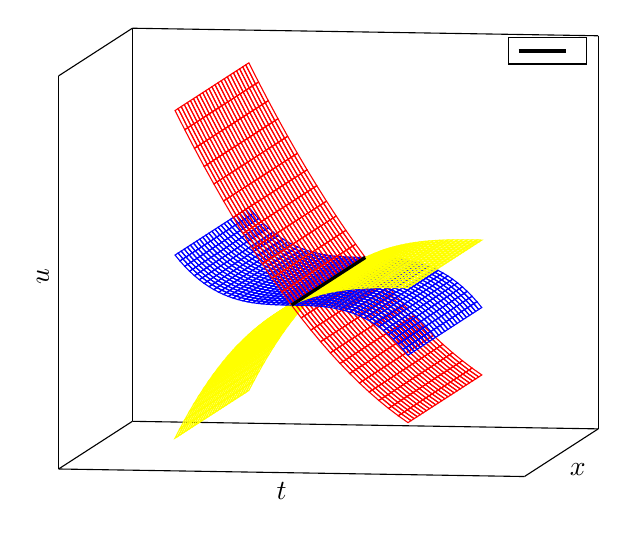
\begin{tikzpicture}
  \begin{axis}[view={99}{7},ticks=none,xlabel=$x$,ylabel=$t$,zlabel=$u$,ymin=-1.,ymax=1.]
    \addplot3[black,very thick,domain=-4:4,samples=60,samples y=0]({x},{0.},{5.});

    \addplot3[mesh,draw=Yellow,domain=-4:4,y domain=-0.5:0.] {2.*(y-0.5)^3+(2.*(0.5)^3)+5.};
    \addplot3[mesh,draw=Blue,domain=-4:4,y domain=-0.5:0.] {-5.*y^3+5.};
    \addplot3[mesh,draw=Red,domain=-4:4,y domain=-0.5:0.5] {2.*(y-1.)^2 -2. +5.};
    \addplot3[mesh,draw=Blue,domain=-4:4,y domain=-0.:0.5] {-5.*y^3+5.};
    \addplot3[mesh,draw=Yellow,domain=-4:4,y domain=-0.:0.5] {2.*(y-0.5)^3+(2.*(0.5)^3)+5.};
    \addplot3[black,very thick,domain=-4:4,samples=60,samples y=0]({x},{0.},{5.});
    \legend{$\Cscr$}
  \end{axis}
\end{tikzpicture}
%%% Local Variables:
%%% mode: latex
%%% TeX-master: "../../mainManuscript"
%%% End:
} \qquad 
%   \subcaptionbox{Projection in $(t,u)$ plane\label{subfig:fan_plan_proj}}{\begin{tikzpicture}
  \begin{axis}[ticks=none,xlabel=$t$,ylabel=$u$]
    \addplot[Red,very thick,domain=-0.5:0.5] {2.*(x-1.)^2 -2. +5.};
    \addplot[Red,thick,domain=-0.5:0.5] {-4.*x+5.};
    \addplot[Blue,very thick,domain=-0.5:0.5] {-5.*x^3+5.};
    \addplot[Blue,thick,domain=-0.5:0.5] {5.};
    \addplot[Duck,very thick,domain=-0.5:0.5] {2.*(x-0.5)^3+(2.*(0.5)^3)+5.};
    \addplot[Duck,thick,domain=-0.5:0.5] {1.5*x+5.};
    % \addplot3[black,very thick,domain=-5:5,samples=60,samples y=0]({x},{0.},{x^2+5.});
  \end{axis}
\end{tikzpicture}
%%% Local Variables:
%%% mode: latex
%%% TeX-master: "../../mainManuscript"
%%% End:
}
%   \caption{Examples of integral surfaces passing through the same initial curve $\Cscr$ defined such that $t=const$ and $u=const$ along $\Cscr$.}
%   \label{fig:plan_fan}
% \end{figure}
This defines \textit{characteristic line elements} tangent to all integral surfaces $u^{(i)}(x,t)$:
\begin{equation}
  \label{eq:monge_axis}
  \matrice{dx \\ dt \\ du} = \matrice{a \\ b \\c}
\end{equation}
\begin{figure}[h!]
  \centering
  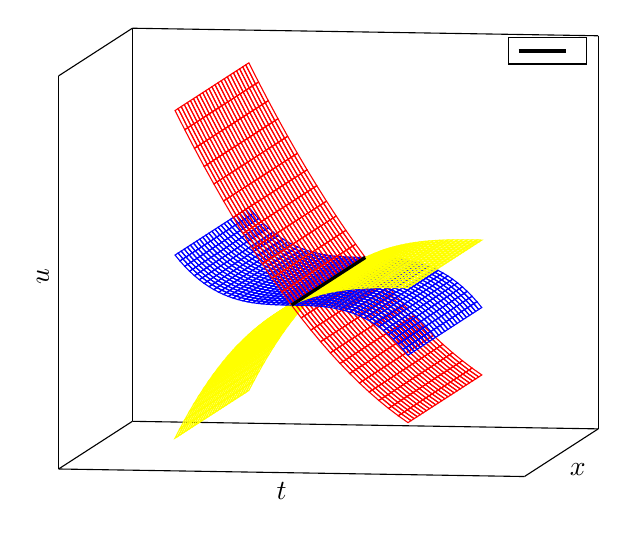
\begin{tikzpicture}
  \begin{axis}[view={99}{7},ticks=none,xlabel=$x$,ylabel=$t$,zlabel=$u$,ymin=-1.,ymax=1.]
    \addplot3[black,very thick,domain=-4:4,samples=60,samples y=0]({x},{0.},{5.});

    \addplot3[mesh,draw=Yellow,domain=-4:4,y domain=-0.5:0.] {2.*(y-0.5)^3+(2.*(0.5)^3)+5.};
    \addplot3[mesh,draw=Blue,domain=-4:4,y domain=-0.5:0.] {-5.*y^3+5.};
    \addplot3[mesh,draw=Red,domain=-4:4,y domain=-0.5:0.5] {2.*(y-1.)^2 -2. +5.};
    \addplot3[mesh,draw=Blue,domain=-4:4,y domain=-0.:0.5] {-5.*y^3+5.};
    \addplot3[mesh,draw=Yellow,domain=-4:4,y domain=-0.:0.5] {2.*(y-0.5)^3+(2.*(0.5)^3)+5.};
    \addplot3[black,very thick,domain=-4:4,samples=60,samples y=0]({x},{0.},{5.});
    \legend{$\Cscr$}
  \end{axis}
\end{tikzpicture}
%%% Local Variables:
%%% mode: latex
%%% TeX-master: "../../mainManuscript"
%%% End:

  \caption{Examples of integral surfaces passing through the same curve $\Cscr$ defined such that $t=const$ and $u=const$ along $\Cscr$.}
  \label{fig:plan_fan}
\end{figure}
Introduction of a parameter $\eta$ and integration of equation \eqref{eq:monge_axis} yields a one-parameter family of \textit{characteristic curves} of the PDE:
\begin{equation*}
  x=x(\eta) \quad ; \quad t=t(\eta) \quad ; \quad u=u(\eta)
\end{equation*}
Hence, a characteristic curve is tangent at every point to all the integral surfaces, and an infinity of integral surfaces cross one characteristic curve. As a consequence, if the initial curve is a characteristic curve, infinitely many integral surfaces contain it so that the Cauchy problem can not be solved.

However, the following statement holds \cite[Ch.1]{Courant}:
\begin{theorem}[Courant]
  \label{th:integral_surface_generated}
  Every surface $u(x,t)$ generated by a one-parameter family of characteristic curves is an integral surface. Conversely, every integral surface is generated by a one-parameter family of characteristic curves.
\end{theorem}
This theorem will be used in what follows to solve the Cauchy problem.

\subsection{The method of characteristic}
We now extend the concept of characteristic curves to first order quasi-linear systems of dimension $I$. In matrix form:
\begin{equation}
  \label{eq:1st_order_quasi-linear_syst}
  \Absf^t\(x,t,\vect{\Uc}\) \: \vect{\Uc}_t + \Absf^x\(x,t,\vect{\Uc}\)\: \vect{\Uc}_x + \vect{\Sc} = \vect{0}
\end{equation}
Similarly to quasi-linear PDEs, given values of $\Ucb$ are prescribed along a regular curve $\Cscr_0:\varphi(x,t)=const$ defining the initial curve $\Ucb(\varphi(x,t))$ of the $(x,t,\Ucb)$ space. The Cauchy problem consists in finding all the derivatives of $\Ucb(x,t)$ such that equation \eqref{eq:1st_order_quasi-linear_syst} is satisfied in the vicinity of $\Cscr$.
Noticing that along the initial curve $\Ucb_x = \Ucb' \varphi_x$ and $\Ucb_t = \Ucb' \varphi_t$, one gets:
\begin{equation*}
  \vect{\Uc}_x\varphi_t - \vect{\Uc}_t\varphi_x= \vect{0}
\end{equation*}
Hence, system \eqref{eq:1st_order_quasi-linear_syst} can be rewritten:
\begin{equation}
  \label{eq:normal_form}
  \( \Absf^x - \lambda \Absf^t \) \vect{\Uc}_x + \vect{\Sc} = \vect{0} 
\end{equation}
where:
\begin{equation}
  \label{eq:lambda_slope}
  \lambda=-\frac{\varphi_t}{\varphi_x}=\ddroit{x}{t}
\end{equation}
The Cauchy problem admits n unique solution $\vect{\Uc}_x$ along $\Cscr$ if the determinant of the system does not vanish, that is:
\begin{equation}
  \label{eq:characteristic_determinant}
  D=\abs{\Absf^x - \lambda \Absf^t} \ne 0
\end{equation}
where D is called the \textit{characteristic determinant} of system \eqref{eq:1st_order_quasi-linear_syst}. If D does not have real roots along $\Cscr_0$, the problem is said \textit{elliptic} and the Cauchy problem can be solved. Indeed, in that case the knowledge of $\Ucb$ along the initial curve allows the computation of derivatives and hence, the building of an integral strip defined by $\Ucb,\Ucb_x,\Ucb_t$. If equation \eqref{eq:1st_order_quasi-linear_syst} admits $I$ real roots on the other hand, system \eqref{eq:normal_form} can no longer be solved. Those eigenvalues come along with left and right eigenvectors respectively defined as:
\begin{equation}
  \label{eq:eigenvectors}
  \Lc^k_i  \Asf^x_{ij} = \lambda_k \Lc^k_i \Asf^t_{ij} \quad ; \quad \Asf^x_{ij}\Rc^k_j = \lambda_k \Asf^t_{ij}\Rc^k_j \qquad k=1,...,I
\end{equation}
\begin{remark}
  Note that eigenvectors can be stored as matrices $\Rbsf$ and $\Lbsf$ where $\Rsf_{ij}=\Rc^j_i$ and $\Lsf_{ij}=\Lc_j^i$.
\end{remark}

A first order system of $I$ partial differential equations is said \textit{hyperbolic} if it admits $I$ real eigenvalues associated to independent eigenvectors \cite{Courant}.
For those problems one can draw a set of one-parameter families of curves in the $(x,t)$ plane by integrating the relations $\lambda_k=dx/dt$ ($1 \leq k \leq I$).
\begin{example}
  \label{ex:charac1}
  Consider the first order system with variable coefficients
\begin{equation*}
 \matrice{x &0 \\0 &-x} \drond{}{t} \matrice{\Uc_1 \\ \Uc_2} + \drond{}{x}\matrice{\Uc_1 \\ \Uc_2} = \matrice{0 \\0}
\end{equation*}
which characteristic determinant \eqref{eq:characteristic_determinant} is:
\begin{equation*}
  (1-\lambda x)(1+\lambda x)=0
\end{equation*}
We thus have two solutions $\lambda_{1,2}=\pm 1/x$ leading, by integration of \eqref{eq:lambda_slope}, to two one-parameter families of characteristic curves:
\begin{equation*}
  t_1(x)=\frac{1}{2}x^2+c_1  \quad \text{and} \quad t_2(x)=-\frac{1}{2}x^2+c_2 
\end{equation*}
Those curves are drawn in figure \ref{fig:exampleCharac}\subref{subfig:curve_lines} for several values of integration constants $c_1$ and $c_2$.
\end{example}
\begin{example}
  \label{ex:charac2}
  Consider now the first order system with constant coefficients
\begin{equation*}
 \matrice{1 &0 \\0 &2} \drond{}{t} \matrice{\Uc_1 \\ \Uc_2} + \drond{}{x}\matrice{\Uc_1 \\ \Uc_2} = \matrice{0 \\0}
\end{equation*}
which eigenvalues, according to equation \eqref{eq:characteristic_determinant} satisfy
\begin{equation*}
  (1 - \lambda )(1- 2\lambda)=0
\end{equation*}
Two real roots exist $\lambda_1=1 \: ; \: \lambda_2=1/2$, leading by integration of \eqref{eq:lambda_slope} to two one-parameter families of straight lines:
\begin{equation*}
  t_1(x)=x+c_1  \quad \text{and} \quad t_2(x)=2x+c_2 
\end{equation*}
Unlike example \ref{ex:charac1}, coefficient matrices do not depend on independent variables, thus yielding to characteristic straight lines in the $(x,t)$ plane (see \ref{fig:exampleCharac}\subref{subfig:straight_lines}).
\end{example}
\begin{figure}[h]
  \centering
  \subcaptionbox{Example \ref{ex:charac1}: $\lambda_{1,2}=\pm 1/x$\label{subfig:curve_lines}}{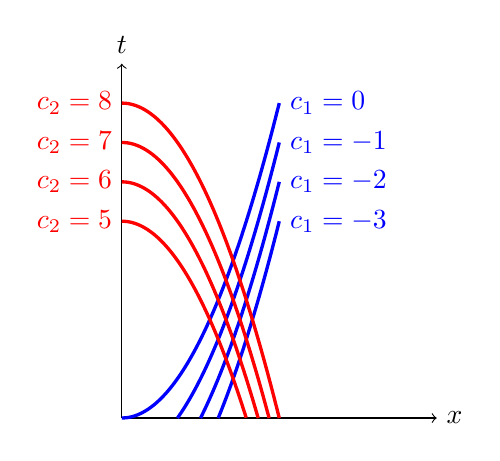
\begin{tikzpicture}
  \draw[->] (0,0) -- (4.,0) node[right] {$x$};
  \draw[->] (0,0) -- (0,4.5) node[above] {$t$};
  \draw[scale=0.5,domain=0:4,smooth,variable=\x,Blue,very thick] plot ({\x},{0.5*\x*\x}) node [right] {$c_1=0 $};
  \draw[scale=0.5,domain=1.4142:4,smooth,variable=\x,Blue,very thick] plot ({\x},{0.5*\x*\x-1}) node [right] {$c_1=-1$};
  \draw[scale=0.5,domain=2:4,smooth,variable=\x,Blue,very thick] plot ({\x},{0.5*\x*\x-2}) node [right] {$c_1=-2$};
  \draw[scale=0.5,domain=2.44948:4,smooth,variable=\x,Blue,very thick] plot ({\x},{0.5*\x*\x-3}) node [right] {$c_1=-3$};
  \draw[scale=0.5,domain=0:3.16,smooth,variable=\x,Red,very thick] plot ({\x},{-0.5*\x*\x+5});
  \node[left,Red] at (0,2.5) {$c_2=5$};
  \draw[scale=0.5,domain=0:3.4641,smooth,variable=\x,Red,very thick] plot ({\x},{-0.5*\x*\x+6});
  \node[left,Red] at (0,3) {$c_2=6$};
  \draw[scale=0.5,domain=0:3.7416,smooth,variable=\x,Red,very thick] plot ({\x},{-0.5*\x*\x+7});
  \node[left,Red] at (0,3.5) {$c_2=7$};
  \draw[scale=0.5,domain=0:4,smooth,variable=\x,Red,very thick] plot ({\x},{-0.5*\x*\x+8});
  \node[left,Red] at (0,4) {$c_2=8$};
\end{tikzpicture}
%%% Local Variables:
%%% mode: latex
%%% TeX-master: "../../mainManuscript"
%%% End:
}
  \subcaptionbox{Example \ref{ex:charac2}: $\lambda_{1}=1 \:\text{and} \: \lambda_2=1/2$\label{subfig:straight_lines}}{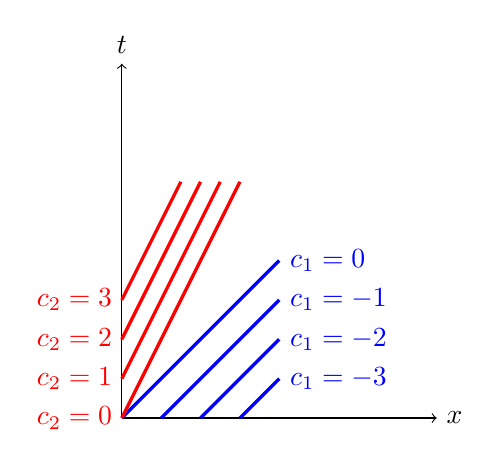
\begin{tikzpicture}
  \draw[->] (0,0) -- (4.,0) node[right] {$x$};
  \draw[->] (0,0) -- (0,4.5) node[above] {$t$};
  \draw[scale=0.5,domain=0:4,smooth,variable=\x,Blue,very thick] plot ({\x},{\x}) node [right] {$c_1=0$};
  \draw[scale=0.5,domain=1.:4,smooth,variable=\x,Blue,very thick] plot ({\x},{\x-1}) node [right] {$c_1=-1$};
  \draw[scale=0.5,domain=2:4,smooth,variable=\x,Blue,very thick] plot ({\x},{\x-2}) node [right] {$c_1=-2$};
  \draw[scale=0.5,domain=3:4,smooth,variable=\x,Blue,very thick] plot ({\x},{\x-3}) node [right] {$c_1=-3$};
  \draw[scale=0.5,domain=0:3,smooth,variable=\x,Red,very thick] plot ({\x},{2*\x});
  \node[left,Red] at (0,0) {$c_2=0$};
  \draw[scale=0.5,domain=-0.:2.5,smooth,variable=\x,Red,very thick] plot ({\x},{2*\x+1});
  \node[left,Red] at (0,0.5) {$c_2=1$};
  \draw[scale=0.5,domain=-0:2,smooth,variable=\x,Red,very thick] plot ({\x},{2*\x+2});
  \node[left,Red] at (0,1) {$c_2=2$};
  \draw[scale=0.5,domain=-0:1.5,smooth,variable=\x,Red,very thick] plot ({\x},{2*\x+3});
  \node[left,Red] at (0,1.5) {$c_2=3$};
\end{tikzpicture}
%%% Local Variables:
%%% mode: latex
%%% TeX-master: "../../mainManuscript"
%%% End:
}
  \caption{Family of base characteristic curves corresponding to the eigenvalues of the first order systems given in examples \ref{ex:charac1} and \ref{ex:charac2}.}
  \label{fig:exampleCharac}
\end{figure}

As theorem \ref{th:integral_surface_generated} states, an integral surface is generated by a one-parameter family of characteristic curves. Therefore the knowledge of those curves can be used to build the solution of the Cauchy problem. Indeed, the projection of the quasi-linear system \eqref{eq:1st_order_quasi-linear_syst} onto the \textit{left eigenbasis} or \textit{left characteristic basis} leads to:
\begin{equation*}
  \vect{\Lc}^k \( \Absf^t \vect{\Uc}_t + \Absf^x\vect{\Uc}_x \) + \vect{\Lc}^k \vect{\Sc}= \vect{0}
\end{equation*}
%Introduction of the definition of left eigenvectors \eqref{eq:eigenvectors} then yields:
where $\Lcb^k$ satisfies \eqref{eq:eigenvectors}, and hence:
\begin{equation*}
  \vect{\Lc}^k  \Absf^t \( \vect{\Uc}_t +\lambda_k \vect{\Uc}_x   \) + \vect{\Lc}^k \vect{\Sc}=\vect{0}
\end{equation*}
In this equation, the \textit{directional derivative} of $\vect{\Uc}$ along the $k$th characteristic curve arises, namely:
\begin{equation*}
 \ddroit{\Ucb}{t}\lvert_{t\in\varphi^k} = \Ucb_t + \lambda_k \Ucb_x   
\end{equation*}
Thus, along a characteristic curve a system of partial differential equations reduces to a system of \textit{Ordinary Differential Equations} (ODEs) composed of the following \textit{characteristic equations}:
\begin{equation}
  \label{eq:PDEs_ODEs}
  \vect{\Lc}^k  \Absf^t \(\ddroit{\Ucb}{t} + \Scb \)=\vect{0}
\end{equation}
Integration of equations \eqref{eq:PDEs_ODEs} yields a set of \textit{integral curves} from which the Cauchy problem can be solved.
%It then comes out that the Cauchy problem can be solved as the system \eqref{eq:PDEs_ODEs}.
Indeed, the solution at a point of the $(x,t)$ plane can be determined by tracing backward the characteristic curves to the initial curve and integrating ODEs \eqref{eq:PDEs_ODEs} along those paths according to the \textit{method of characteristics}. Note that if the right-hand side of equation \eqref{eq:1st_order_quasi-linear_syst} is zero, then $\Ucb$ is constant along characteristic curves. 

To illustrate the method, let us consider again the quasi-linear system of example \ref{ex:charac1} for which the Cauchy problem is built by prescribing initial conditions along the $x$-axis. Note that "initial conditions" have now a physical meaning since they are defined at $t=0$, the Cauchy problem is then an \textit{Initial Value Problem (IVP)}. Through a point $(x^*,t^*)$ pass two characteristic curves, each belonging to a different one-parameter family. The solution at this point can be determined by integrating the ODE corresponding to the first (\textit{resp. second}) eigenvalue of the system between $(x^1,0)$ (\textit{resp. $(x^2,0)$}) and $(x^*,t^*)$. The singularity of hyperbolic problems can hence be circumvented by using the characteristic structure in order to determine n unique solution. 
\begin{figure}[h]
  \centering
  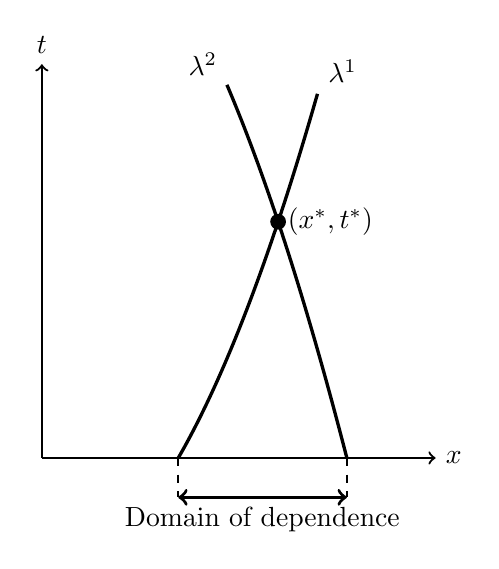
\begin{tikzpicture}
  \draw[thick,->](0,0)--(5,0) node [right] {$x$};
  \draw[thick,->](0,0)--(0,5) node [above] {$t$};
  % t1 = 0.5*x**2 + c1
  % t2 = -0.5*x**2 + c2
  % -> c1 = -1.5 ; c2 = 7.5
  % \draw[domain=1.7320508:3.5,smooth,variable=\x,Purple,very thick] plot ({\x},{0.5*\x*\x-1.5}) node [above right] {$t=\frac{x^2-3}{2}$};
  % \draw[domain=2.35:3.872983,smooth,variable=\x,Green,very thick] plot ({\x},{-0.5*\x*\x+7.5});
  \draw[domain=1.7320508:3.5,smooth,variable=\x,very thick] plot ({\x},{0.5*\x*\x-1.5}) node [above right] {$\lambda^1$};
  \draw[domain=2.35:3.872983,smooth,variable=\x,very thick] plot ({\x},{-0.5*\x*\x+7.5});
  % \node[left,Green] at (2.35,5) {$t=-\frac{x^2-15}{2}$};
  \node[left] at (2.35,5) {$\lambda^2$};
  \draw[<->,very thick] (1.7320508,-0.5) -- (3.872983,-0.5) ;
  \draw[dashed,thick] (1.7320508,0) -- (1.7320508,-0.5);
  \draw[dashed,thick] (3.872983,-0.) -- (3.872983,-0.5);
  \node[below] at (2.80,-0.5) {\text{Domain of dependence}};
  \fill[black] (3,3) circle (0.1) node [right] {$(x^*,t^*)$};
\end{tikzpicture}
%%% Local Variables:
%%% mode: latex
%%% TeX-master: "../../mainManuscript"
%%% End:

  \caption{Domain of dependence of the solution at point $(x^*,t^*)$ for the system of example \ref{ex:charac1}.}
  \label{fig:charac_method2x2}
\end{figure}
We see that only a segment of the initial curve has an influence on the solution at a given point. Namely, the intersections of the initial curve and characteristic curves with the highest and the lowest slopes define the \textit{domain of dependence} of the solution at this point (see figure \ref{fig:charac_method2x2}). This property of hyperbolic problems implies the existence of waves that propagates information at finite speeds corresponding to the eigenvalues of a quasi-linear form. The theory presented so far will be applied in what follows to solid mechanics.



%%% Local Variables:
%%% mode: latex
%%% TeX-master: "../mainManuscript"
%%% End:


\section{Governing equations of solid mechanics}
\label{sec:solidMech_equations}
In this section, the mathematical laws allowing the description of the deformation of a solid body will be derived. First, the kinematic laws governing the motion of each material point belonging to a solid will be considered. The variations of lengths and shapes of a continuum, described by the \textit{strain} mesure will then be associated to internal forces through thermodynamic framework. Finally, the theory of first order quasi-linear partial differential system will be applied to solid dynamics in order to deliver analytical solutions for specific problems. The literature on the subject being very rich (see for instance \cite[Chapters~1-3]{Foundation_of_elasticity}, \cite{Truesdell}, \cite[Chapter~7]{Simo}, \cite[Chapters~3 \& 5]{Belytschko}), the governing equations of mechanics will be developed non-exhaustively.

\subsection{Kinematic laws -- Strain mesures}
We consider a three-dimensional solid domain with volume denoted by $\Omega \subset \Rbb^3$ bounded by the surface $\partial \Omega$. This body undergoes external sollicitations that can either be localized on a part of the external surface of the body (\textit{i.e. surface forces}) or act in the whole solid domain (\textit{i.e. volume forces}). Due to the presence of such sollicitations, the volume may change during a deformation within the time interval $\tau = \[0,T\]$ and will hence be written as a function of time $\Omega(t)$ ($t\in \tau$). The state of the solid at time $t=0$, corresponding to a non-deformed state with volume $\Omega(t=0)=\Omega_0$, is referred to as the \textit{initial configuration}. Some problems require the use of a \textit{reference configuration} that can be deformed and to which equations are referred. In what follows, the reference and initial conditions are identical. At a given time $t>0$, the volume $\Omega(t)=\Omega_t$ corresponds to the \textit{current configuration}. These configurations are depicted in figure \ref{fig:deformationFunction}.
\begin{figure}[h]
  \centering
  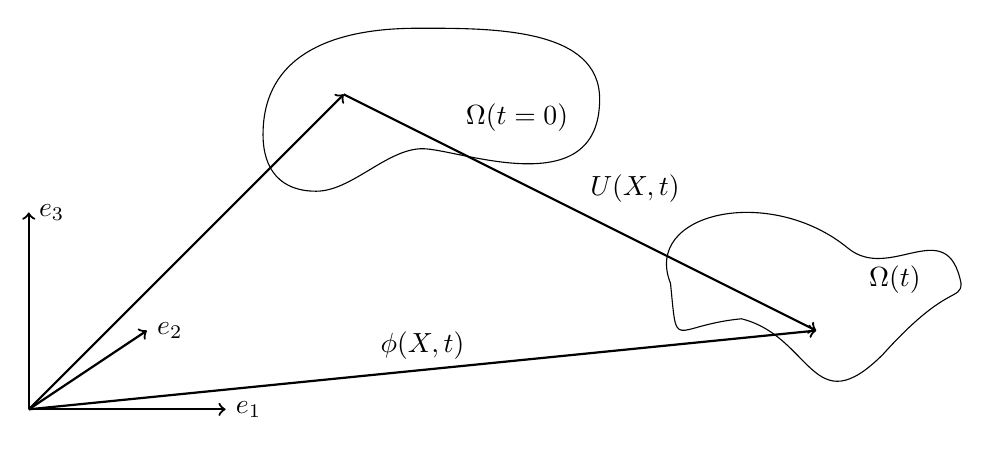
\begin{tikzpicture}
  %\draw[step=1.0,black,thin] (-3.,-1.) grid (3,4.);
  %\draw (-3,-1) -- (3,-1) -- (3,4) -- (-3,4) -- (-3,-1);
  \draw[thick,->] (-5,-2.5) -- (-2.5,-2.5) node [right] {$\vect{e}_1$};
  \draw[thick,->] (-5,-2.5) -- (-5,0.) node [right] {$\vect{e}_3$};
  \draw[thick,->] (-5,-2.5) -- (-3.5,-1.5) node [right] {$\vect{e}_2$};
  \begin{scope}[scale=0.45]
    \draw (-3,0.6) .. controls +(1,0) and +(-1,0) .. (0,1.8)  
    .. controls +(1,0) and +(0,-3) .. (5,3.2) 
    .. controls +(0,2) and +(2,0)  .. (0,5.2) 
    .. controls +(-1,0) and +(0,3) .. (-4.5,2.2) 
    .. controls +(0,-1) and +(-1,0).. (-3,0.6) ;
  \end{scope}
  \node at (1.2,1.2) {$\Omega(t=0)$};
  %% Deformed body +2.
  \begin{scope}[scale=0.9]
    \draw (0.+0.5+4.,0-1.5) ..controls (1.+0.5+4.,-0.25-1.5) and (1.+0.5+4.,-1.5-1.5) .. (2.+0.5+4.,-0.5-1.5) ..controls (2.9+0.5+4.,0.5-1.5) and (3.1+0.5+4.,0.25-1.5) .. (3.1+0.5+4.,0.5-1.5) ..controls (2.9+0.5+4.,1.5-1.5) and (2.1+0.5+4.,.5-1.5) .. (1.5+0.5+4.,1.-1.5) ..controls (0.4+0.5+4.,1.9-1.5) and (-1.4+0.5+4.,1.5-1.5) .. (-1.+0.5+4.,0.5-1.5)..controls (-0.4+0.+4.,-0.-2.) and (-1+0.5+4.,0.4-2.) .. (0+0.5+4.,0-1.5);
  \end{scope}
  \node at (6.,-0.85) {$\Omega(t)$};
  \draw[->,thick] (-5,-2.5) -- (-1.,1.5) node [midway,left] {$\X$};
  \draw[->,thick] (-5,-2.5) -- (5.,-1.5) node [midway,above] {$\vect{\phi}(\vect{X},t)$};
  \draw[->,thick] (-1.,1.5) -- (5.,-1.5) node [midway,above right] {$\vect{U}(\vect{X},t)$};
\end{tikzpicture}

%%% Local Variables:
%%% mode: latex
%%% TeX-master: "../../mainManuscript"
%%% End:
  \caption{Deformation of a solid body between a reference state $\Omega_0$ to a subsequent state $\Omega_t$.}
  \label{fig:deformationFunction}
\end{figure}

In the reference configuration, every material particle is located by their position vectors: $\vect{X}=X_\alpha \vect{e}_\alpha$, where $X_\alpha$ denotes the \textit{Lagrangian coordinates} and $\vect{e}_\alpha$ the basis vectors. At a subsequent time $t$, the particle initially located at $\vect{X}$ may have moved and its current location is given by the smooth mapping $\vect{\phi}(\vect{X},t)=\phi_i(\vect{X},t)\vect{e}_i$. Thus, the mapping $\vect{\phi}$ provides the paths of every particle of the solid during the deformation. In the lagrangian coordinates system, every particles are tracked during the deformation while the \textit{Eulerian coordinates}, denoted by $\vect{x}=x_i\vect{e}_i$, correspond to a \textit{spatial description}.
Note that in the above definitions Greek indices are used for quantities evaluated in the reference configuration whereas Latin ones refer to quantities defined in the current configuration. 

The \textit{displacement} and \textit{velocity} vectors of a particle between the reference and the current configuration are respectively:
\begin{subequations}
  \begin{alignat}{2}
    &\vect{u}(\vect{X},t)=\vect{\phi}(\vect{X},t) - \vect{X} \qquad \forall\:\: \vect{X},t \in \Omega_0\times \tau  \label{eq:displacement}\\
    &\vect{v}(\vect{X},t)=\drond{\vect{\phi}}{t}(\vect{X},t) = \vect{\dot{\phi}}(\vect{X},t) \qquad  \forall\: \: \vect{X},t \in \Omega_0\times \tau  \label{eq:velocity}
  \end{alignat}
\end{subequations}
where the superposed dot denotes the material time derivative. Then, the second-order two-point \textit{deformation gradient} tensor is defined as:
\begin{equation}
  \label{eq:F_phi}
    \tens{F}=\nablat_0 \vect{\phi} (\vect{X},t)
\end{equation}
where $\nablat_0 (\bullet)$ refers to the gradient operator on the reference configuration. This tensor can also be written by using equation \eqref{eq:displacement}:
\begin{equation}
  \tens{F}= \nablat_0 \vect{u}(\vect{X},t) + \tens{I} \label{eq:F_displacement}
\end{equation}
with $\tens{I}$, the second-order identity tensor. The deformation gradient tensor characterizes the variations of lengths, areas and volumes. Indeed, the infinitesimal vector, oriented surface and volume elements respectively denoted by $\vect{dX},\vect{dS}$ and $dV$ and defined in the reference configuration transorm respectively to:
\begin{equation}
  \label{eq:transport_equations}
  \begin{aligned}
    & dx_i=F_{i\alpha}dX_\alpha \\
    & ds_i=J F_{\alpha i}^{-1}dS_{\alpha} \\
    & dv=JdV 
  \end{aligned}
\end{equation}
in the current configuration. The transport equations \eqref{eq:transport_equations} involve the determinant of the deformation gradient $J=\det(\tens{F})>0$, also called the \textit{Jacobian of the deformation}. The deformation gradient is a strain mesure since it accounts for changes in lengths and angles (\textit{i.e. the change of shape of a body}). Other strain mesures can be used as the \textit{right Cauchy-Green} or the \textit{Green-Lagrange} tensors, respectively defined as:
\begin{equation*}
  \begin{aligned}
    & \tens{C}=\tens{F}^T\tens{F} \\
    & \tens{E}=\frac{1}{2}(\tens{C}-\tens{I})
  \end{aligned}
\end{equation*}
where $\tens{I}$ is the second-order identity tensor. The Green-Lagrange tensor can also be written by means of equation \eqref{eq:F_displacement}:
\begin{equation*}
  \tens{E}=\frac{1}{2}(\nablat_0 \vect{u} + \nablat_0 \vect{u}^T + \nablat_0 \vect{u}\nablat_0 \vect{u}^T)
\end{equation*}
In particular, when the deformation involves displacement vectors such that $\norm{\nablat_0 \vect{u}} \ll 1$, the last (second-order) term of the previous definition can be neglected leading to:
\begin{equation*}
  \tens{E} \approx \frac{1}{2}(\nablat_0 \vect{u} + \nablat_0 \vect{u}^T) = \tens{\eps}
\end{equation*}
with $\tens{\eps}$ the \textit{linearized strain tensor}, the symmetric part of the displacement gradient. Such deformations fall in the \textit{linearized geometrical framework} and are characterized by small strain but possibly large displacements. Furthermore, when the deformation leads to a displacement vector $\norm{\vect{u}} \ll 1$ reference and current configurations are considered as indentical. These situations correspond to the \textit{small strain} framework for which the reference and current configurations are considered as identical.

\subsection{Balance equations}
In this section a solid domain $\Omega(t)$ undergoing a deformation is still considered within the time interval $\tau = \[0,T\]$. We start the development of balance laws that hold in the continuum during the deformation by the conservation of mass of a conntinuum, which in integral form reads:
\begin{equation*}
  \int_\Omega \rho d\Omega = \int_{\Omega_0} \rho_0 d\Omega \qquad \forall \: t \in  \tau
\end{equation*}
which, with the third transport formula reads:
\begin{equation}
  \label{eq:mass_conservation_law}
  \int_{\Omega_0} \(J\rho - \rho_0\) d\Omega = 0
\end{equation}
Leading to the first balance equation, namely the local conservation of mass:
\begin{equation}
  \label{eq:mass_balance}
  \rho = \frac{\rho_0}{J} \qquad \forall \: \vect{X},t \: \in \Omega_0\times \tau
\end{equation}

We now move on to the equilibrium between acceleration effects, namely \textit{intertia}, and external forces undergone by a solid $\Omega$. This conservation law corresponds to \textit{Newton's second law}:
\begin{equation*}
  \int_\Omega \rho \vect{\dot{v}} d\Omega = \int_{\partial \Omega} \vect{t} dS + \int_{\Omega} \rho\vect{b}d\Omega \qquad \forall \: t \in  \tau
\end{equation*}
where $\vect{t}$ denotes surface forces and $vect{b}$ volume forces in the current configuration. We then introduce the symetric second-order \textit{Cauchy stress tensor} $\tens{\sigma}$ by using Cauchy's theorem $\vect{t}=\tens{\sigma}\cdot \vect{n}$ where $\vect{n}$ is the outwerd normal vector to the surface element $dS$. 

For further developments, the divergence theorem is required:
\begin{equation}
  \label{eq:Ostrogradski_th}
  \int_{\partial \Omega} (\bullet)\cdot \vect{dS}=\int_\Omega \nablav \cdot (\bullet) \: d\Omega
\end{equation}
where $\nablav \cdot (\bullet)$ denotes the divergence operator on the current configuration. Introduction of the previous formula in the second law of Newton leads to:
\begin{equation}
  \label{eq:Linear_momentum_conservation_eulerian}
  \int_{\Omega} \( \rho \vect{\dot{v}} - \nablav \cdot \tens{\sigma} -  \rho\vect{b} \) d\Omega = \vect{0} \qquad \forall \:t \in  \tau
\end{equation}
Conservation law \eqref{eq:Linear_momentum_conservation_eulerian} can be mapped to the reference configuration by using the transport formula of volume elements and the mass balance equation \eqref{eq:mass_balance}, thus yielding:
\begin{equation}
  \label{eq:Linear_momentum_conservation}
  \int_{\Omega_0} \( \rho_0 \vect{\dot{v}} - J \nablav \cdot \tens{\sigma} -  \rho_0\vect{b} \) d\Omega = \vect{0} \qquad \forall \: t \in\tau
\end{equation}
In equation \eqref{eq:Linear_momentum_conservation}, the divergence operator on the current configuration can be transported to the reference one by means of the \textit{Piola transform}:
\begin{definition}
  The Piola--Kirchhoff tranform $\tens{T}^P$ of a second-order tensor $\tens{T}$ is defined as:
  \begin{equation*}
    \tens{T}^P=J\tens{T}\cdot\tens{F}^{-1}
  \end{equation*}
  and satisfies:
  \begin{equation*}
    \nablav_0\cdot \tens{T}^P = J \nablav \cdot \tens{T}
  \end{equation*}
  where $\nablav_0\cdot (\bullet)$ is the divergence operator on the reference configuration.
\end{definition}
Another stress mesure that corresponds to the Piola transform of Cauchy stress tensor is thus introduced, the \textit{first Piola-Kirchhoff stress tensor} $\tens{\Pi}=J\tens{\sigma}\cdot\tens{F}^{-1}$. Hence, the vanishing of the integrand in equation \eqref{eq:Linear_momentum_conservation} yields the balance equation of the \textit{lagrangian linear momentum}:
\begin{equation}
  \label{eq:Lagrangian_linear_momentum}
  \rho_0 \vect{\dot{v}} - \nablav_0 \cdot \tens{\Pi} = \rho_0 \vect{b} \qquad \forall \: \: \vect{X},t \in \Omega_0 \times \tau 
\end{equation}
When considering deformations within the small strain framework the balance equation of linear momentum can be deduced from equation \eqref{eq:Linear_momentum_conservation_eulerian}, leading to:
\begin{equation}
  \label{eq:HPP_linear_momentum}
  \rho \vect{\dot{v}} - \nablav \cdot \tens{\sigma} = \rho \vect{b}  \qquad \forall \: \: \vect{x},t \in \Omega \times \tau 
\end{equation}

We complete the set of balance laws by considering the conservation of the energy of a system, also known as the \textit{first law of thermodynamics}. This law relates a balance between the rates of change of \textit{kinetic} and \textit{internal} energies, the power of external forces and the amount of heat entering the system as \textit{volume} or \textit{surface heat sources}.
\begin{equation*}
  \ddroit{}{t}\int_{\Omega} \(\frac{1}{2}\rho \vect{v}\cdot\vect{v} + \rho e\) d\Omega = \int_{\partial \Omega} \(\tens{\sigma}\cdot\vect{n}\)\cdot\vect{v} \: dS + \int_{\Omega} \rho\vect{b}\cdot\vect{v} \: d\Omega + \int_{\Omega} \rho r \:d\Omega - \int_{\partial \Omega} \vect{q}\cdot\vect{n} \: dS \qquad \forall \: t \in  \tau 
\end{equation*}
where $\vect{q}$ is the outward heat flux vector and $r$ is a volume heat source. By using the divergence theorem \eqref{eq:Ostrogradski_th}, the previous equation reads:
\begin{equation*}
\ddroit{}{t}\int_{\Omega} \(\frac{1}{2}\rho \vect{v}\cdot\vect{v} + \rho e\) d\Omega = \int_{\Omega} \(\nablav\cdot(\tens{\sigma}\cdot\vect{v}) +  \rho\vect{b}\cdot\vect{v} \) d\Omega + \int_{\Omega} \rho r \: d\Omega  - \int_{\partial \Omega} \vect{q}\cdot\vect{n} \: dS \qquad \forall \: t \in  \tau 
\end{equation*}
The transport of this relation on the reference configuration based on \eqref{eq:transport_equations} allows to introduce the time derivative of the left-hand side in the integral
\begin{equation*}
\int_{\Omega_0} \(\rho_0 \vect{\dot{v}} + \rho_0 \dot{e}\) d\Omega = \int_{\Omega_0} \(J\nablav\cdot(\tens{\sigma}\cdot\vect{v}) +  \rho_0\vect{b}\cdot\vect{v} \) d\Omega + \int_{\Omega_0} \rho_0 r \:d\Omega- \int_{\partial \Omega_0} J\vect{q}\cdot \tens{F}^{-1}\cdot\vect{n} \: dS \qquad \forall \: t \in  \tau 
\end{equation*}
Then, substitution of the linear momentum according to equation \eqref{eq:Lagrangian_linear_momentum} yields, after some algebra, the conservation law of internal energy:
\begin{equation}
  \label{eq:conservation_law_energy}
  \int_{\Omega_0} \rho_0 \dot{e} d\Omega = \int_{\Omega_0} \tens{\Pi}:\nablat_0\vect{v}\: d\Omega + \int_{\Omega_0} \(\rho_0r  - \nablav_0 \cdot \vect{Q}\) d\Omega \qquad \forall \: t \in  \tau 
\end{equation}
where $\vect{Q}=J\vect{q}\cdot \tens{F}^{-1}$ is the lagrangian heat flux vector. We thus deduce the balance equation of internal energy on the reference configuration:
\begin{equation}
  \label{eq:energy_balance}
  \rho_0 \dot{e} -  \tens{\Pi}:\nablat_0\vect{v}  + \nablav_0 \cdot \vect{Q}  = r \qquad \forall \: \: \vect{X},t \in \Omega_0 \times \tau 
\end{equation}
where $\nablat_0\vect{v} = \tens{\dot{F}}$. Finally, the small strain version of equation \eqref{eq:energy_balance} is: 
\begin{equation}
  \label{eq:energy_balance}
  \rho \dot{e} -  \tens{\sigma}:\nablat^{s} \vect{v}  + \nablav \cdot \vect{q}  = r \qquad \forall \: \: \vect{x},t \in \Omega \times \tau 
\end{equation}
in which $\nablat^{s} (\bullet)$ denotes the symetric part of the gradient, in particular: $\nablat^s \vect{v} = \tens{\dot{\eps}}$. Stress mesures are conjugate to strain mesures through the power. In what follows, stress and strain may respectively be refered to as \textit{thermodynamic forces} and \textit{internal variables} according to the thermodynamics framework. The former obey a \textit{state equation} while the latter describe the evolution of the thermodynamic system. 
\subsection{Constitutive equations}
The closure of a problem is given by the constitutive equations (\textit{i.e state laws}) for the stress. Once and for all, we consider here constitutive models within the \textit{Generalized Standard Materials} (GSM) framework \cite{GSM}.

\subsubsection*{The general (hyper)elasticity formulation}
First, the \textit{Clausius-Duhem} inequality resulting from combination of first and second laws of thermodynamics, reads: 
\begin{equation}
  \label{eq:Clausius-Duhem}
  \underbrace{\phantom{\frac{1}{\theta}} \tens{\Pi}:\tens{\dot{F}} + \rho_0 \(\theta \dot{\eta} -\dot{e}\)}_{\Dc^{int}} \:-\:  \underbrace{\frac{1}{\theta} \vect{q} \cdot \nablav_0 \theta}_{-\Dc^{th}} \geq 0  \qquad \forall \: \: \vect{X},t \in \Omega_0 \times \tau 
\end{equation}
where $\Dc^{int}$ and $\Dc^{th}$ are respectively the specific mechanical and thermal dissipations, and $\eta, \theta$ denote \textit{entropy} and \textit{temperature}. Equation \eqref{eq:Clausius-Duhem} results in vanishing dissipations for \textit{reversible} processes and in a strict inequality for \textit{irreversible} ones. Furthermore, a widely used assumption consists in considering that the mechanical and thermal dissipations simultaneously satisfy non-negativeness. Note that the \textit{Fourier's law} of conduction is based on the non-negativeness of the thermal dissipation and leads to the following definition of the heat flux vector in order to ensure the positivity of the thermal dissipation:
\begin{equation*}
  \label{eq:Fourier_law}
  \vect{q}=-\tens{k}\cdot\nablav_0 \theta
\end{equation*}


We assume the existence of a \textit{Helmholtz free energy density potential} $\psi\(\tens{F},\theta,V_p\)$ where the $V_p$ $(1\leq p \leq N)$ are additional state variables describing irreversible processes. The free energy is supposed concave with respect to temperature and convex with respect to other variables. The mechanical dissipation then can be rewritten as:
\begin{equation*}
  \Dc^{int} = \tens{\Pi}:\tens{\dot{F}} - \rho_0 \(\dot{\psi} +\eta \dot{\theta}\) 
\end{equation*}
The time derivative of Helmholtz free energy:
\begin{equation*}
  \dot{\psi} = \drond{\psi}{\tens{F}}:\tens{\dot{F}} + \drond{\psi}{\theta}\dot{\theta} + \drond{\psi}{V_p}\dot{V_p}
\end{equation*}
can be introduced within the mechanical dissipation so that one gets:
\begin{equation}
  \label{eq:Dint_psi_factor}
  \Dc^{int} = \(\tens{\Pi}- \rho_0 \drond{\psi}{\tens{F}} \):\tens{\dot{F}} - \rho_0 \(\drond{\psi}{\theta} +\eta\) \dot{\theta}  - \rho_0\drond{\psi}{V_p}\dot{V_p} 
\end{equation}


Since the mechanical dissipation must be non-negative regardless of the nature of the deformation, it must in particular vanish for a reversible isothermal process (\textit{i.e. $\theta=const$}) for which every additional internal variables are constant. With these considerations, we are left with the relation:
\begin{equation*}
  \( \tens{\Pi} - \rho_0\drond{\psi}{\tens{F}} \): \tens{\dot{F}} = 0
\end{equation*}
holding regardless of the deformation, and hence:
\begin{equation}
  \label{eq:PK1_definition}
  \rho_0\drond{\psi}{\tens{F}} = \tens{\Pi}
\end{equation}
A material is said \textit{hyperelastic} if the above stress state law is satisfied \cite[p.8]{Foundation_of_elasticity}. Equivalently we have for linear elasticity:
\begin{equation}
  \label{eq:Cauchy_definition}
  \rho \drond{\psi}{\tens{\eps}} = \tens{\sigma}
\end{equation}

Similar considerations lead to the state laws for entropy and for additional thermodynamic forces :
\begin{equation*}
  %\label{eq:entropy_definition}
  \drond{\psi}{\theta} = - \eta \quad ; \quad \rho_0\drond{\psi}{V_p}=A_p
\end{equation*}

In what follows, we shall consider hyperelastic or linear elastic deformations that do not involve irreversible processes (\textit{e.g. damage or thermal softening}). Hence, additional internal variables and associated thermodynamic forces are not activated in such situations. However, the cases of \textit{elastoplasticity} and \textit{elasto-viscoplasticity}, involving such variables and forces, will be considered in the linearized geometrical framework.

\subsubsection*{History-dependent models in small strain}
% \subsubsection{Homogeneous systems}
% \subsubsection{Non-homogeneous systems}
\subsection{The general formulation}
We introduced above for the general case the balance equations of linear momentum \eqref{eq:Lagrangian_linear_momentum} and internal energy \eqref{eq:energy_balance}. Moreover, state equations of thermodynamic forces have been derived (equation \eqref{eq:PK1_definition} for stress and equation \eqref{eq:entropy_definition} for entropy). Those thermodynamic forces are dual quantities of internal variables (respectively strain and temperature) which variations govern the evolution of the system. Whereas the evolution of the deformation gradient is given by lagrangian kinematic law \eqref{eq:F_phi} written in rate form, the evolution of the temperature is governed by the well-known \textit{heat equation}:
\begin{equation}
  \label{eq:heat_equation}
  \rho_0 C \dot{\theta} = r - \nablav \cdot \vect{q} - \rho_0 \drond{\psi}{V_p}\dot{V_p} + \theta \(\drond{\tens{\Pi}}{\theta}:\tens{\dot{F}} - \drond{A_p}{\theta}\dot{V_p} \)
\end{equation}
For isothermal processes, the heat equation \eqref{eq:heat_equation} yields:
\begin{equation*}
  r - \nablav \cdot \vect{q} = \rho_0 \drond{\psi}{V_p}\dot{V_p} 
\end{equation*}
Also, such a deformation leads to the rate of change of internal energy:
\begin{align*}
  \rho_0 \dot{e} &= \rho_0 \( \dot{\psi} + \theta\dot{\eta}+\eta\dot{\theta}\) \\
                 &= \underbrace{\rho_0\drond{\psi}{\tens{F}}}_{=\tens{\Pi}}:\tens{\dot{F}} + \rho_0\underbrace{\drond{\psi}{\theta}}_{=-\eta}\dot{\theta} + \underbrace{\rho_0\drond{\psi}{V_p}}_{r - \nablav \cdot \vect{q}}\dot{V_p} + \rho_0\theta\dot{\eta}+\rho_0\eta\dot{\theta} \\
                 &= \tens{\Pi}:\tens{\dot{F}} +r - \nablav \cdot \vect{q}+ \rho_0\theta\dot{\eta}
\end{align*}
Furthermore, with equation \eqref{eq:entropy_definition} we see that for isothermal cases $\eta=0$. 
Finally we are left with:
\begin{equation}
  \label{eq:isoth_energy_balance}
  \rho_0 \dot{e} = \tens{\Pi}:\tens{\dot{F}} +r - \nablav \cdot \vect{q}  
\end{equation}
which identifies to the balance equation of internal energy \eqref{eq:energy_balance}. Hence, for isothermal deformation, the balance equation of internal energy is automatically satisfied.
Gathering the balance equations introduced above, we are left with the following system
\begin{equation}
  \label{eq:Hyp_conservation_laws_system}
  \left\lvert
    \begin{aligned}
      & \rho_0 \vect{\dot{v}} - \nablav_0 \cdot \tens{\Pi} =  \rho_0 \vect{b} \\
      & \tens{\dot{F}} - \nablav_0 \cdot \(\tens{I}\otimes \vect{v} \) = \tens{0} \\
      & \rho_0 \dot{e} - \tens{\Pi}:\tens{F}-\vect{q}  = r
    \end{aligned}
  \right.
\end{equation}




%%% Local Variables:
%%% mode: latex
%%% TeX-master: "../mainManuscript"
%%% End:



\section{Characteristic analysis -- Structure of solutions}
\label{sec:characteristic_analysis}
The eigenspaces of conservation laws systems defined above will be now investigated. As we shall see, the characteristic structure of those problems may lead to different type of waves propagating within a medium. Finally, existing analytical solutions of one-dimensional problems \cite{Wang} will be reviewed and that of a one-dimensional problem involving a hyperelastic \textit{Saint-Venant--Kirchhoff} material will be developed in order to illustrate the identified wave structures.
\subsection{Characteristic structure of solutions}
For the sake of simplicity studies of finite deformation and linearized geometrical frameworks will be condensed in this part by using a generic stress measure $\tens{S}$ and vectors written in the reference configuration. Furthermore, instead of studying multi-dimensional conservation laws systems, we will focus without loss of generality on conservative forms \eqref{eq:general_conservative} projected on an arbitrary direction $\vect{N}=\[\vect{e}_1,\vect{e}_2,\vect{e}_3\]$ \cite[p.425-426]{Leveque}. In this direction, the quasi-linear forms determined above are rewritten as:
\begin{equation}
  \label{eq:normal_quasi}
  \Qcb_t + \Jbsf \drond{\Qcb}{X_N} = \Scb
\end{equation}
where $X_N=\vect{X}\cdot\vect{N}$ and the \textit{Jacobian matrix} $\Jbsf = \Absf^\alpha N_\alpha$ of dimension $m$ arise. Hence, the characteristic analysis of system \eqref{eq:normal_quasi} is equivalent to that of linear combinations of matrices $\Absf^\alpha$. With the previous developments, the Jacobian matrix reads:
\begin{equation}
  \label{eq:jacobian_generic}
  \Jbsf=-\matrice{\tens{0}^2 & \frac{1}{\rho_0}\tens{I}\otimes \vect{N} \\  \tilde{\Hbb}\cdot\vect{N} & \tens{0}^4 }
\end{equation}
in which $\tilde{\Hbb}$ is either the hyperelastic or elastoplastic tangent modulus, or the elastic stifness tensor depending on the case considered. For general three-dimensional case, the characteristic structure of the problem is given by the $12$ eigenvalues $c_k$ and associated left eigenvectors $\Lcb^k$ of the Jacobian matrix:
\begin{equation}
  \label{eq:eigen_system}
  \vect{\Lc}^k\cdot \(\Jbsf - c_k \Ibsf\) = \vect{0}
\end{equation}
where $\Ibsf$ is the identity matrix and $\vect{\Lc}^k= \[ \vect{v}^K \: , \: \tens{S}^K \]$, with $\tens{S}$ standing for the suitable stress mesure. Thus, for non-null eigenvalues one gets:
\begin{subequations}
  \begin{alignat}{1}
    \label{eq:eigen_left_stress}
    & -\tens{S}^k:\(\tilde{\Hbb}\cdot  \vect{N}\) - c_k  \vect{v}^k =\vect{0} \\
    \label{eq:eigen_left_velo}
    & -\frac{1}{\rho_0}\vect{v}^k\otimes\vect{N} - c_k \tens{S}^k = \tens{0}
  \end{alignat}
\end{subequations}
Substitution of $\tens{S}$ obtained from \eqref{eq:eigen_left_velo} in \eqref{eq:eigen_left_stress} leads to:
\begin{equation}
  \label{eq:acoustic_eigen}
 (\vect{v}^k\otimes\vect{N}):\(\tilde{\Hbb}\cdot  \vect{N}\) - \rho_0\lambda^2_k \vect{v}^k = \tens{0}
\end{equation}
System \eqref{eq:acoustic_eigen} is the \textit{acoustic tensor} $A_{ij}=N_\alpha \tilde{H}_{i\alpha j \beta}  N_\beta$ left eigensystem which, due to the symmetry of $\tens{A}$ is equivalent to the right eigensystem:
\begin{equation}
  \label{eq:acoustic_eigen_system_lambda}
  \(  N_\alpha \tilde{H}_{i\alpha j \beta}  N_\beta - \rho_0 c_k^2 \delta_{ij} \) v_j^k =0
\end{equation}
or atlernatively with the eigenvalues $\omega_p$ and associated left eigenvectors of the acoustic tensor $\vect{l}^p\: \: (p=1,2,3)$:
\begin{equation}
  \label{eq:acoustic_eigen_system}
  \( \tens{A} - \omega_p \tens{I} \) \vect{l}^p = \vect{0}
\end{equation}
The condition for system \eqref{eq:normal_quasi} to be hyperbolic and have real eigenvalues and associated eigenvectors is thus ensured by the positive definiteness of the acoustic tensor, also known as the \textit{strong ellipticity} condition \cite{Foundation_of_elasticity}:
\begin{equation}
  \label{eq:strong_ellipticity}
  (\vect{m}\otimes \vect{N}): \tilde{\Hbb}: (\vect{m}\otimes \vect{N}) > 0 \quad \forall \vect{N},\vect{m} \in \Rbb^3 \: ; \: \vect{N},\vect{m} \ne \vect{0}
\end{equation}
If the condition holds, the acoustic tensor admits $3$ couples eigenvalues--eigenvectors $\{\omega_p,\vect{l}^p\}$ leading to $6$ couples $\{c_k,\Lcb^k\}$ for the Jacobian matrix, the $6$ other eigenvalues being null \cite{Kluth}. The couples $\{c_k,\Lcb^k\}$ are referred to as \textit{left characteristic fields}. The left eigenvectors associated to non-zero eigenvalues of the Jacobian matrix are obtained by using equation \eqref{eq:eigen_left_velo} so that the following $6$ eigenfields of quasi-linear form \eqref{eq:normal_quasi} can be defined:
\begin{equation}
  \label{eq:left_eigenfields}
    \left\lbrace \pm \sqrt{\frac{\omega_p}{\rho_0}} ; \quad \[\: \pm \rho_0\sqrt{\frac{\omega_p}{\rho_0}} \vect{l}^p , -\vect{l}^p\otimes \vect{N} \:\]  \right\rbrace ,\quad p=1,2,3
\end{equation}
At last, one has to find six independent left eigenvectors associated to the null eigenvalue of multiplicity $6$ by solving equation of \eqref{eq:eigen_left_stress} for the null eigenvalue:
\begin{equation}
  \label{eq:left_null_eigenvectors}
  \tens{S}^k:\(\tilde{\Hbb}\cdot  \vect{N}\) =\vect{0},\quad k=1,...,6
\end{equation}
Following the same procedure for right eigenvectors $\Rcb^k=\matrice{\vect{v}^k \\ \tens{S}^k}$, the Jacobian matrix right eigensystem reads:
\begin{subequations}
  \begin{alignat}{1}
    \label{eq:eigen_right_stress}
    & -\frac{1}{\rho_0}\tens{S}^k\cdot  \vect{N} - c_k  \vect{v}^k =\vect{0} \\
    \label{eq:eigen_right_velo}
    & -\tilde{\Hbb}:\(\vect{v}^k\otimes\vect{N}\) - c_k \tens{S}^k = \tens{0}
  \end{alignat}
\end{subequations}
which leads to the \textit{right eigen fields} associated to the non-null eigenvalues:
\begin{equation}
  \label{eq:right_eigenfields}
  \left\lbrace \pm \sqrt{\frac{\omega_p}{\rho_0}} ; \quad \[\: \pm \sqrt{\frac{\omega_p}{\rho_0}} \vect{l}^p , -\tilde{\Hbb}:\( \vect{l}^p\otimes \vect{N}\) \:\]  \right\rbrace ,\quad p=1,2,3
\end{equation}
In equation \eqref{eq:right_eigenfields}, $\{\omega_p,\vect{l}^p\}$ still denotes the eigenfields of the acoustic tensor. Moreover, the $6$ independent right eigenvectors associated to the zero eigenvalue required to complete the set of right characteristic fields must satisfy:
\begin{equation}
  \label{eq:right_null_eigenvectors}
  \tens{S}^k \cdot  \vect{N} =\vect{0},\quad k=1,...,6
\end{equation}

Note that since the right-hand side of equation \eqref{eq:normal_quasi} is not involved in the characteristic analysis, linear elasticity and elaso-viscoplasticity leads to the same characteristic structure. Furthermore, the specialization of characteristic equations \eqref{eq:PDEs_ODEs} to system \eqref{eq:normal_quasi} leads to:
\begin{equation}
  \label{eq:characteristic_equations_homogeneous}
  \Lcb^k \cdot d\Qcb = \vect{0},\quad k=1,...,6
\end{equation}
meaning that the solution is constant along each ray $\xi = x/t$ through the origin. Solutions $\Qcb(\xi)$ are then called \textit{similarity solutions} and allow to rewrite the quasi-linear form as:
\begin{equation}
  \label{eq:quasi-linear_similarity}
  -\frac{x}{t^2}\Qcb'(\xi) + \Jbsf \frac{1}{t}\Qcb'(\xi) = \vect{0} \quad \Rightarrow \quad \(\Jbsf- \xi \:\Ibsf \) \Qcb'(\xi) = \vect{0}
\end{equation}
By looking at characteristic curves $\xi=c_k$, system \eqref{eq:quasi-linear_similarity} implies that $\Qcb'$ is proportional to the right eigenvector $\Rcb^k$ and integration of $\Qcb'$ yields an \textit{integral curve} that is tangent at every point of the \textit{phase plane} $\(\Qcb_1,...,\Qcb_{m}\)$ to this eigenvector.

$\newline$
The notions highlighted so far will be illustrated in the two following sections. The method of characteristics will lead to:
\begin{itemize}
\item[(i)] the well-known solution to the \textit{Riemann problem} on a elastic bar
\item[(ii)] the development of the solution the Riemann problem of a hyperelastic Saint-Venant-Kirchhoff medium undergoing a one-dimensional strain state
\end{itemize}
Furthermore, the \textit{Rankine-Hugoniot condition} for discontinuous waves, and the concept of \textit{shock} and \textit{simple} waves will be introduced.

\subsection{Linear problems}
A Riemann problem is a Cauchy problem composed of a hyperbolic system and piecewise constant initial data on both sides of an interface. In the arbitrary direction $\vect{n}=\[\vect{e}_1,\vect{e}_2,\vect{e}_3\]$, the Riemann problem reads:
\begin{equation}
  \label{eq:Riemann_problem}
  \begin{aligned}
  &\Qcb_t + \drond{\Fcb\cdot \vect{n}}{x_n} = \Scb, \\
  &\left\lbrace 
    \begin{aligned}
      & \Qcb(x_n,t=0) = \Qcb^L \quad \text{if } x_n< 0\\
      & \Qcb(x_n,t=0) = \Qcb^R \quad \text{if } x_n> 0
    \end{aligned}
    \right.
  \end{aligned}
\end{equation}

We consider a one-dimensional elastic medium of density $\rho$ undergoing one-dimensional stress and strain states within the infinitesimal framework: $\tens{\eps}=\eps\: \vect{e}_1\otimes \vect{e}_1$ ; $\tens{\sigma}=\sigma \:\vect{e}_1\otimes \vect{e}_1$, so that the bar hypothesis holds with $\vect{v}=v \vect{e}_1$. The Riemann problem consists then of problem \eqref{eq:Riemann_problem} for $\vect{n}=\vect{e}_1$ and $X_n=x$.

Neglecting body forces without loss of generality and introducing \textit{Yound's modulus E} such that $\sigma = E\eps$, conserved quantities and flux vector are:
\begin{equation*}
  \Qcb = \matrice{v \\ \sigma} \quad ; \quad \Fcb = \matrice{-\frac{1}{\rho}\sigma \\ -Ev}
\end{equation*}
The eigenvalues and left eigenvectors of the corresponding Jacobian matrix are:
\begin{equation*}
  % c_{1,2} = \mp \sqrt{\frac{E}{\rho}}=\pm c
  \left\lbrace
    \begin{aligned}
      & c_1=- \sqrt{\frac{\lambda+2\mu}{2\rho_0}\(3F^2-1\) }=-c\\
      & c_2= \sqrt{\frac{\lambda+2\mu}{2\rho_0}\(3F^2-1\) }=c
    \end{aligned}\right.
 \quad ; \quad \Lcb^p=\[\rho c_p \:,\: -1\] \quad ; \quad \Rcb^p=\matrice{1\\- \rho c_p } 
\end{equation*}

\subsubsection*{The method of characteristics}
The system of ODE along the characteristic curves, given by characteristic equations \eqref{eq:PDEs_ODEs}, is:
\begin{equation}
  \label{eq:elast_charac_equation}
  \Lcb^p \cdot d\Qcb = 0 \quad \Rightarrow
  \left\lbrace
    \begin{aligned}
      -& \rho c\: dv - d\sigma = 0\\
      & \rho c\: dv - d\sigma = 0
    \end{aligned} \right.
\end{equation}
Consider now a point $P$ of the ($x,t$) plane at which we are looking for the solution. Applying the method of characteristic, we trace the two characteristic straight lines starting from the $x$-axis (along which $\Qcb$ is given) and passing through $P$ (dashed lines in figure \ref{fig:elasticity_example}).  
\begin{figure}[h]
  \centering
  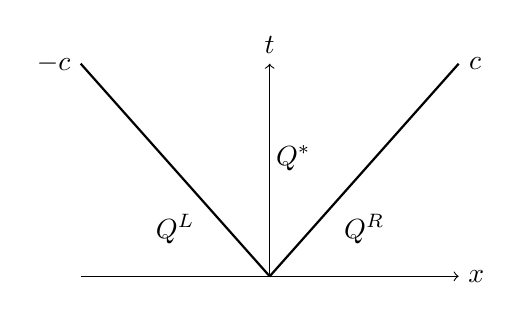
\begin{tikzpicture}[scale=0.6]
  \draw[->] (-4,0) -- (4.,0) node[right] {$x$};
  \draw[->] (0,0) -- (0,4.5) node[above] {$t$};
  \draw[thick] (0,0) -- (4.,4.5) node [right] {$c$};
  \draw[thick] (0,0) -- (-4.,4.5) node [left] {$-c$};
  \node at (2.,1.) {$\vect{Q}^R$};
  \node at (-2.,1.) {$\vect{Q}^L$};
  \node at (0.5,2.5) {$\vect{Q}^*$};
\end{tikzpicture}



%%% Local Variables:
%%% mode: latex
%%% TeX-master: "../../mainManuscript"
%%% End:

  \caption{Solution to Riemann problem \eqref{eq:Riemann_problem} for an elastic bar.}
  \label{fig:elasticity_example}
\end{figure}
Integration of characteristic equations \eqref{eq:elast_charac_equation} respectively along $AP$ and $BP$ yields:
\begin{equation}
  \label{eq:elastic_integral_curves}
  \left\lbrace
    \begin{aligned}
      -& \rho c \(v_P - v_A \) - \(\sigma_P - \sigma_A \) = 0\\
      & \rho c \(v_P - v_B \) - \(\sigma_P - \sigma_B \) = 0
    \end{aligned}
    \right.
\end{equation}
which solution is:
\begin{equation}
  \label{eq:elastic_solution_P}
  v_P = \frac{\sigma_B - \sigma_A}{2\rho c} + \frac{v_A+v_B}{2} \quad ; \quad \sigma_P = \rho c\frac{v_B - v_A}{2} + \frac{\sigma_A+\sigma_B}{2}
\end{equation}
On the other hand, the same procedure for point $P'$ leads to the solution:
\begin{equation}
  \label{eq:elastic_solution_Q}
  v_{P'} = \frac{\sigma_B - \sigma_{A'}}{2\rho c} + \frac{v_{A'}+v_B}{2} \quad ; \quad \sigma_{P'} = \rho c\frac{v_B - v_{A'}}{2} + \frac{\sigma_{A'}+\sigma_B}{2}
\end{equation}
With initial data given for the Riemann problem, it appears that $\Qcb_{A'}=\Qcb_{B}$ and hence, $\Qcb_{P'}=\Qcb_{R} \ne \Qcb_{P}$. Let's assume now that points $P$ and $P'$ are still on each side of the right characteristic straight line emanating from the origin but infinitely close to it. It is obvious that the previous results hold and that the a jump discontinuity propagates in the bar with speed $c$. Hence, we are left with the following condition across a discontinuous wave \cite{Toro} that generalizes to all linear Riemann problems:
\begin{definition}
Given a system of hyperbolic conservation laws $\Qcb_t + \Fcb(\Qcb)_x=\vect{0}$ and a discontinuous wave solution of speed $s_i$ associated to the $i$th characteristic field, the \textbf{Rankine-Hugoniot condition} reads:
\begin{equation}
  \label{eq:rankine-hugoniot}
  \saut{ \Fcb} = s_i \saut{ \Qcb}
\end{equation}
where $\saut{\bullet}$ denotes the jump operator across the discontinuity.  
\end{definition}

\subsubsection*{Characteristic variables -- Waves solution}
Consider a quasi-linear form of dimension $m$ $\Qcb_t + \Jbsf \Qcb_x=\vect{0}$. 
By introducing a set of \textbf{characteristic variables} $\Pcb=\Rbsf^{-1}\Qcb$, where $\Rsf_{ij}=\Rc^j_i$ is the matrix of right eigenvectors, the quasi-linear form of system \eqref{eq:Riemann_problem} can be rewritten in terms of characteristic the variables:
\begin{equation*}
  \begin{aligned}
    &\drond{\Pc_i}{t} + c_i\drond{\Pc_i}{x} = 0 \\
    &\left\lbrace 
      \begin{aligned}
        & \Pc_i(x,t=0) = \Pc_i^L \quad \text{if } x< 0\\
        & \Pc_i(x,t=0) = \Pc_i^R \quad \text{if } x> 0
      \end{aligned}
    \right.
  \end{aligned}
\end{equation*}
with $\Csf_{ij}=c_i\delta_{ij}$, the matrix of eigenvalues so that $\Jsf_{ij} \Rc^j_k = \Rc^k_i\Csf_{kj}$. The solution of this problem is straightforward since it corresponds to a superposition of scalar linear advection equations namely, the initial profil $\Pc_i(x,t=0)$ simply propagates with speed $c_i$ as depicted in figure \ref{fig:advection}. Thus, at a given point $(x,t)$, the solution $\Pc_i(x,t)$ is simply given by tracing backward the characteristic of slope $c_i$ passing through this point to the $x$-axis, that is: $\Pc_i(x,t)=\Pc_i(x-c_it,0)$. 
\begin{figure}[h]
  \centering
  \subfloat{\begin{tikzpicture}[scale=0.75]
  \draw[->] (-4,0) -- (4.,0) node[right] {$x$};
  \draw[->] (0,0) -- (0,4.5) node[above] {$t$};
  \draw[thick] (0,0) -- (4.,4) node [right] {$c_i$};
  % \fill[black] (1.,3.) circle (0.05) node [above] {$P$};
  % \fill[black] (2.10,1.762499) circle (0.05) node [right] {$P'$};
  \draw[dotted] (-4,1.)-- (0,1) node [above left] {$t_1$} --(4.,1);
  \draw[dotted] (-4,2.)-- (0,2) node [above left] {$t_2$} --(4.,2);
  \node[above left] at (0,0) {$t_0$};
\end{tikzpicture}

%%% Local Variables:
%%% mode: latex
%%% TeX-master: "../../mainManuscript"
%%% End:}
  \subfloat{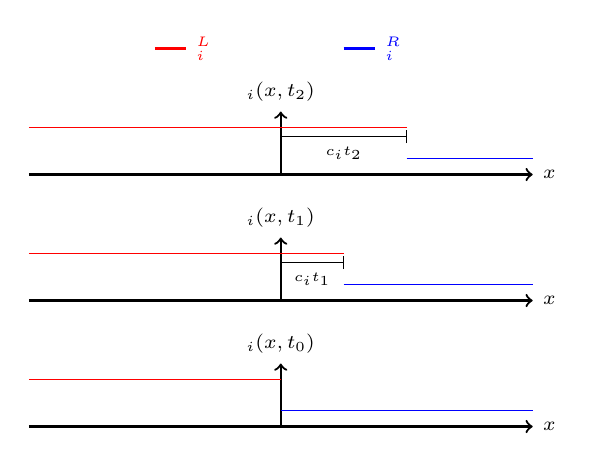
\begin{tikzpicture}[scale=0.8]
  %% t2
  \draw[->,thick] (0,0) -- (0,1) node [above] {\scriptsize$\Pc_i(x,t_2)$};
  \draw[->,thick] (-4,0) -- (4,0) node [right] {\scriptsize$x$};
  \draw[Blue] (2,0.25) -- (4,0.25);
  \draw[Red] (-4,0.75) -- (2,0.75);
  \draw (0,0.6)--(2,0.6) node [midway, below] {\tiny $c_it_2$};
  \draw (2,0.5)--(2,0.7);
  %% t1
  \draw[->,thick] (0,-2) -- (0,-1) node [above] {\scriptsize$\Pc_i(x,t_1)$};
  \draw[->,thick] (-4,-2) -- (4,-2) node [right] {\scriptsize$x$};
  \draw[Blue] (1,0.25-2) -- (4,0.25-2);
  \draw[Red] (-4,0.75-2) -- (1,0.75-2);
  \draw (0,0.6-2)--(1,0.6-2) node [midway, below] {\tiny $c_it_1$};
  \draw (1,0.5-2)--(1,0.7-2);
  %% t0
  \draw[->,thick] (0,-4) -- (0,-3) node [above] {\scriptsize$\Pc_i(x,t_0)$};
  \draw[->,thick] (-4,-4) -- (4,-4) node [right] {\scriptsize$x$};
  \draw[Blue] (0,0.25-4.) -- (4,0.25-4.);
  \draw[Red] (-4,0.75-4.) -- (0,0.75-4.);
  %% legend
  \draw[thick,Red] (-2.,2.) -- (-1.5,2.) node [right] {\scriptsize$\Pc_i^L$};
  \draw[thick,Blue] (1,2.) -- (1.5,2.) node [right] {\scriptsize$\Pc_i^R$};
\end{tikzpicture}
%%% Local Variables:
%%% mode: latex
%%% TeX-master: "../../mainManuscript"
%%% End:}
  \caption{Solution to linear advection equation on the quantity $\Pc_i$ with characteristic speed $c_i$.}
  \label{fig:advection}
\end{figure}
The vector $\Qcb$ is then determined by inverting the relation:
\begin{equation}
  \Qcb = \Rcb^i \Pc_i(x-c_it,0)
\end{equation}
or in terms of the initial data:
\begin{equation}
  \label{eq:Q_expansion}
  \Qcb = \sum_{i=1}^I \Rcb^i \Pc_i^R + \sum_{i=I+1}^m \Rcb^i \Pc_i^L
\end{equation}
where $m$ is $I$ is such that $x-c_I t >0$ and $x-c_{I+1} t <0$. This equation can be seen as an eigenvector expansion of $\Qcb$ with coefficients $\Pc_i^{R,L}$ and in particular:
\begin{equation}
  \label{eq:Qside_expansion}
  \Qcb^L = \sum_{i=1}^{m}\Rcb^i \Pc_i^L \quad ; \quad \Qcb^R = \sum_{i=1}^{m}\Rcb^i \Pc_i^R
\end{equation}
\begin{remark}
  The above discussion highlight the wave nature of the solution to hyperbolic problems. Indeed, since $\Qcb(x,t)$ can be expended into an eigenvector basis with coefficients $\Pc_i$ obeying a linear advection... 
\end{remark}
By rewritting expansion \eqref{eq:Q_expansion}:
\begin{align}
  &\Qcb = \sum_{i=1}^m \Rcb^i \Pc_i^R - \sum_{i=I+1}^m \Rcb^i \(\Pc_i^R - \Pc_i^L\)= \Qcb^R - \sum_{i=I+1}^m \Rcb^i \(\Pc_i^R - \Pc_i^L\) \\
  &\Qcb= \sum_{i=1}^{m}\Rcb^i \Pc_i^L + \sum_{i=1}^I \Rcb^i \(\Pc_i^R - \Pc_i^L\)= \Qcb^L + \sum_{i=1}^I \Rcb^i \(\Pc_i^R - \Pc_i^L\) 
\end{align}
Jump conditions can thus be derived:
\begin{align}
  \label{eq:jump_star_R}
  &  \Qcb-\Qcb^R = -\sum_{i=I+1}^{m} \Rcb^i\delta^i \\
  \label{eq:jump_star_L}
  &  \Qcb-\Qcb^L = \sum_{i=1}^{I} \Rcb^i\delta^i \\
\end{align}
where $\Qcb(x,t)$ is the state lying in the region of the ($x,t$) plane delimited by the $I$th and $(I+1)$th characteristics. In equations \eqref{eq:jump_star_R} and \eqref{eq:jump_star_L}, coefficients $\delta^i=\Pc_i^R - \Pc_i^L$ are called the \textit{wave strengths} and can be computed from \eqref{eq:Qside_expansion} by solving $\Qcb^R-\Qcb^L=\sum_{i=1}^{m}\Rcb^i \delta^i=\Rbsf \vect{\delta}$.

For the linear elastic case considered above, the wave strengths coeeficients are:
\begin{equation}
  \label{eq:elastic_wave_strengths}
  \vect{\delta} = \matrice{\frac{\rho c \(v_B - v_A\) + \(\sigma_B-\sigma_A\)}{2\rho c} \\\frac{\rho c \(v_B - v_A\) - \(\sigma_B-\sigma_A\)}{2\rho c}}
\end{equation}
leading, with equation \eqref{eq:jump_star_L} to:
\begin{equation}
  \label{eq:solution_charac_variables}
  \Qcb = \Qcb^L +\Rcb^1 \delta^1 = \matrice{\frac{\sigma_B - \sigma_A}{2\rho c} + \frac{v_A+v_B}{2} \\ \rho c\frac{v_B - v_A}{2} + \frac{\sigma_A+\sigma_B}{2}} 
\end{equation}
which is the solution found by using the method of characteristics \eqref{eq:elastic_solution_P}.
\subsection{Non-linear problems}
We now consider a hyperelastic medium made of a Saint-Venant-Kirchhoff material, infinite in directions $\vect{e}_2$ and $\vect{e}_3$, and semi-infinite in direction $\vect{e}_1$ (\textit{i.e. $x_1 \in [0,+\infty[$}). This medium suddenly undergoes a load at $(X_1=X=0,t=0)$ in direction $\vect{e}_1$ so that the deformation gradient and the PK1 tensor are respectively:
\begin{align*}
  &\tens{F}=F\vect{e}_1\otimes\vect{e}_1 + \vect{e}_2\otimes\vect{e}_2 + \vect{e}_3\otimes\vect{e}_3 \\
  & \tens{\Pi}=\Pi_{11}\vect{e}_1\otimes\vect{e}_1 + \Pi_{22}\(\vect{e}_2\otimes\vect{e}_2 + \vect{e}_3\otimes\vect{e}_3 \)
\end{align*}
which corresponds to a plane wave solution. We assume that $F(0,t)=\bar{F}$ is given, leading to a \textit{Picard problem} involving both initial and boundary conditions with neglected body forces:
\begin{equation}
  \label{eq:Picard_problem}
  \begin{aligned}
  &\Qcb_t + \drond{\Fcb\cdot \vect{X}}{X_N} = \vect{0}, \\
  &\left\lbrace 
    \begin{aligned}
      & \Qcb(X_N,t=0) = \Qcb^R \quad \text{if } X_N> 0 \\
      & F(0,t) = \bar{F} 
    \end{aligned}
    \right.
  \end{aligned}
\end{equation}
with $\vect{N}=\vect{e}_1$ and:
\begin{equation*}
 \Qcb = \matrice{v \\ F} \quad ; \quad \Fcb = \matrice{-\frac{1}{\rho_0}\Pi \\ -v}
\end{equation*}
where $\Pi=\Pi_{11}$. Since the tangent modulus and the acoustic tensor of Saint-Venant-Kirchhoff model \eqref{eq:SVK_tangent},\eqref{eq:SVK_acoustic} depend on the deformation gradient, the quasi-linear form: $\Qcb_t + \drond{\Fcb}{\Qcb}\drond{\Qcb}{X}=\vect{0}$ is more convenient. The Jacobian matrix is then:
\begin{equation}
  \label{eq:quasi_SVK}
  \Jbsf=\drond{\Fcb}{\Qcb}=-\matrice{0 & -\frac{H_{1111}}{\rho_0} \\ 1 & 0}
\end{equation}
which leads to the characteristic fields:
\begin{equation}
  \label{eq:SVK_charac_fields}
  \left\lbrace
    \begin{aligned}
      & c_1=- \sqrt{\frac{\lambda+2\mu}{2\rho_0}\(3F^2-1\) }\\
      &c_2= \sqrt{\frac{\lambda+2\mu}{2\rho_0}\(3F^2-1\) }
    \end{aligned}\right.
 \quad ; \quad \Lcb^p=\[1\:,\:- c_p \] \quad ; \quad \Rcb^p=\matrice{- c_p \\1} 
\end{equation}
Note that the non-linear flux function (\textit{i.e.} $\ddrond{\Pi_{11}}{F}{F}\neq 0$) yields characteristic fields depending on the strain state and, for the Saint-Venant--Kirchhoff model, possibly complex celerities leading to a loss of hyperbolicity of the problem for $F>\sqrt{\frac{1}{3}}$.

Initial and boundary conditions have an influence on the characteristic structure of the solution due to the dependence of characteristic speeds on the deformation gradient. Indeed, if initial data are given so that $\bar{F} > F_R$, the resulting characteristic speeds satisfy $c_2(\bar{F})>c_2(F_R)$ leading to characteristics colliding in the right region of the ($x,t$) plane (figure \ref{fig:Picard_problem}\subref{subfig:2S}). On the other hand, $\bar{F} < F_R$ yields characteristic moving away from each other in the right region according to $c_2(\bar{F})<c_2(F_R)$ (figure \ref{fig:Picard_problem}\subref{subfig:2R}). Those two situations, respectively corresponding to a shock wave and a simple wave, will be studied in what follows.
\begin{figure}[h]
  \centering
  \subfloat[Right-going shock wave\label{subfig:2S}]{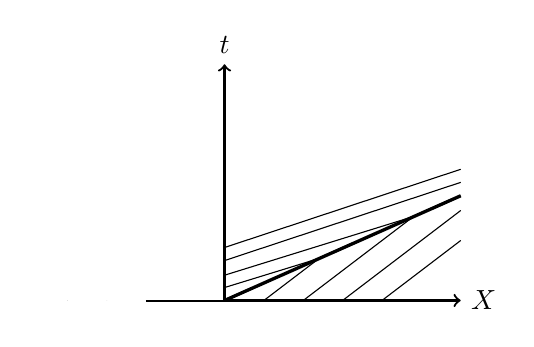
\begin{tikzpicture}
  \draw[->,thick] (-1,0) -- (3,0) node[right] {$X$};
  \draw[->,thick](0,0) -- (0,3) node[above] {$t$};
  \draw(-0.5,0.01) -- (1.20,0.533333) ;
  \draw(-1,0.01) -- (2.40,1.066) ;
  \draw(-1.5,0.01) -- (3,1.5) ;
  \draw(-2,0.01) -- (3,1.666) ;
  %%%%%%%%% 
  \draw(0.5,0) -- (1.20,0.533333) ;
  \draw(1.,0) -- (2.40,1.066) ;
  \draw(1.5,0) -- (3,1.14285) ;
  \draw(2.0,0) -- (3,0.7619) ;
  \draw[very thick] (0,0) -- (3,1.33);
  \fill[white] (-2.5,2.5) rectangle (-0.015,0.01);
  \fill[white] (-2.,0) rectangle (-1.,0.1);
\end{tikzpicture}}
  \subfloat[Right-going simple wave\label{subfig:2R}]{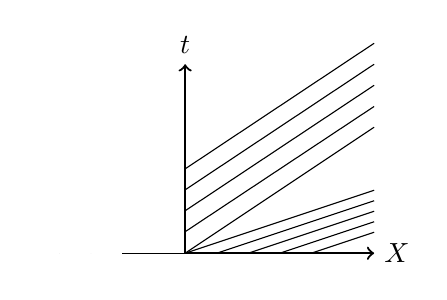
\begin{tikzpicture}[scale=0.8]
  \draw[->,thick] (-1,0) -- (3,0) node[right] {$X$};
  \draw[->,thick](0,0) -- (0,3) node[above] {$t$};
  \draw(0,0) -- (3,2) ;
  \draw(-0.5,0.01) -- (3,2.33) ;
  \draw(-1,0.01) -- (3,2.666) ;
  \draw(-1.5,0.01) -- (3,3) ;
  \draw(-2,0.01) -- (3,3.333) ;
  \draw(0,0) -- (3,1) ;
  \draw(0.5,0) -- (3,0.833) ;
  \draw(1,0) -- (3,0.666) ;
  \draw(1.5,0) -- (3,0.5) ;
  \draw(2,0) -- (3,0.333);
  \fill[white] (-2.5,2.5) rectangle (-0.015,0.01);
  \fill[white] (-2.,0) rectangle (-1.,0.1);
\end{tikzpicture}}
  \caption{Solutions to Picard problem \eqref{eq:Picard_problem} depending on initial and boundary data.}
  \label{fig:Picard_problem}
\end{figure}

\subsubsection*{Shock waves}
By applying the method of characteristics between the $x$-axis and an intersection point of two characteristic straight lines allows to show that a shock wave carry a jump discontinuity of the conserved quantity vector and hence, satisfy the Rankine-Hugoniot condition \eqref{eq:rankine-hugoniot} where the shock speed $s_i$ is to be defined. According to Rankine-Hugoniot conditions, those states obey:
\begin{align}
  \label{eq:RH_velocity}
  & -\frac{1}{\rho_0}\(\bar{\Pi} - \Pi_R \) = s \( \bar{v} - v_R \)\\
  \label{eq:RH_F}
  & - \( \bar{v}-v_R\)=s\( \bar{F} - F_R\)
\end{align}
For the sake of generality, $\bar{F}$ is considered as an unknown so that a relation connecting $\Qcb^R$ to a set of solutions $\Qcb$ through a shock wave can be developed.

Substitution of $s$ from equation \eqref{eq:RH_F} and introduction in equation \eqref{eq:RH_velocity} where $\Pi=\frac{\lambda+2\mu}{2}\(F^3-F\)$ yield:
\begin{align}
  \label{eq:shock_speed}
  & s=-\frac{v-v_R}{F - F_R}\\
  \label{eq:v_jump}
  & v-v_R= \pm \sqrt{\frac{\lambda+2\mu}{2\rho_0}(F-F_R)\[ F^3-F - (F_R^3-F_R)\]}
\end{align}
In addition to the Rankine-Hugoniot condition, the \textit{Lax entropy condition} stating that characteristic curves collide in a shock wave must be satisfied \cite[p.268]{Leveque}:
\begin{equation}
  \label{eq:Lax_entropy}
  \lambda(F)<s<\lambda(F_R)
\end{equation}
For a Saint-Venant--Kirchhoff material, the Lax condition leads to $F > F_R$ ensuring thus that the square root in equation \eqref{eq:v_jump} is real.


Equation \eqref{eq:v_jump} yields two families of curves in the phase plane, one of which is expected to identify with the jump conditions derived for the linear case \eqref{eq:jump_star_R} when considering an infinitesimal jump (\textit{i.e. $F=F_R+\epsilon$ with $\epsilon \rightarrow 0$}). Thus, equation \eqref{eq:v_jump} reads:
\begin{equation}
  \label{eq:linearization}
  v-v_R= \pm \sqrt{\frac{\lambda+2\mu}{2\rho_0}\epsilon\[ (F_R+\epsilon)^3-(F_R+\epsilon) - (F_R^3-F_R)\]}
\end{equation}
where, with $\epsilon \rightarrow 0$:
\begin{equation*}
  (F_R+\epsilon)^3\approx F_R^3(1+\frac{3\epsilon}{F_R})
\end{equation*}
and hence,
\begin{equation*}
  \matrice{v \\ F}=\matrice{v_R \\ F_R} + \epsilon \matrice{1 \\\pm \sqrt{\frac{\lambda+2\mu}{2\rho_0}\[ 3F_R^2-1\]}}
\end{equation*}
Hence, the \textit{minus} sign yields the linearized expression \eqref{eq:jump_star_R} for a right-going shock, the \textit{plus} sign holds, on the other hand, for left-going shocks. Finally, the Rankine-Hugoniot condition across a left-going shock and a right-going shock respectively yields:
\begin{align}
  \label{eq:left-going_shock}
  &v-v_L= \sqrt{\frac{\lambda+2\mu}{2\rho_0}(F-F_L)\[ F^3-F - (F_L^3-F_L)\]} \\
  \label{eq:right-going_shock}
  &v-v_R= -\sqrt{\frac{\lambda+2\mu}{2\rho_0}(F-F_R)\[ F^3-F - (F_R^3-F_R)\]}
\end{align}

\subsubsection*{Simple waves}
In order to study the evolution of fields within the void region in figure \ref{fig:Picard_problem}\subref{subfig:2R}, let's write the left-going characteristic equation through it with $\Lcb^1=[1,-c_1]$:
\begin{equation}
  \label{eq:SVK_rarefaction}
  dv -c_1  dF = 0 %+\sqrt{\frac{\lambda + 2\mu}{2\rho_0}\(3F^2-1\)}
\end{equation}

\begin{remark}
  If one was seeking a similarity solution in this region, the conserved quantity vector would be looked for so that $\Qcb'(x/t)$ is proportional to the right eigenvector $\Rcb^2$ asrequired by equation \eqref{eq:quasi-linear_similarity}. By denoting the ray $\xi=x/t$, this proportionality condition is:
  \begin{equation*}
    \matrice{\ddroit{v}{\xi} \\ \ddroit{F}{\xi}} = \matrice{ -c_2 \\ 1}
  \end{equation*}
  Combining these equations and noting that $c_2=-c_1$ allows to recover equation \eqref{eq:SVK_rarefaction}:
  \begin{equation}
    \label{eq:rarefaction}
    \begin{aligned}
      & dv -c_1 d\xi = 0\\
      & dF = d\xi
    \end{aligned}
  \end{equation}
Hence, the structure depicted in figure \ref{fig:Picard_problem}\subref{subfig:2R} corresponds to a rarefaction wave. Fields evolve smoothly within the void region according to equations \eqref{eq:rarefaction}, leading to a characteristic fan since $c_2=c_2(F)$ and $F$ decreases from $F_R$ to $\bar{F}$.
\end{remark}


As for shock waves, the complete set of states $\Qcb$ connected to $\Qcb^R$ through a rarefaction wave will be derived. To do so, the following change of variable is introduced: $F \mapsto ch(x)/\sqrt{3}$, so that equation \eqref{eq:SVK_rarefaction} becomes:
\begin{equation}
  \label{eq:charac_equation_sh}
  dv=-\sqrt{\frac{\lambda + 2\mu}{6\rho_0}}sh(x)^2 dx
\end{equation}
where, the hyperbolic cosine $ch(x)$ and sine $sh(x)$ satisfy: $ch(x)^2-sh(x)^2=1$. Equation \eqref{eq:charac_equation_sh} can be easily integrated with the exponential form of hyperbolic sine: $sh(x)=\frac{e^x - e^{-x}}{2}$. Thus, one gets:
\begin{equation*}
  v-v_R=-\frac{1}{4}\sqrt{\frac{\lambda + 2\mu}{6\rho_0}}\[sh(2x)-2x -(sh(2x_R)-2x_R)\]
\end{equation*}
At last, the inverse change of variable:
\begin{align*}
  &sh(2x)=2ch(x)sh(x)=2\sqrt{3}F\sqrt{3F^2-1} \\
  &2x=2\arg\(ch(\sqrt{3}F)\)=2\ln\(\sqrt{3}F + \sqrt{3F^2-1}\)
\end{align*}
yields the relation:
\begin{equation}
  \label{eq:integral_curve_right}
  v-v_R=-\sqrt{\frac{\lambda + 2\mu}{24\rho_0}}\[\sqrt{3}\(F\sqrt{3F^2-1} -F_R\sqrt{3F_R^2-1}\)-\ln\(\frac{\sqrt{3}F + \sqrt{3F^2-1}}{\sqrt{3}F_R + \sqrt{3F_R^2-1}}\) \]
\end{equation}
In a similar manner, the following condition must hold through a left-going rarefaction wave:
\begin{equation*}
  dv -c_2  dF = 0
\end{equation*}
which leads to:
\begin{equation}
  \label{eq:integral_curve_left}
  v-v_L=\sqrt{\frac{\lambda + 2\mu}{24\rho_0}}\[\sqrt{3}\(F\sqrt{3F^2-1} -F_L\sqrt{3F_L^2-1}\)-\ln\(\frac{\sqrt{3}F + \sqrt{3F^2-1}}{\sqrt{3}F_L + \sqrt{3F_L^2-1}}\) \]
\end{equation}



\subsubsection*{Solution to the Riemann problem}
Now the solution to Picard's problems have been derived, the solution to the Riemann problem can be developed. Once again, the problem is formulated as:
\begin{equation}
  \begin{aligned}
    &\Qcb_t + \drond{\Fcb\cdot \vect{N}}{X_N} = \vect{0}, \\
    &\left\lbrace 
      \begin{aligned}
        & \Qcb(X_N,t=0) = \Qcb^L \quad \text{if } X_N< 0\\
        & \Qcb(X_N,t=0) = \Qcb^R \quad \text{if } X_N> 0
      \end{aligned}
    \right.
  \end{aligned}
\end{equation}
As for the Picard problem, initial conditions influence the characteristic structure of the solution. Indeed, if initial conditions are given such that $F_L<F_R$, left-going characteristics will collide while right-going ones will move away from one another (see figure \ref{fig:RP_solution}\subref{subfig:1S2R}). In that case, the first and second characteristic fields will respectively be refered to as a \textit{1-shock} and a \textit{2-rarefaction}. Conversely, if $F_L>F_R$, the solution will correspond to a \textit{1-rarefaction} and a \textit{2-shock} (figure \ref{fig:RP_solution}\subref{subfig:1R2S}). 

\begin{figure}[h]
  \centering
  \subfloat[$F_L < F_R$\label{subfig:1S2R}]{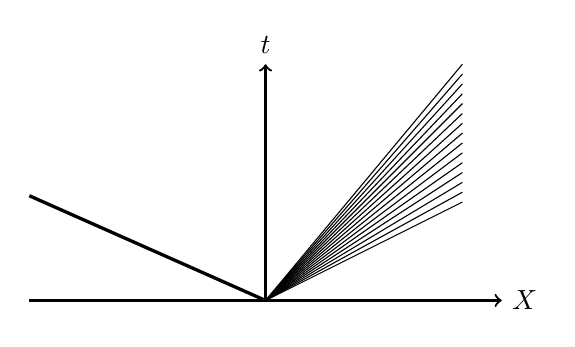
\begin{tikzpicture}
  \draw[->,thick] (-3,0) -- (3,0) node[right] {$X$};
  \draw[->,thick](0,0) -- (0,3) node[above] {$t$};
  %% Shock wave
  \draw[very thick] (0,0) -- (-3,1.33);
  %% Rarefaction wave
  \foreach \x in {0.5,0.55,...,1.25}
  \draw(0,0) -- (2.5,2.5*\x) ;
\end{tikzpicture}}
  \subfloat[$F_L > F_R$\label{subfig:1R2S}]{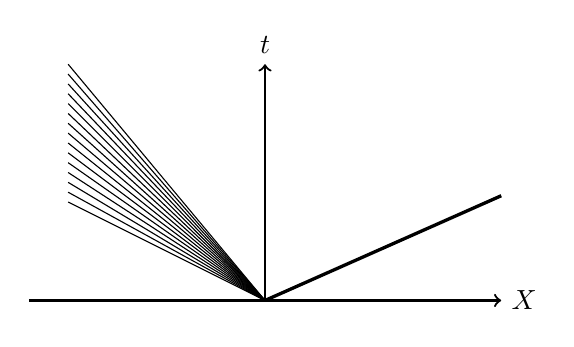
\begin{tikzpicture}
  \draw[->,thick] (-3,0) -- (3,0) node[right] {$X$};
  \draw[->,thick](0,0) -- (0,3) node[above] {$t$};
  %% Shock wave
  \draw[very thick] (0,0) -- (3,1.33);
  %% Rarefaction wave
  \foreach \x in {0.5,0.55,...,1.25}
  \draw(0,0) -- (-2.5,2.5*\x) ;
\end{tikzpicture}}
  \caption{General wave patterns arrising in the solution to Riemann problem depending on intial data. (a): 1-shock, 2-rarefaction. (b): 1-rarefaction, 2-shock.}
  \label{fig:RP_solution}
\end{figure}

For the 1-shock,2-rarefaction solution one then seeks a state $\Qcb^*$ that is connected to $\Qcb^L$ and $\Qcb^R$ through respectively a shock wave and a rarefaction wave. Hence, $\Qcb^*$ must satisfy equations \eqref{eq:left-going_shock} and \eqref{eq:integral_curve_right}, namely:
\begin{equation}
  \label{eq:1S2R_solution}
  \left\lbrace
  \begin{aligned}
    &v_*-v_L= \sqrt{\frac{\lambda+2\mu}{2\rho_0}(F_*-F_L)\[ F_*^3-F_* - (F_L^3-F_L)\]} \\
    &v_*-v_R=-\sqrt{\frac{\lambda + 2\mu}{24\rho_0}}\[\sqrt{3}\(F_*\sqrt{3F_*^2-1} -F_R\sqrt{3F_R^2-1}\)-\ln\(\frac{\sqrt{3}F_* + \sqrt{3F_*^2-1}}{\sqrt{3}F_R + \sqrt{3F_R^2-1}}\) \]
  \end{aligned}
  \right.
\end{equation}
Analogously, the 1-rarefaction,2-shock solution is given by the solution of equations \eqref{eq:integral_curve_left} and \eqref{eq:right-going_shock}:
\begin{equation}
  \label{eq:1R2S_solution}
  \left\lbrace
  \begin{aligned}
    &v_*-v_L=\sqrt{\frac{\lambda + 2\mu}{24\rho_0}}\[\sqrt{3}\(F_*\sqrt{3F_*^2-1} -F_L\sqrt{3F_L^2-1}\)-\ln\(\frac{\sqrt{3}F_* + \sqrt{3F_*^2-1}}{\sqrt{3}F_L + \sqrt{3F_L^2-1}}\) \]\\
    &v_*-v_R= -\sqrt{\frac{\lambda+2\mu}{2\rho_0}(F_*-F_R)\[ F_*^3-F_* - (F_R^3-F_R)\]}
  \end{aligned}
  \right.
\end{equation}
Once one of this system is solved, the solution $\Qcb$ is known everywhere except inside the rarefaction fan. Nevertheless, in this region $\Qcb$ only varies with the ray $\xi=c_i(F)$ and hence, the solution inside an $i$-rarefaction wave satisfies:
\begin{equation}
  \label{eq:rarefaction_fan}
  \xi = \pm \sqrt{\frac{\lambda + 2\mu}{2\rho_0}\(3F^2-1 \)} \quad \Rightarrow \quad F(\xi)= \sqrt{\frac{2\rho_0}{3(\lambda + 2\mu)}\xi^2-1}
\end{equation}
\begin{figure}[h]
  \centering
  \subfloat[Initial data: $F_L=1 ; F_R=2$ \label{subfig:1S2R_curves}]{\definecolor{Purple}{RGB}{120,28,129}
\definecolor{Blue}{RGB}{63,96,174}
\definecolor{Duck}{RGB}{83,158,182}
\definecolor{Green}{RGB}{109,179,136}
\definecolor{Yellow}{RGB}{202,184,67}
\definecolor{Orange}{RGB}{231,133,50}
\definecolor{Red}{RGB}{217,33,32}
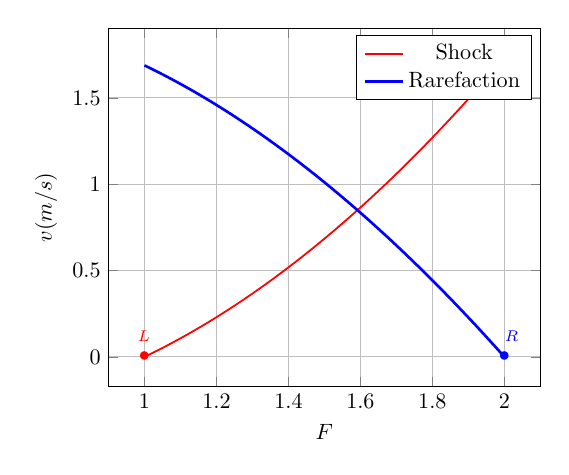
\begin{tikzpicture}[scale=0.8]
\begin{axis}[xlabel=$F$,ylabel=$v (m/s)$,ymajorgrids=true,xmajorgrids=true]
  \addplot[Red,thick] coordinates {(1.0,0.0) (1.0196019601960196,0.019889905868838792) (1.0392039203920391,0.04035480171519238) (1.058805880588059,0.06139339246981025) (1.0784078407840785,0.08300445472552491) (1.098009800980098,0.1051868317293367) (1.1176117611761176,0.1279394287977403) (1.1372137213721372,0.1512612091133456) (1.1568156815681567,0.17515118986560513) (1.1764176417641765,0.19960843870261852) (1.196019601960196,0.2246320704646163) (1.2156215621562156,0.25022124417291264) (1.2352235223522352,0.2763751602509047) (1.2548254825482548,0.30309305795616337) (1.2744274427442743,0.330374213004825) (1.2940294029402941,0.3582179353714115) (1.3136313631363137,0.386623567248899) (1.3332333233323332,0.4155904811553686) (1.3528352835283528,0.445118078174895) (1.3724372437243724,0.47520578632153143) (1.3920392039203922,0.5058530590163028) (1.4116411641164117,0.5370593736680643) (1.4312431243124313,0.568824230349938) (1.4508450845084508,0.6011471505637854) (1.4704470447044704,0.6340276760858663) (1.4900490049004902,0.667465367887438) (1.5096509650965095,0.7014598051246006) (1.5292529252925293,0.7360105841921958) (1.5488548854885489,0.7711173178369951) (1.5684568456845684,0.8067796343258441) (1.5880588058805882,0.8429971766647708) (1.6076607660766076,0.8797696018654025) (1.6272627262726274,0.917096580255355) (1.646864686468647,0.9549777948294852) (1.6664666466646665,0.9934129406392047) (1.686068606860686,1.032401724217221) (1.7056705670567056,1.0719438630353144) (1.7252725272527254,1.1120390849929296) (1.7448744874487447,1.1526871279345328) (1.7644764476447645,1.1938877391938512) (1.784078407840784,1.2356406751632294) (1.8036803680368036,1.2779457008865038) (1.8232823282328234,1.320802589673878) (1.8428842884288428,1.3642111227374165) (1.8624862486248626,1.4081710888458763) (1.8820882088208821,1.4526822839976499) (1.9016901690169017,1.4977445111107466) (1.9212921292129215,1.543357579728744) (1.9408940894089408,1.5895213057417645) (1.9604960496049606,1.6362355111215798) (1.9800980098009802,1.6835000236699957) (1.9996999699969997,1.7313146767797576) };
  \addplot[Blue,very thick] coordinates {(1.0,1.6884673989302577) (1.0196019601960196,1.6685781823289632) (1.0392039203920391,1.648117983645035) (1.058805880588059,1.6270917763366024) (1.0784078407840785,1.6055041425368688) (1.098009800980098,1.5833593157699348) (1.1176117611761176,1.5606612177002648) (1.1372137213721372,1.5374134899261505) (1.1568156815681567,1.5136195216278194) (1.1764176417641765,1.48928247372591) (1.196019601960196,1.4644053000848238) (1.2156215621562156,1.4389907661996928) (1.2352235223522352,1.4130414657294894) (1.2548254825482548,1.3865598351776642) (1.2744274427442743,1.3595481669723095) (1.2940294029402941,1.3320086211576845) (1.3136313631363137,1.3039432358761032) (1.3332333233323332,1.2753539367920979) (1.3528352835283528,1.246242545588463) (1.3724372437243724,1.216610787645106) (1.3920392039203922,1.1864602989961286) (1.4116411641164117,1.1557926326474621) (1.4312431243124313,1.12460926432638) (1.4508450845084508,1.092911597724879) (1.4704470447044704,1.0607009692909792) (1.4900490049004902,1.0279786526152188) (1.5096509650965095,0.994745862453826) (1.5292529252925293,0.9610037584250569) (1.5488548854885489,0.9267534484108921) (1.5684568456845684,0.8919959916925568) (1.5880588058805882,0.8567324018451127) (1.6076607660766076,0.8209636494135533) (1.6272627262726274,0.7846906643903794) (1.646864686468647,0.7479143385125069) (1.6664666466646665,0.7106355273934435) (1.686068606860686,0.6728550525050632) (1.7056705670567056,0.6345737030218022) (1.7252725272527254,0.595792237538853) (1.7448744874487447,0.5565113856747698) (1.7644764476447645,0.5167318495678894) (1.784078407840784,0.47645430527509447) (1.8036803680368036,0.43567940408061234) (1.8232823282328234,0.3944077737218566) (1.8428842884288428,0.3526400195386741) (1.8624862486248626,0.31037672555176576) (1.8820882088208821,0.2676184554755838) (1.9016901690169017,0.22436575367049583) (1.9212921292129215,0.18061914603862234) (1.9408940894089408,0.13637914086738703) (1.9604960496049606,0.09164622962443836) (1.9800980098009802,0.04642088770736517) (1.9996999699969997,0.0007035751512764867) };
  \node at (axis cs:1,0) [Red] {$\bullet$};
  \node at (axis cs:2.,0) [Blue] {$\bullet$};
  % \node[coordinate] at (axis cs:1.,0.) {$Mich$};
  \node at (axis cs:1,0) [anchor=south,Red] {$\Qcb^L$};
  \node at (axis cs:1.98,0) [above right,Blue] {$\Qcb^R$};
  \legend{Shock,Rarefaction}
  % \addplot[Blue,dashed,very thick,domain=1:2,samples=51,samples y=0]
  %   ({x},{0.-sqrt(0.5*(12.-1))*(x-2.)});
  % \addplot[Red,dashed,very thick,domain=1:2,samples=51,samples y=0]
  %   ({x},{0.+sqrt(0.5*(2.-1))*(x-1.)});
\end{axis}
\end{tikzpicture}
}
  \subfloat[Initial data: $F_L=2 ; F_R=1$ \label{subfig:1S2R_curves}]{\definecolor{Purple}{RGB}{120,28,129}
\definecolor{Blue}{RGB}{63,96,174}
\definecolor{Duck}{RGB}{83,158,182}
\definecolor{Green}{RGB}{109,179,136}
\definecolor{Yellow}{RGB}{202,184,67}
\definecolor{Orange}{RGB}{231,133,50}
\definecolor{Red}{RGB}{217,33,32}
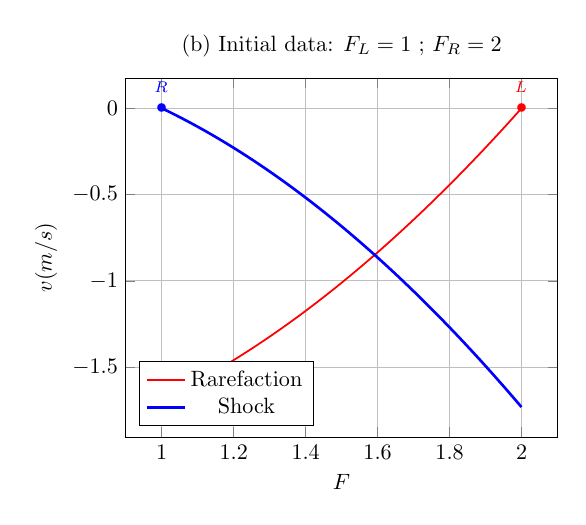
\begin{tikzpicture}[scale=0.8]
\begin{axis}[xlabel=$F$,ylabel=$v (m/s)$,ymajorgrids=true,xmajorgrids=true,legend pos=south west,title={(b) Initial data: $F_L=1$ ; $F_R=2$}]
  \addplot[Red,thick] coordinates {(1.0,-1.6884673989302577) (1.0196019601960196,-1.6685781823289632) (1.0392039203920391,-1.648117983645035) (1.058805880588059,-1.6270917763366024) (1.0784078407840785,-1.6055041425368688) (1.098009800980098,-1.5833593157699348) (1.1176117611761176,-1.5606612177002648) (1.1372137213721372,-1.5374134899261505) (1.1568156815681567,-1.5136195216278194) (1.1764176417641765,-1.48928247372591) (1.196019601960196,-1.4644053000848238) (1.2156215621562156,-1.4389907661996928) (1.2352235223522352,-1.4130414657294894) (1.2548254825482548,-1.3865598351776642) (1.2744274427442743,-1.3595481669723095) (1.2940294029402941,-1.3320086211576845) (1.3136313631363137,-1.3039432358761032) (1.3332333233323332,-1.2753539367920979) (1.3528352835283528,-1.246242545588463) (1.3724372437243724,-1.216610787645106) (1.3920392039203922,-1.1864602989961286) (1.4116411641164117,-1.1557926326474621) (1.4312431243124313,-1.12460926432638) (1.4508450845084508,-1.092911597724879) (1.4704470447044704,-1.0607009692909792) (1.4900490049004902,-1.0279786526152188) (1.5096509650965095,-0.994745862453826) (1.5292529252925293,-0.9610037584250569) (1.5488548854885489,-0.9267534484108921) (1.5684568456845684,-0.8919959916925568) (1.5880588058805882,-0.8567324018451127) (1.6076607660766076,-0.8209636494135533) (1.6272627262726274,-0.7846906643903794) (1.646864686468647,-0.7479143385125069) (1.6664666466646665,-0.7106355273934435) (1.686068606860686,-0.6728550525050632) (1.7056705670567056,-0.6345737030218022) (1.7252725272527254,-0.595792237538853) (1.7448744874487447,-0.5565113856747698) (1.7644764476447645,-0.5167318495678894) (1.784078407840784,-0.47645430527509447) (1.8036803680368036,-0.43567940408061234) (1.8232823282328234,-0.3944077737218566) (1.8428842884288428,-0.3526400195386741) (1.8624862486248626,-0.31037672555176576) (1.8820882088208821,-0.2676184554755838) (1.9016901690169017,-0.22436575367049583) (1.9212921292129215,-0.18061914603862234) (1.9408940894089408,-0.13637914086738703) (1.9604960496049606,-0.09164622962443836) (1.9800980098009802,-0.04642088770736517) (1.9996999699969997,-0.0007035751512764867) };
  \addplot[Blue,very thick] coordinates {(1.0,0.0) (1.0196019601960196,-0.019889905868838792) (1.0392039203920391,-0.04035480171519238) (1.058805880588059,-0.06139339246981025) (1.0784078407840785,-0.08300445472552491) (1.098009800980098,-0.1051868317293367) (1.1176117611761176,-0.1279394287977403) (1.1372137213721372,-0.1512612091133456) (1.1568156815681567,-0.17515118986560513) (1.1764176417641765,-0.19960843870261852) (1.196019601960196,-0.2246320704646163) (1.2156215621562156,-0.25022124417291264) (1.2352235223522352,-0.2763751602509047) (1.2548254825482548,-0.30309305795616337) (1.2744274427442743,-0.330374213004825) (1.2940294029402941,-0.3582179353714115) (1.3136313631363137,-0.386623567248899) (1.3332333233323332,-0.4155904811553686) (1.3528352835283528,-0.445118078174895) (1.3724372437243724,-0.47520578632153143) (1.3920392039203922,-0.5058530590163028) (1.4116411641164117,-0.5370593736680643) (1.4312431243124313,-0.568824230349938) (1.4508450845084508,-0.6011471505637854) (1.4704470447044704,-0.6340276760858663) (1.4900490049004902,-0.667465367887438) (1.5096509650965095,-0.7014598051246006) (1.5292529252925293,-0.7360105841921958) (1.5488548854885489,-0.7711173178369951) (1.5684568456845684,-0.8067796343258441) (1.5880588058805882,-0.8429971766647708) (1.6076607660766076,-0.8797696018654025) (1.6272627262726274,-0.917096580255355) (1.646864686468647,-0.9549777948294852) (1.6664666466646665,-0.9934129406392047) (1.686068606860686,-1.032401724217221) (1.7056705670567056,-1.0719438630353144) (1.7252725272527254,-1.1120390849929296) (1.7448744874487447,-1.1526871279345328) (1.7644764476447645,-1.1938877391938512) (1.784078407840784,-1.2356406751632294) (1.8036803680368036,-1.2779457008865038) (1.8232823282328234,-1.320802589673878) (1.8428842884288428,-1.3642111227374165) (1.8624862486248626,-1.4081710888458763) (1.8820882088208821,-1.4526822839976499) (1.9016901690169017,-1.4977445111107466) (1.9212921292129215,-1.543357579728744) (1.9408940894089408,-1.5895213057417645) (1.9604960496049606,-1.6362355111215798) (1.9800980098009802,-1.6835000236699957) (1.9996999699969997,-1.7313146767797576) };
  \node at (axis cs:1,0) [Blue] {$\bullet$};
  \node at (axis cs:2.,0) [Red] {$\bullet$};
  \node at (axis cs:1,0) [anchor=south,Blue] {$\Qcb^R$};
  \node at (axis cs:2,0) [anchor=south,Red] {$\Qcb^L$};
\legend{Rarefaction,Shock}
\end{axis}
\end{tikzpicture}
}
  \caption{Set of connected states $\Qcb$ to initial data through shock and rarefaction waves with $v_L=v_R=0$ in both cases: (a) 1-shock,2-rarefaction solution ; (b) 1-rarefaction, 2-shock.}
  \label{fig:solutions_RP}
\end{figure}


\begin{remark}
  The above discussion holds for concave flux functions which is not the case for the neo-Hookean model for instance. Indeed, such a model yields a monotonically decreasing positive characteristic speeds with the gradient of deformation (see figure \ref{fig:SVK-NH}\subref{subfig:SVK_NH_speeds}). Hence, initial data considered previously will lead to opposite situations (\textit{i.e. $F_L<F_R \rightarrow $ 1--rarefaction ; 2--shock, and $F_L>F_R \rightarrow $ 1--shock ; 2--rarefaction}). Moreover, the polyconvexity of the neo-Hookean stored energy function ensures the hyperbolicity of the system so that the problem does not suffer any limitation on the deformation gradient.
  \begin{figure}[h]
    \centering
    \subfloat[Stress $\Pi_{11}$ \label{subfig:SVK_NH_Pi}]{\definecolor{Red}{RGB}{217,33,32}
\definecolor{Blue}{RGB}{63,96,174}
\definecolor{Duck}{RGB}{83,158,182}
\definecolor{Green}{RGB}{109,179,136}
\definecolor{Yellow}{RGB}{202,184,67}
\definecolor{Orange}{RGB}{231,133,50}
\definecolor{Red}{RGB}{217,33,32}
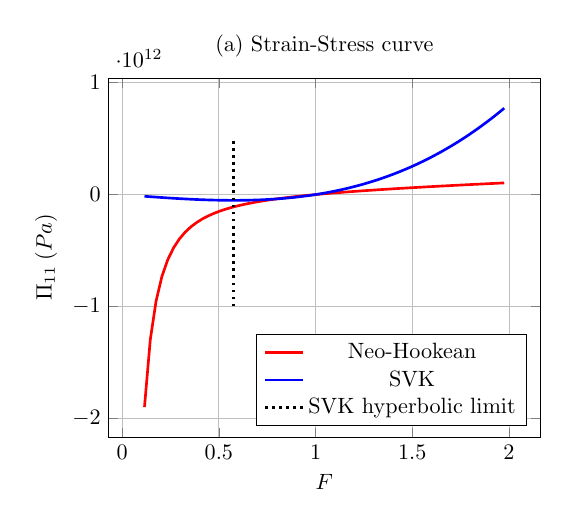
\begin{tikzpicture}[scale=0.8]
\begin{axis}[xlabel=$F$,ylabel=$\Pi_{11} \: (Pa)$,ymajorgrids=true,xmajorgrids=true,legend pos=south east,title={(a) Strain-Stress curve}]
\addplot[Red,very thick] coordinates {(0.11547005383792518,-1898966453319.162) (0.14547005383792516,-1296837707486.0405) (0.17547005383792513,-951312235719.5623) (0.20547005383792513,-732355105152.6451) (0.23547005383792513,-583575852118.2125) (0.2654700538379251,-477087968993.8754) (0.2954700538379251,-397729449724.4541) (0.3254700538379251,-336642141070.28204) (0.35547005383792507,-288349957545.72546) (0.38547005383792504,-249309520683.61847) (0.415470053837925,-217140040714.9308) (0.44547005383792504,-190190468824.5224) (0.475470053837925,-167284549773.97247) (0.505470053837925,-147564580724.34894) (0.535470053837925,-130392343185.27245) (0.5654700538379249,-115284401045.16144) (0.595470053837925,-101868733030.67676) (0.625470053837925,-89854990617.66492) (0.6554700538379249,-79013679521.07468) (0.6854700538379249,-69161318053.14328) (0.7154700538379248,-60149680216.69014) (0.7454700538379249,-51857881714.88495) (0.7754700538379249,-44186477584.150566) (0.8054700538379248,-37053004869.531456) (0.8354700538379248,-30388577783.986546) (0.8654700538379249,-24135259235.847366) (0.8954700538379248,-18244011798.887867) (0.9254700538379248,-12673085866.843775) (0.9554700538379248,-7386740998.494719) (0.9854700538379247,-2354223588.251995) (1.0154700538379247,2451056537.9352818) (1.0454700538379247,7052193879.264957) (1.0754700538379247,11469332294.041113) (1.1054700538379247,15720112571.176903) (1.1354700538379248,19820042073.450085) (1.1654700538379246,23782801671.8228) (1.1954700538379246,27620501912.14364) (1.2254700538379246,31343897846.142628) (1.2554700538379246,34962570023.63762) (1.2854700538379247,38485077640.53793) (1.3154700538379245,41919088663.206696) (1.3454700538379245,45271490826.59238) (1.3754700538379245,48548486673.378265) (1.4054700538379246,51755675220.64049) (1.4354700538379246,54898122376.10795) (1.4654700538379246,57980421852.87309) (1.4954700538379244,61006748029.95563) (1.5254700538379244,63980901961.52675) (1.5554700538379245,66906351538.24785) (1.5854700538379245,69786266641.0072) (1.6154700538379245,72623549993.23035) (1.6454700538379243,75420864307.28705) (1.6754700538379244,78180656228.87244) (1.7054700538379244,80905177507.05946) (1.7354700538379244,83596503754.174) (1.7654700538379244,86256551106.45828) (1.7954700538379245,88887091051.8295) (1.8254700538379243,91489763653.42323) (1.8554700538379243,94066089365.83081) (1.8854700538379243,96617479614.0105) (1.9154700538379243,99145246281.97147) (1.9454700538379244,101650610238.83322) (1.9754700538379242,104134709013.2085) };
\addplot[Blue,very thick] coordinates {(0.11547005383792518,-15336791766.165447) (0.14547005383792516,-19168111304.289738) (0.17547005383792513,-22893685303.277996) (0.20547005383792513,-26491706070.822536) (0.23547005383792513,-29940365914.61566) (0.2654700538379251,-33217857142.349674) (0.2954700538379251,-36302372061.71689) (0.3254700538379251,-39172102980.40962) (0.35547005383792507,-41805242206.12016) (0.38547005383792504,-44179982046.540825) (0.415470053837925,-46274514809.36392) (0.44547005383792504,-48067032802.28176) (0.475470053837925,-49535728332.98665) (0.505470053837925,-50658793709.17089) (0.535470053837925,-51414421238.526794) (0.5654700538379249,-51780803228.74666) (0.595470053837925,-51736131987.522804) (0.625470053837925,-51258599822.54755) (0.6554700538379249,-50326399041.513176) (0.6854700538379249,-48917721952.112) (0.7154700538379248,-47010760862.036354) (0.7454700538379249,-44583708078.97849) (0.7754700538379249,-41614755910.630775) (0.8054700538379248,-38082096664.68549) (0.8354700538379248,-33963922648.83495) (0.8654700538379249,-29238426170.77144) (0.8954700538379248,-23883799538.187305) (0.9254700538379248,-17878235058.774815) (0.9554700538379248,-11199925040.226295) (0.9854700538379247,-3827061790.2340784) (1.0154700538379247,4262162383.5095387) (1.0454700538379247,13089555173.312326) (1.0754700538379247,22676924271.481888) (1.1054700538379247,33046077370.32594) (1.1354700538379248,44218822162.15218) (1.1654700538379246,56216966339.268196) (1.1954700538379246,69062317593.98189) (1.2254700538379246,82776683618.60081) (1.2554700538379246,97381872105.43274) (1.2854700538379247,112899690746.78526) (1.3154700538379245,129351947234.96603) (1.3454700538379245,146760449262.28293) (1.3754700538379245,165147004521.04358) (1.4054700538379246,184533420703.55563) (1.4354700538379246,204941505502.12674) (1.4654700538379246,226393066609.06476) (1.4954700538379244,248909911716.677) (1.5254700538379244,272513848517.2716) (1.5554700538379245,297226684703.1562) (1.5854700538379245,323070227966.6382) (1.6154700538379245,350066286000.0256) (1.6454700538379243,378236666495.6256) (1.6754700538379244,407603177145.7466) (1.7054700538379244,438187625642.6959) (1.7354700538379244,470011819678.7812) (1.7654700538379244,503097566946.3102) (1.7954700538379245,537466675137.5906) (1.8254700538379243,573140951944.9299) (1.8554700538379243,610142205060.6364) (1.8854700538379243,648492242177.0171) (1.9154700538379243,688212870986.3801) (1.9454700538379244,729325899181.0331) (1.9754700538379242,771853134453.2832) };
\addplot[dotted,very thick] coordinates {(sqrt(1./3.),-1.e12) (sqrt(1./3.),0.5e12)};
\legend{Neo-Hookean,SVK,SVK hyperbolic limit}
\end{axis}
\end{tikzpicture}
}
    \subfloat[Characteristic speeds\label{subfig:SVK_NH_speeds}]{\definecolor{Red}{RGB}{217,33,32}
\definecolor{Blue}{RGB}{63,96,174}
\definecolor{Duck}{RGB}{83,158,182}
\definecolor{Green}{RGB}{109,179,136}
\definecolor{Yellow}{RGB}{202,184,67}
\definecolor{Orange}{RGB}{231,133,50}
\definecolor{Red}{RGB}{217,33,32}
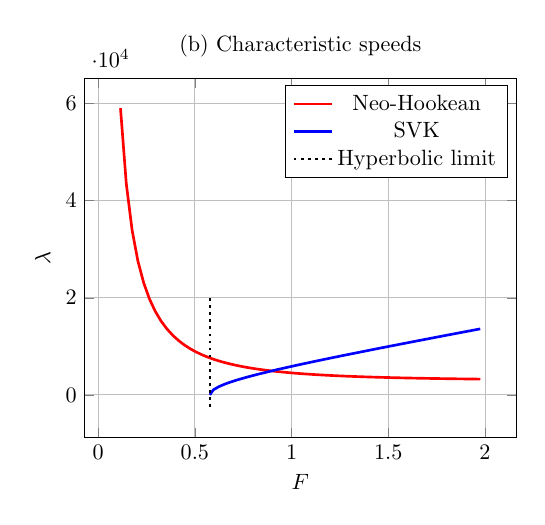
\begin{tikzpicture}[scale=0.8]
\begin{axis}[xlabel=$F$,ylabel=$\abs{\lambda}$,ymajorgrids=true,xmajorgrids=true,title={(b) Characteristic speeds}]
\addplot[Red,very thick] coordinates {(0.11547005383792518,59012.035730808406) (0.14547005383792516,43444.15680640866) (0.17547005383792513,33909.66271892359) (0.20547005383792513,27551.616086072518) (0.23547005383792513,23052.45426344622) (0.2654700538379251,19726.297080765253) (0.2954700538379251,17183.410876622853) (0.3254700538379251,15187.108927674422) (0.35547005383792507,13585.92851121213) (0.38547005383792504,12278.756336822797) (0.415470053837925,11195.691489974464) (0.44547005383792504,10286.970773511453) (0.475470053837925,9516.269220270638) (0.505470053837925,8856.492138358943) (0.535470053837925,8287.045413546242) (0.5654700538379249,7792.014425579814) (0.595470053837925,7358.918900548452) (0.625470053837925,6977.8428382999955) (0.6554700538379249,6640.81463208358) (0.6854700538379249,6341.3576871839605) (0.7154700538379248,6074.159484360366) (0.7454700538379249,5834.824367261866) (0.7754700538379249,5619.6864514897625) (0.8054700538379248,5425.666332338412) (0.8354700538379248,5250.16012367266) (0.8654700538379249,5090.952654625974) (0.8954700538379248,4946.148920983796) (0.9254700538379248,4814.119475233549) (0.9554700538379248,4693.456563660641) (0.9854700538379247,4582.938625301644) (1.0154700538379247,4481.501352586511) (1.0454700538379247,4388.21394243672) (1.0754700538379247,4302.259484218307) (1.1054700538379247,4222.918668359039) (1.1354700538379248,4149.556178447647) (1.1654700538379246,4081.609265724866) (1.1954700538379246,4018.57810915085) (1.2254700538379246,3960.0176447237714) (1.2554700538379246,3905.530610294456) (1.2854700538379247,3854.761601089376) (1.3154700538379245,3807.391969723345) (1.3454700538379245,3763.135435049281) (1.3754700538379245,3721.7342885593334) (1.4054700538379246,3682.9561065868374) (1.4354700538379246,3646.590892305437) (1.4654700538379246,3612.448584281259) (1.4954700538379244,3580.3568787248346) (1.5254700538379244,3550.1593210921387) (1.5554700538379245,3521.7136296737963) (1.5854700538379245,3494.8902195829423) (1.6154700538379245,3469.5709003379666) (1.6454700538379243,3445.6477242208375) (1.6754700538379244,3423.021965921998) (1.7054700538379244,3401.6032167766175) (1.7354700538379244,3381.308579249105) (1.7654700538379244,3362.061949309672) (1.7954700538379245,3343.793376030597) (1.8254700538379243,3326.438489161275) (1.8554700538379243,3309.9379866615427) (1.8854700538379243,3294.237175216221) (1.9154700538379243,3279.2855576483526) (1.9454700538379244,3265.0364619174256) (1.9754700538379242,3251.446707051308) };
\addplot[Blue,very thick] coordinates {(sqrt(1./3.),0.) (0.595470053837925,1048.9455179543422) (0.625470053837925,1731.1029259571128) (0.6554700538379249,2233.012146664284) (0.6854700538379249,2658.790029377158) (0.7154700538379248,3040.5889001561395) (0.7454700538379249,3393.286396027051) (0.7754700538379249,3725.1576526965905) (0.8054700538379248,4041.336632315833) (0.8354700538379248,4345.250197655363) (0.8654700538379249,4639.309436869055) (0.8954700538379248,4925.279696432755) (0.9254700538379248,5204.494537554574) (0.9554700538379248,5477.987035494905) (0.9854700538379247,5746.574266198714) (1.0154700538379247,6010.9138156437175) (1.0454700538379247,6271.542813975518) (1.0754700538379247,6528.905643538706) (1.1054700538379247,6783.374072186155) (1.1354700538379248,7035.262182069363) (1.1654700538379246,7284.837637447764) (1.1954700538379246,7532.330323596269) (1.2254700538379246,7777.939063134427) (1.2554700538379246,8021.836903239133) (1.2854700538379247,8264.175324905573) (1.3154700538379245,8505.087628335128) (1.3454700538379245,8744.691681060722) (1.3754700538379245,8983.092167747032) (1.4054700538379246,9220.382446402957) (1.4354700538379246,9456.646090866763) (1.4654700538379246,9691.958181097758) (1.4954700538379244,9926.386389147965) (1.5254700538379244,10159.991898394823) (1.5554700538379245,10392.830185782268) (1.5854700538379245,10624.951690800193) (1.6154700538379245,10856.402390269113) (1.6454700538379243,11087.224294354115) (1.6754700538379244,11317.455876364773) (1.7054700538379244,11547.132446624275) (1.7354700538379244,11776.286478876727) (1.7654700538379244,12004.947896244235) (1.7954700538379245,12233.144322567889) (1.8254700538379243,12460.901304010209) (1.8554700538379243,12688.242505014787) (1.8854700538379243,12915.189882077482) (1.9154700538379243,13141.763838254037) (1.9454700538379244,13367.983360890252) (1.9754700538379242,13593.866144695845) };
\addplot[dotted,very thick] coordinates {(sqrt(1./3.),-0.25e4) (sqrt(1./3.),2.e4)};
\legend{Neo-Hookean,SVK,Hyperbolic limit}
\end{axis}
\end{tikzpicture}
}
    \caption{Comparison of neo--Hookean and Saint-Venant--Kirchhoff hyperelastic models.}
    \label{fig:SVK-NH}
  \end{figure}
  At last, figure \ref{fig:SVK-NH}\subref{subfig:SVK_NH_Pi} highlights the non-physical behaviour of Saint-Venant-Kirchhoff model for high compression loads that lead to a stress tensor tending to zero.
\end{remark}


%%% Local Variables:
%%% mode: latex
%%% TeX-master: "../mainManuscript"
%%% End:


\section{Some solutions of Riemann problems}
\label{sec:riemann_problems}
The characteristic analysis carried out above is now applied to specific solid mechanics problems.
Both linear and non-linear problems, whose solutions involve several types of waves, are considered.
As we shall see, the different characteristic structures involved within linear elastic, elastoplastic and hyperelastic solids require the use of different techniques in order to develop exact solutions. First a particular type of IVP, of particular interest in this manuscript, is introduced.
%% Then by specializing the results to problems involving a linear elastic bar and a hyperelastic Saint-Venant-Kirchhoff medium, we shall see that different types of waves may propagate within solids.
\subsection{The Riemann problem}
A Riemann problem is a Cauchy problem with piecewise constant initial data. In particular, the Riemann problem based on the conservative form \eqref{eq:general_conservative_HE} for hyperelastic solids, in the arbitrary direction $\vect{N}=N_\alpha \vect{E}_\alpha$, takes the form:
\begin{equation}
  \label{eq:Riemann_problem_HE}
  \begin{aligned}
    &\Ucb_t + \drond{\Fcb\cdot \vect{N}}{X_N} = \Scb, \\
    &\left\lbrace 
      \begin{aligned}
        & \Ucb(X_N,t=0) = \Ucb^L \quad \text{if } X_N< 0\\
        & \Ucb(X_N,t=0) = \Ucb^R \quad \text{if } X_N> 0
      \end{aligned}
    \right.
  \end{aligned}
\end{equation}
Analogously, for small strains one writes the Riemann problem corresponding to conservative forms \eqref{eq:general_conservative} or \eqref{eq:general_conservative_EP} in the direction $\vect{n}=n_i \vect{e}_i$:
\begin{equation}
  \label{eq:Riemann_problem_HPP}
  \begin{aligned}
    &\Qcb_t + \drond{\Fcb\cdot \vect{n}}{x_n} = \Scb, \\
    &\left\lbrace 
      \begin{aligned}
        & \Qcb(x_n,t=0) = \Qcb^L \quad \text{if } x_n< 0\\
        & \Qcb(x_n,t=0) = \Qcb^R \quad \text{if } x_n> 0
      \end{aligned}
    \right.
  \end{aligned}
\end{equation}
where $x_n=\vect{x}\cdot\vect{n}$.
Problems of the form \eqref{eq:Riemann_problem_HE} or \eqref{eq:Riemann_problem_HPP} are considered in the next section, in which exact solutions are recalled or derived.

\subsection{Linear elastodynamics problems}
\label{subsec:charac_Linear_problems}
A homogeneous hyperbolic system of dimension $m$ is considered in a linear elastic solid so that a Riemann problem of the form \eqref{eq:Riemann_problem_HPP} is written.% in the arbitrary direction $\vect{n}$ reads:
% \begin{equation}
%   \label{eq:Linear_Riemann_problem}
%   \begin{aligned}
%   &\Qcb_t + \drond{\Fcb\cdot \vect{n}}{x_n} = \vect{0}, \\
%   &\left\lbrace 
%     \begin{aligned}
%       & \Qcb(x_n,t=0) = \Qcb^L \quad \text{if } x_n< 0\\
%       & \Qcb(x_n,t=0) = \Qcb^R \quad \text{if } x_n> 0
%     \end{aligned}
%     \right.
%   \end{aligned}
% \end{equation}

\subsubsection*{Characteristic variables -- Waves solution}
By introducing a set of \textit{characteristic variables} $\Pcb=\Rbsf^{-1}\Qcb$ ($\Rsf_{ij}=\Rc^j_i$), the quasi-linear form of system \eqref{eq:Riemann_problem_HPP} reads:
\begin{equation}
  \label{eq:RP_characteristic_variables}
  \begin{aligned}
    &\drond{\Pc_i}{t} + c_i\drond{\Pc_i}{x} = 0 \\
    &\left\lbrace 
      \begin{aligned}
        & \Pc_i(x,t=0) = \Pc_i^L \quad \text{if } x< 0\\
        & \Pc_i(x,t=0) = \Pc_i^R \quad \text{if } x> 0
      \end{aligned}
    \right.
  \end{aligned}
\end{equation}
with $\Csf_{ij}=c_i\delta_{ij}$, the matrix of eigenvalues so that $\Jsf_{ij} \Rc^j_K = \Rc^K_i\Csf_{Kj}$. The solution of this problem is straightforward since it corresponds to a superposition of scalar linear advection equations, namely, the initial profile $\Pc_i(x,t=0)$ simply propagates with speed $c_i$ as depicted in figure \ref{fig:advection}.  
\begin{figure}[h!]
  \centering
  \subcaptionbox*{}[0.45\linewidth]{\begin{tikzpicture}[scale=0.75]
  \draw[->] (-4,0) -- (4.,0) node[right] {$x$};
  \draw[->] (0,0) -- (0,4.5) node[above] {$t$};
  \draw[thick] (0,0) -- (4.,4) node [right] {$c_i$};
  % \fill[black] (1.,3.) circle (0.05) node [above] {$P$};
  % \fill[black] (2.10,1.762499) circle (0.05) node [right] {$P'$};
  \draw[dotted] (-4,1.)-- (0,1) node [above left] {$t_1$} --(4.,1);
  \draw[dotted] (-4,2.)-- (0,2) node [above left] {$t_2$} --(4.,2);
  \node[above left] at (0,0) {$t_0$};
\end{tikzpicture}

%%% Local Variables:
%%% mode: latex
%%% TeX-master: "../../mainManuscript"
%%% End:}
  \subcaptionbox*{}[0.45\linewidth]{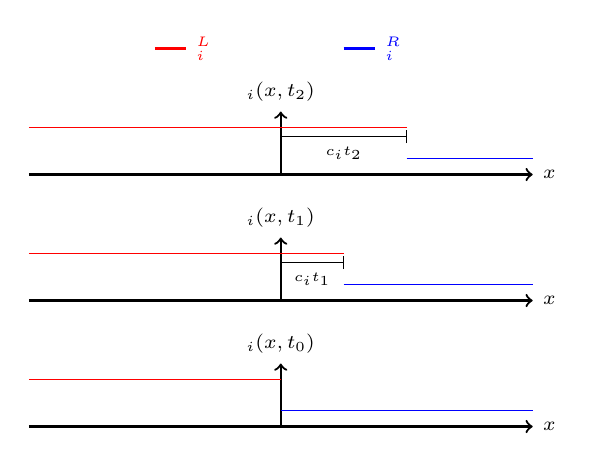
\begin{tikzpicture}[scale=0.8]
  %% t2
  \draw[->,thick] (0,0) -- (0,1) node [above] {\scriptsize$\Pc_i(x,t_2)$};
  \draw[->,thick] (-4,0) -- (4,0) node [right] {\scriptsize$x$};
  \draw[Blue] (2,0.25) -- (4,0.25);
  \draw[Red] (-4,0.75) -- (2,0.75);
  \draw (0,0.6)--(2,0.6) node [midway, below] {\tiny $c_it_2$};
  \draw (2,0.5)--(2,0.7);
  %% t1
  \draw[->,thick] (0,-2) -- (0,-1) node [above] {\scriptsize$\Pc_i(x,t_1)$};
  \draw[->,thick] (-4,-2) -- (4,-2) node [right] {\scriptsize$x$};
  \draw[Blue] (1,0.25-2) -- (4,0.25-2);
  \draw[Red] (-4,0.75-2) -- (1,0.75-2);
  \draw (0,0.6-2)--(1,0.6-2) node [midway, below] {\tiny $c_it_1$};
  \draw (1,0.5-2)--(1,0.7-2);
  %% t0
  \draw[->,thick] (0,-4) -- (0,-3) node [above] {\scriptsize$\Pc_i(x,t_0)$};
  \draw[->,thick] (-4,-4) -- (4,-4) node [right] {\scriptsize$x$};
  \draw[Blue] (0,0.25-4.) -- (4,0.25-4.);
  \draw[Red] (-4,0.75-4.) -- (0,0.75-4.);
  %% legend
  \draw[thick,Red] (-2.,2.) -- (-1.5,2.) node [right] {\scriptsize$\Pc_i^L$};
  \draw[thick,Blue] (1,2.) -- (1.5,2.) node [right] {\scriptsize$\Pc_i^R$};
\end{tikzpicture}
%%% Local Variables:
%%% mode: latex
%%% TeX-master: "../../mainManuscript"
%%% End:}
  \caption{Solution to linear advection equation of the quantity $\Pc_i$ with characteristic speed $c_i$.}
  \label{fig:advection}
\end{figure}
Thus, the solution  $\Pc_i(x,t)$ at a given point is given by tracing backward the characteristic of slope $c_i$ passing through this point to the $x$-axis, that is: $\Pc_i(x,t)=\Pc_i(x-c_it,0)$  \cite[p.52]{Toro}. The vector $\Qcb$ is then determined by inverting the relation:
\begin{equation}
  \label{eq:Q_expansion}
  \Qcb(x,t) = \sum_{i=1}^m \Rcb^i \Pc_i(x-c_it,0) \quad \Rightarrow
  \left\lbrace
    \begin{aligned}
      & \Qcb(x<0,0)=\Qcb^L=\sum_{i=1}^{m}\Rcb^i \Pc_i^L\\
      & \Qcb(x>0,0)=\Qcb^R= \sum_{i=1}^{m}\Rcb^i \Pc_i^R
    \end{aligned}
    \right.
\end{equation}
Equation \eqref{eq:Q_expansion} is an eigenvector expansion with coefficients $\Pc_i^{R,L}$ from which we see that $\Qcb$ is a linear superposition of $m$ waves, each having the shape $\Rcb^i \Pc_i(x,0)$.
Noticing that for given values of $x$ and $t$, there exists one characteristic $I$ such that $x-c_i t >0$ for all $i\leq I$, and $x-c_{i} t <0$ for all $i \geq I+1$, equation \eqref{eq:Q_expansion} can be rewritten \cite[p.56]{Toro}:
\begin{equation}
  \label{eq:Q_expansion_sides}
  \Qcb = \sum_{i=1}^I \Rcb^i \Pc_i^R + \sum_{i=I+1}^m \Rcb^i \Pc_i^L
\end{equation}
or, by introducing the expansions of initial data \eqref{eq:Q_expansion_sides}:
\begin{align}
  &\Qcb = \sum_{i=1}^m \Rcb^i \Pc_i^R - \sum_{i=I+1}^m \Rcb^i \(\Pc_i^R - \Pc_i^L\)= \Qcb^R - \sum_{i=I+1}^m \Rcb^i \(\Pc_i^R - \Pc_i^L\) \\
  &\Qcb= \sum_{i=1}^{m}\Rcb^i \Pc_i^L + \sum_{i=1}^I \Rcb^i \(\Pc_i^R - \Pc_i^L\)= \Qcb^L + \sum_{i=1}^I \Rcb^i \(\Pc_i^R - \Pc_i^L\) 
\end{align}
These equations are equivalent to jump conditions across multiple discontinuous waves:
\begin{align}
  \label{eq:jump_star_R}
  &  \Qcb-\Qcb^R = -\sum_{i=I+1}^{m} \Rcb^i\delta^i \\
  \label{eq:jump_star_L}
  &  \Qcb-\Qcb^L = \sum_{i=1}^{I} \Rcb^i\delta^i 
\end{align}
where $\Qcb(x,t)$ is the state lying in the region of the ($x,t$) plane delimited by the characteristics $I$ and $I+1$, and $\Rcb^i\delta^i$ the jump carried by the $i$th wave.
The coefficients $\delta^i=\Pc_i^R - \Pc_i^L$ are weighting coefficients involved in \textit{wave strengths} $\Wcb^i=\Rcb^i \delta^i$, that can be computed from the expansions of initial conditions by solving:
\begin{equation}
  \label{eq:delta_system}
  \Qcb^R-\Qcb^L=\sum_{i=1}^{m}\Rcb^i \delta^i=\Rbsf \vect{\delta}
\end{equation}

We see that the solutions of Riemann problem  \eqref{eq:Riemann_problem_HPP} consist of discontinuous waves emanating from the origin of the $(x,t)$ plane.
Across such discontinuous waves, the following condition is satisfied \cite{Toro}:
\begin{definition}
  The \textbf{Rankine-Hugoniot condition} is satisfied across a discontinuous wave of speed $s_i$ associated with the $i$th characteristic field, which is a solution of the hyperbolic system $\Qcb_t + \Fcb(\Qcb)_x=\vect{0}$:
\begin{equation}
  \label{eq:rankine-hugoniot}
  \saut{ \Fcb} = s_i \saut{ \Qcb}
\end{equation}
where $\saut{\bullet}$ denotes the jump operator across the discontinuity.
More specifically, shock waves that will be met for non-linear problems in section \ref{sec:SVK_solution} also satisfy the Rankine-Hugoniot condition.
\end{definition}

\subsubsection*{Solution of the elastic bar problem}
The above discussion is now specified to a one-dimensional elastic medium, $x\in\[-l,l\]$, of density $\rho$ undergoing one-dimensional stress and strain states within the infinitesimal framework: $\tens{\eps}=\eps\: \vect{e}_1\otimes \vect{e}_1$ ; $\tens{\sigma}=\sigma \:\vect{e}_1\otimes \vect{e}_1$. As a consequence, the bar hypothesis holds with $\vect{v}=v \vect{e}_1$. Neglecting body forces and introducing \textit{Young's modulus E} such that $\sigma = E\eps$, the Riemann problem takes the form \eqref{eq:Riemann_problem_HPP} with conserved quantities and flux vector:
\begin{equation*}
  \Qcb = \matrice{v \\ \sigma} \quad ; \quad \Fcb = \matrice{-\frac{1}{\rho}\sigma \\ -Ev}
\end{equation*}
along with Riemann-type data on the horizontal velocity (\textit{i.e. }$v(x<0,0)=v_L\:;\:v(x>0,0)=v_R$) as initial conditions. In addition, the solid is assumed to be initially unstressed. The eigenvalues, left and right eigenvectors of the corresponding Jacobian matrix are:
\begin{equation*}
  c=\pm\sqrt{\frac{E}{\rho} }  \quad ; \quad \Lcb^p=\[\rho c_p \:,\: -1\] \quad ; \quad \Rcb^p=\matrice{1\\- \rho c_p } 
\end{equation*}
The characteristic structure of the solution consisting of two elastic discontinuities emanating from the origin of the ($x,t$) plane is depicted in figure \ref{fig:elasticity_example}.
\begin{figure}[h]
  \centering
  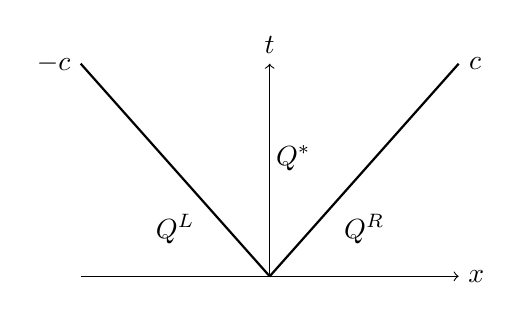
\begin{tikzpicture}[scale=0.6]
  \draw[->] (-4,0) -- (4.,0) node[right] {$x$};
  \draw[->] (0,0) -- (0,4.5) node[above] {$t$};
  \draw[thick] (0,0) -- (4.,4.5) node [right] {$c$};
  \draw[thick] (0,0) -- (-4.,4.5) node [left] {$-c$};
  \node at (2.,1.) {$\vect{Q}^R$};
  \node at (-2.,1.) {$\vect{Q}^L$};
  \node at (0.5,2.5) {$\vect{Q}^*$};
\end{tikzpicture}



%%% Local Variables:
%%% mode: latex
%%% TeX-master: "../../mainManuscript"
%%% End:

  \caption{Solution to Riemann problem  \eqref{eq:Riemann_problem_HPP} for an elastic bar.}
  \label{fig:elasticity_example}
\end{figure}
The solution $\Qcb^*$ lying in the region bounded by the two elastic waves is computed by means of equation \eqref{eq:jump_star_L} after solving \eqref{eq:delta_system} for the wave strength coefficients. For a system of dimension $2$ by writing $\Qcb^R-\Qcb^L=\Delta \Qcb$ those wave strengths read:
%For a system of dimension $2$, the solution in terms of wave strengths coefficients of system \eqref{eq:delta_system} is, by writing $\Qcb^R-\Qcb^L=\Delta \Qcb$:
%Writing $\Qcb^R-\Qcb^L=\Delta \Qcb$, linear systems of dimension $2$ lead to wave strengths coefficients:
\begin{equation}
  \label{eq:wave_strengths}
  \vect{\delta} = \frac{1}{\Rc^1_1\Rc^2_2 -\Rc_1^2\Rc^1_2}\matrice{\Rc^2_2\Delta \Qc_1 - \Rc^2_1\Delta \Qc_2 \\ \Rc^1_1\Delta \Qc_2 - \Rc_2^1\Delta \Qc_1}
\end{equation}
and more specifically for a bar:
\begin{equation}
  \label{eq:wave_strengths_bar}
  \vect{\delta} = \frac{1}{2\rho c}\matrice{\rho c \Delta v + \Delta \sigma \\  \rho c \Delta v -\Delta \sigma }
\end{equation}
Hence, equation \eqref{eq:jump_star_L} yields the solution:
\begin{equation}
  \label{eq:solution_charac_variables}
  \Qcb^* = \Qcb^L +\Rcb^1 \delta^1 = \matrice{\frac{\sigma_R - \sigma_L}{2\rho c} + \frac{v_R+v_L}{2} \\ \rho c\frac{v_R - v_L}{2} + \frac{\sigma_R+\sigma_L}{2}} 
\end{equation}


\subsection{Elastic-plastic media in the geometrical linearized limit}
\label{subsec:elasto-plastic_problem}
The previous problem is now extended to elastoplastic media by considering the same bar made of a linear hardening material of tensile yield stress $\sigma^y$. For such a solid domain, a Riemann problem of the form \eqref{eq:Riemann_problem_HPP} can be written by means of the following conserved quantities and flux vectors \cite{Thomas_EP}:
\begin{equation*}
  \Qcb = \matrice{v \\ \sigma} \quad ; \quad \Fcb = \matrice{-\frac{1}{\rho}\sigma \\ -Hv}
\end{equation*}
where $H=E$ for elastic loadings while $H=d\sigma/d\eps$ is the tangent modulus for elastic-plastic evolutions. In addition, Riemann-type data on the horizontal velocity (\textit{i.e. }$v(x<0,0)=v_L\:;\:v(x>0,0)=v_R$) are used as initial conditions, so that plastic flow may occur.

%We now generalize the previous discussion to elastoplastic solids within the small strains framework. A plane wave problem in an infinite elastoplastic medium with linear hardening is then considered. Such a plane wave can be due for instance to Riemann-type data on the horizontal velocity (\textit{i.e. }$v(x<0,0)=v_L\:;\:v(x>0,0)=v_R$) so that plastic flow may occur.
% The exact solution of such a linear problem being known \cite{Wang} an exact Riemann solver, which however requires a particular procedure, may be used.
The discontinuity of $H$ across the plastic threshold prevents here the direct derivation of the solution by using the approach followed for linear elasticity. Indeed, two sets of characteristic speeds and associated eigenvectors must be considered, that is \cite{Thomas_EP,Wang}:
\begin{equation*}
  c=\pm\sqrt{\frac{H}{\rho} } \quad ; \quad \Lcb^p=\[\rho c_p \:,\: -1\] \quad ; \quad \Rcb^p=\matrice{1\\- \rho c_p } 
\end{equation*}
so that waves are referred to as elastic or plastic waves. Whether a plastic wave appears or not hence depends on the tangent modulus and subsequently, on the yield function.
A predictor-corrector procedure must thus be followed by first solving an elastic Riemann problem whose resulting (trial) solution $\Qcb$ is tested against the yield criterion on both sides $x<0$ or $x>0$.
In general, possibly different yield stresses, plastic strains and hardening parameters in left and right regions lead to a yield criterion that may be violated or not, and hence to one, two or no plastic waves that must be added as a correction to the original problem.
If neither $f_L$ nor $f_R$ leads to a violation of the criterion, the problem is elastic and the trial state is the solution.
Otherwise, the plastic correction is performed by computing the stress in regions of the ($x,t$) plane bounded by elastic and plastic waves ($\tilde{\Qcb}^{L,R}$ in figure \ref{fig:EP_bar_solution}\subref{subfig:ep_bar_charac_4waves}) so that the yield function satisfies $f_{L,R}=0$.
\begin{figure}[h!]
  \centering
  \subcaptionbox{Characteristic structure\label{subfig:ep_bar_charac_4waves}}{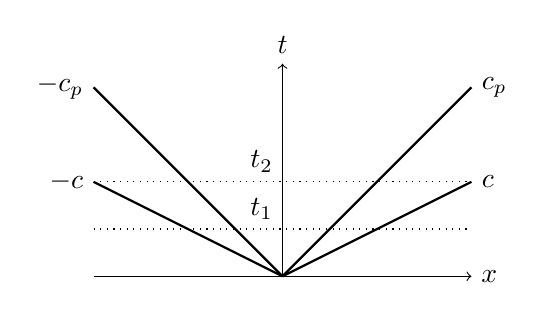
\begin{tikzpicture}[scale=0.6]
  \draw[->] (-4,0) -- (4.,0) node[right] {$x$};
  \draw[->] (0,0) -- (0,4.5) node[above] {$t$};
  \draw[thick] (0,0) -- (4.,2) node [right] {$c$};
  \draw[thick] (0,0) -- (4.,4) node [right] {$c_p$};
  \draw[thick] (0,0) -- (-4.,2) node [left] {$-c$};
  \draw[thick] (0,0) -- (-4.,4) node [left] {$-c_p$};
  \draw[dotted] (-4,1.)-- (0,1) node [above left] {$t_1$} --(4.,1);
  \draw[dotted] (-4,2.)-- (0,2) node [above left] {$t_2$} --(4.,2);
\end{tikzpicture}

%%% Local Variables:
%%% mode: latex
%%% TeX-master: "../../mainManuscript"
%%% End:}
  \subcaptionbox{Stress profile in the bar\label{subfig:ep_bar_stress_4waves}}{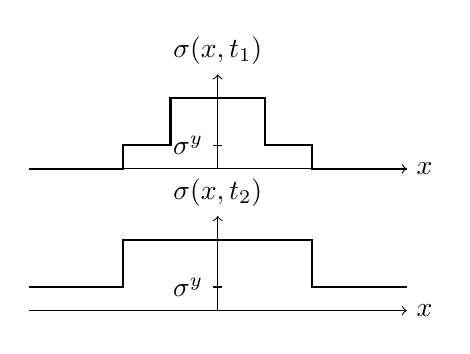
\begin{tikzpicture}[scale=0.6]
\draw[->] (0,0) -- (0,2) node [above] {$\sigma(x,t_1)$};
\draw[->] (-4,0) -- (4,0) node [right] {$x$};
\draw[thick] (-4,0) --(-2,0) -- (-2,0.5) -- (-1,0.5) -- (-1,1.5) -- (1,1.5) -- (1,0.5) -- (2,0.5) -- (2,0) -- (4,.0);
\draw (-0.1,0.5) node[left] {$\sigma^y$}-- (0.1,0.5);

\draw[->] (0,0-3) -- (0,2-3) node [above] {$\sigma(x,t_2)$};
\draw[->] (-4,0-3) -- (4,0-3) node [right] {$x$};
\draw[thick] (-4,0.5-3)  -- (-2,0.5-3)  --(-2,1.5-3) -- (2,1.5-3) -- (2,.5-3) -- (4,.5-3);
\draw (-0.1,0.5-3) node[left] {$\sigma^y$}-- (0.1,0.5-3);

\end{tikzpicture}}
  % \\\subcaptionbox{3-waves solution ($\sigma_L^y>\sigma_R^y$)\label{subfig:ep_bar_charac_3waves}}{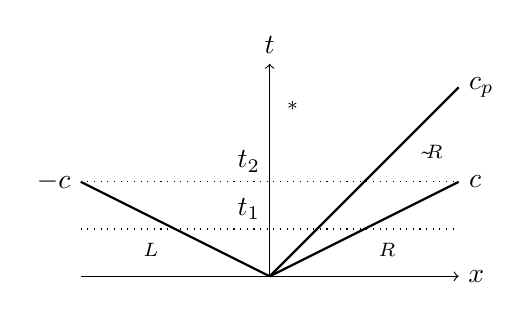
\begin{tikzpicture}[scale=0.6]
  \draw[->] (-4,0) -- (4.,0) node[right] {$x$};
  \draw[->] (0,0) -- (0,4.5) node[above] {$t$};
  \draw[thick] (0,0) -- (4.,2) node [right] {$c$};
  \draw[thick] (0,0) -- (4.,4) node [right] {$c_p$};
  \draw[thick] (0,0) -- (-4.,2) node [left] {$-c$};
  %\draw[thick] (0,0) -- (-4.,4) node [left] {$-c_p$};
  \draw[dotted] (-4,1.)-- (0,1) node [above left] {$t_1$} --(4.,1);
  \draw[dotted] (-4,2.)-- (0,2) node [above left] {$t_2$} --(4.,2);
  \node at (-2.5,0.) [above]{$\Qcb^L$};
  \node at (+2.5,0.) [above] {$\Qcb^R$};
  %\node at (-3.5,2.5) {$\tilde{\Qcb}^L$};
  \node at (+3.5,2.5) {$\tilde{\Qcb}^R$};
  \node at (0.5,3.5)  {$\Qcb^*$};
\end{tikzpicture}

%%% Local Variables:
%%% mode: latex
%%% TeX-master: "../../mainManuscript"
%%% End:}
  % \subcaptionbox{Stress for 3-waves($\sigma_L^y>\sigma_R^y$)\label{subfig:ep_bar_stress_3waves}}{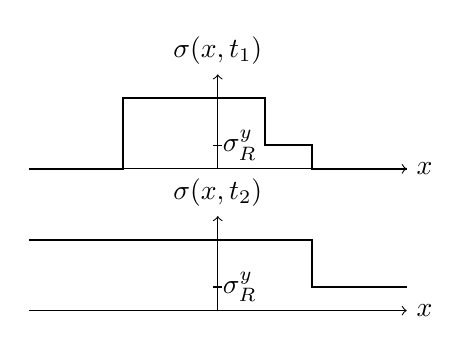
\begin{tikzpicture}[scale=0.6]
\draw[->] (0,0) -- (0,2) node [above] {$\sigma(x,t_1)$};
\draw[->] (-4,0) -- (4,0) node [right] {$x$};
\draw[thick] (-4,0) --(-2,0) -- (-2,1.5) -- (-0,1.5) -- (-0,1.5) -- (1,1.5) -- (1,0.5) -- (2,0.5) -- (2,0) -- (4,.0);
\draw (-0.1,0.5) node[right] {$\sigma_R^y$}-- (0.1,0.5);

\draw[->] (0,0-3) -- (0,2-3) node [above] {$\sigma(x,t_2)$};
\draw[->] (-4,0-3) -- (4,0-3) node [right] {$x$};
\draw[thick] (-4,1.5-3)  -- (-0,1.5-3)  --(-0,1.5-3) -- (2,1.5-3) -- (2,.5-3) -- (4,.5-3);
\draw (-0.1,0.5-3) node[right] {$\sigma_R^y$}-- (0.1,0.5-3);

\end{tikzpicture}}
  \caption{Example of a solution of a Riemann problem in a homogeneous elastoplastic bar with linear hardening and initial plastic strain $\eps^p(x,0)= 0$.}
  \label{fig:EP_bar_solution}
\end{figure}
Then, the velocity and elastic wave strengths in yielding regions are given by solving:
\begin{align}
  & \tilde{\Qcb}^R = \Qcb^R - \delta^1_E \Rcb^1_E\\
  & \tilde{\Qcb}^L = \Qcb^L + \delta^2_E \Rcb^2_E
\end{align}
At last a plastic Riemann solver is used in order to compute the solution of the problem $\Qcb^*$ by solving successively the system \eqref{eq:delta_system} for plastic wave strengths, and either system \eqref{eq:jump_star_R} or \eqref{eq:jump_star_L}, that is:
\begin{equation}
  \label{eq:plastic_approx_RS}
  \vect{\delta}_P = \Rbsf^{-1}\(\tilde{\Qcb}^R- \tilde{\Qcb}^L\) \quad \Rightarrow \quad
  \Qcb^* = \left\lbrace
  \begin{aligned}
      &  \tilde{\Qcb}^R - \delta_P^2 \Rcb^2_P\\
      &  \tilde{\Qcb}^L + \delta_P^1 \Rcb^1_P
  \end{aligned}
  \right.
\end{equation}

 Figure \ref{fig:EP_bar_solution}\subref{subfig:ep_bar_charac_4waves} shows the characteristic structure of the solution of the Riemann problem in a homogeneous medium considered here, involving two plastic waves, and figure \ref{fig:EP_bar_solution}\subref{subfig:ep_bar_stress_4waves} the corresponding stress field in the bar.

\begin{remark}
  Note that the above solver also applies to plane wave problems characterized by one-dimensional strain and multi-dimensional stress states by considering different wave speeds.
\end{remark}


\subsection{Hyperelastic media: A Saint-Venant-Kirchhoff solution}
\label{sec:SVK_solution}
The approaches followed above are no longer possible for problems involving a non-linear Jacobian matrix. Indeed, the writing of the Riemann problem \eqref{eq:RP_characteristic_variables} in terms of characteristic variables is valid for right eigenvectors that are constant. 
%since right eigenvectors cannot be taken out of the derivatives.
Moreover, as we shall see with an example, the characteristic structure of such problems can be more complex and depend on the initial data. 
%%% Picard problem
Consider a hyperelastic medium made of a Saint-Venant-Kirchhoff material, infinite in directions $\vect{E}_2$ and $\vect{E}_3$, and semi-infinite in direction $\vect{E}_1$ (\textit{i.e. $X_1 \in [0,+\infty[$}) in the reference configuration. This medium suddenly undergoes a load at $(X_1=X=0,t=0)$ in direction $\vect{E}_1$ so that the deformation gradient and the PK1 tensors are respectively of the form:
\begin{align}
  \label{eq:SVK_plane_wave}
  &\tens{F}=F\vect{e}_1\otimes\vect{E}_1 + \vect{e}_2\otimes\vect{E}_2 + \vect{e}_3\otimes\vect{E}_3 \\
  & \tens{\Pi}=\Pi_{11}\vect{e}_1\otimes\vect{E}_1 + \Pi_{22}\(\vect{e}_2\otimes\vect{E}_2 + \vect{e}_3\otimes\vect{E}_3 \)
\end{align}
which corresponds to a plane wave solution. We assume that $F(0,t)=\bar{F}$ is given, leading to a \textit{Picard problem} \cite[p.20]{Wang} involving both initial and boundary conditions with neglected body forces:
\begin{equation}
  \label{eq:Picard_problem}
  \begin{aligned}
  &\Qcb_t + \drond{\Fcb\cdot \vect{N}}{X_N} = \vect{0}, \\
  &\left\lbrace 
    \begin{aligned}
      & \Qcb(X_N,t=0) = \Qcb^R \quad \text{if } X_N> 0 \\
      & F(0,t) = \bar{F} 
    \end{aligned}
    \right.
  \end{aligned}
\end{equation}
with $\vect{N}=\vect{E}_1$ and:
\begin{equation*}
 \Qcb = \matrice{v \\ F} \quad ; \quad \Fcb = \matrice{-\frac{1}{\rho_0}\Pi \\ -v}
\end{equation*}
where $\Pi=\Pi_{11}$.
%%%
%Since the tangent modulus and the acoustic tensor of Saint-Venant-Kirchhoff model \eqref{eq:SVK_tangent},\eqref{eq:SVK_acoustic} depend on the deformation gradient, the quasi-linear form: $\Qcb_t + \drond{\Fcb}{\Qcb}\drond{\Qcb}{X}=\vect{0}$ is more convenient. The Jacobian matrix is then:
The quasi-linear form is written by using the chain rule: $\Qcb_t + \drond{\Fcb}{\Qcb}\drond{\Qcb}{X}=\vect{0}$ so that the Jacobian matrix reads:
\begin{equation}
  \label{eq:quasi_SVK}
  \Jbsf=\drond{\Fcb}{\Qcb}=-\matrice{0 & \frac{H_{1111}}{\rho_0} \\ 1 & 0}
\end{equation}
The tangent modulus of the SVK model \eqref{eq:SVK_tangent} yields the following characteristic fields:
\begin{equation}
  \label{eq:SVK_charac_fields}
  \left\lbrace
    \begin{aligned}
      & c_1=- \sqrt{\frac{\lambda+2\mu}{2\rho_0}\(3F^2-1\) }\\
      &c_2= \sqrt{\frac{\lambda+2\mu}{2\rho_0}\(3F^2-1\) }
    \end{aligned}\right.
 \quad ; \quad \Lcb^p=\[1\:,\:- c_p \] \quad ; \quad \Rcb^p=\matrice{- c_p \\1} 
\end{equation}

\begin{remark}
  \label{rq:hyperbolicity_limit_SVK}
  The non-linear flux function of the SVK model yields characteristic fields depending on the strain state and possibly complex celerities leading to a loss of hyperbolicity of the problem for $F<\sqrt{\frac{1}{3}}$.
\end{remark}

Suppose now that initial data are given so that $\bar{F} > F_R$. The resulting characteristic speeds then satisfy $c_2(\bar{F})>c_2(F_R)$ and the two families of characteristics collide in the right region of the ($x,t$) plane (figure \ref{fig:Picard_problem}\subref{subfig:2S}). On the other hand, $\bar{F} < F_R$ yields characteristics moving away from each other in the right region according to $c_2(\bar{F})<c_2(F_R)$ (figure \ref{fig:Picard_problem}\subref{subfig:2R}). These two situations respectively correspond to a shock and a simple wave. Note that this characteristic structure is similar to that resulting from the \textit{dam-break problem} with \textit{shallow water} equations, the following developments are hence very close to those of \cite[Ch.13]{Leveque}.
\begin{figure}[h!]
  \centering
  \subcaptionbox{Right-going shock wave\label{subfig:2S}}{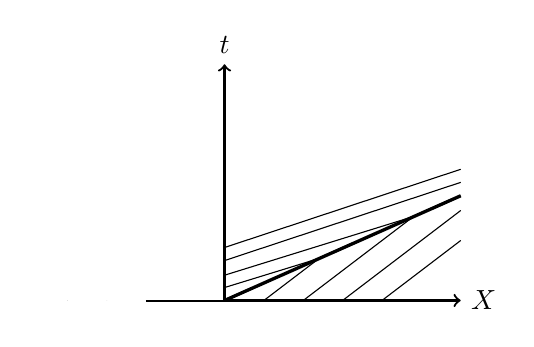
\begin{tikzpicture}
  \draw[->,thick] (-1,0) -- (3,0) node[right] {$X$};
  \draw[->,thick](0,0) -- (0,3) node[above] {$t$};
  \draw(-0.5,0.01) -- (1.20,0.533333) ;
  \draw(-1,0.01) -- (2.40,1.066) ;
  \draw(-1.5,0.01) -- (3,1.5) ;
  \draw(-2,0.01) -- (3,1.666) ;
  %%%%%%%%% 
  \draw(0.5,0) -- (1.20,0.533333) ;
  \draw(1.,0) -- (2.40,1.066) ;
  \draw(1.5,0) -- (3,1.14285) ;
  \draw(2.0,0) -- (3,0.7619) ;
  \draw[very thick] (0,0) -- (3,1.33);
  \fill[white] (-2.5,2.5) rectangle (-0.015,0.01);
  \fill[white] (-2.,0) rectangle (-1.,0.1);
\end{tikzpicture}}
  \subcaptionbox{Right-going simple wave\label{subfig:2R}}{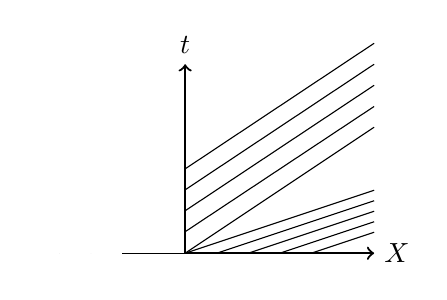
\begin{tikzpicture}[scale=0.8]
  \draw[->,thick] (-1,0) -- (3,0) node[right] {$X$};
  \draw[->,thick](0,0) -- (0,3) node[above] {$t$};
  \draw(0,0) -- (3,2) ;
  \draw(-0.5,0.01) -- (3,2.33) ;
  \draw(-1,0.01) -- (3,2.666) ;
  \draw(-1.5,0.01) -- (3,3) ;
  \draw(-2,0.01) -- (3,3.333) ;
  \draw(0,0) -- (3,1) ;
  \draw(0.5,0) -- (3,0.833) ;
  \draw(1,0) -- (3,0.666) ;
  \draw(1.5,0) -- (3,0.5) ;
  \draw(2,0) -- (3,0.333);
  \fill[white] (-2.5,2.5) rectangle (-0.015,0.01);
  \fill[white] (-2.,0) rectangle (-1.,0.1);
\end{tikzpicture}}
 \caption{Solutions of the Picard problem \eqref{eq:Picard_problem} depending on initial and boundary data.}
  \label{fig:Picard_problem}
\end{figure}

\subsubsection*{Shock waves}
% Applying the method of characteristics between the $x$-axis and an intersection point of two characteristic straight lines, one shows that a shock wave carry a jump discontinuity.
A shock wave is a discontinuous wave satisfying the Rankine-Hugoniot condition \eqref{eq:rankine-hugoniot}:
\begin{align}
  \label{eq:RH_velocity}
  & -\frac{1}{\rho_0}\(\bar{\Pi} - \Pi_i \) = s \( \bar{v} - v_i \)\\
  \label{eq:RH_F}
  & - \( \bar{v}-v_i\)=s\( \bar{F} - F_i\)
\end{align}
where the shock speed $s$ is to be defined and $i\in\{L,R\}$.
In what follows, $\bar{F}$ is considered as an unknown so that a relation connecting $\Qcb^i$ to a set of solutions $\Qcb$ through a shock wave can be developed.
Substitution of $s$ from equation \eqref{eq:RH_F} and introduction in equation \eqref{eq:RH_velocity} where $\Pi=\frac{\lambda+2\mu}{2}\(F^3-F\)$ yield:
\begin{align}
  \label{eq:shock_speed}
  & s=-\frac{\bar{v}-v_i}{\bar{F} - F_i}\\
  \label{eq:v_jump}
  & \bar{v}-v_i= \pm \sqrt{\frac{\lambda+2\mu}{2\rho_0}(\bar{F}-F_i)\[ \bar{F}^3-\bar{F} - (F_i^3-F_i)\]}
\end{align}
In addition to the Rankine-Hugoniot condition, one has to consider the \textit{Lax entropy conditions}, stating that characteristic curves collide in a shock wave \cite[p.268]{Leveque}:
\begin{equation}
  \label{eq:Lax_entropy}
  c(\bar{F})<s<c(F_i)
\end{equation}
The Lax entropy condition implies that the square root in equation \eqref{eq:v_jump} is real, leading to two families of curves in the phase plane ($F,v$). When considering an infinitesimal jump (\textit{i.e. $\bar{F}=F_i\pm\epsilon$ with $\epsilon \rightarrow 0$}), each of these curves is expected to identify with one of the jump conditions derived for the linear case \eqref{eq:jump_star_R} of \eqref{eq:jump_star_L}.
% One of those curve is expected to identify with the jump conditions derived for the linear case \eqref{eq:jump_star_R} when considering an infinitesimal jump (\textit{i.e. $\bar{F}=F_R+\epsilon$ with $\epsilon \rightarrow 0$}).
Thus, equation \eqref{eq:v_jump} reads:
\begin{equation}
  \label{eq:linearization}
  \bar{v}-v_i= \pm \sqrt{\frac{\lambda+2\mu}{2\rho_0}\epsilon\[ (F_i+\epsilon)^3-(F_i+\epsilon) - (F_i^3-F_i)\]}
\end{equation}
where, with $\epsilon \rightarrow 0$:
\begin{equation*}
  (F_i+\epsilon)^3\approx F_i^3(1+\frac{3\epsilon}{F_i})
\end{equation*}
so that:
\begin{equation*}
  \matrice{\bar{v} \\ \bar{F}}=\matrice{v_i \\ F_i} + \epsilon \matrice{\pm \sqrt{\frac{\lambda+2\mu}{2\rho_0}\[ 3F_i^2-1\]}\\1}
\end{equation*}
The minus sign yields equation \eqref{eq:jump_star_R} associated with the right-going wave and therefore corresponds to a right-going shock wave.
On the other hand, the plus sign stands for equation \eqref{eq:jump_star_L} and left-going shocks.
Finally, the Rankine-Hugoniot condition across a left-going shock and a right-going shock respectively lead to:
\begin{align}
  \label{eq:left-going_shock}
  &\bar{v}-v_L= \sqrt{\frac{\lambda+2\mu}{2\rho_0}(\bar{F}-F_L)\[ \bar{F}^3-\bar{F} - (F_L^3-F_L)\]} \\
  \label{eq:right-going_shock}
  &\bar{v}-v_R= -\sqrt{\frac{\lambda+2\mu}{2\rho_0}(\bar{F}-F_R)\[ \bar{F}^3-\bar{F} - (F_R^3-F_R)\]}
\end{align}

\subsubsection*{Simple waves}
In order to study the evolution of fields within the region bounded by characteristics that move away in figure \ref{fig:Picard_problem}\subref{subfig:2R}, let's write the left-going characteristic equation through it with $\Lcb^1=[1,-c_1]$:
\begin{equation}
  \label{eq:SVK_rarefaction}
  dv -c_1(F)  dF = 0 
\end{equation}
The complete set of states $\Qcb$ connected to $\Qcb^R$ through a simple wave is obtained by integration of equation \eqref{eq:SVK_rarefaction}. Note that this integration results in a smooth evolution of fields inside a simple wave even for discontinuous initial conditions, unlike shocks. Moreover, the vanishing right-hand side of the conservative form of the Picard problem \eqref{eq:Picard_problem} yields a similarity solution. The particular case of a simple wave constant along each ray $\xi=x/t$ corresponds to a \textit{rarefaction wave} \cite{Leveque}. 

Integration of equation \eqref{eq:SVK_rarefaction} is performed by using the change of variables: $F \mapsto ch(x)/\sqrt{3}$ so that one gets:
%The following change of variable is then introduced: $F \mapsto ch(x)/\sqrt{3}$, so that  becomes:
\begin{equation}
  \label{eq:charac_equation_sh}
  dv=-\sqrt{\frac{\lambda + 2\mu}{6\rho_0}}sh(x)^2 dx
\end{equation}
where, the hyperbolic cosine $ch(x)$ and sine $sh(x)$ satisfy: $ch(x)^2-sh(x)^2=1$. Equation \eqref{eq:charac_equation_sh} can be easily integrated with the exponential form of hyperbolic sine: $sh(x)=\frac{e^x - e^{-x}}{2}$, thus yielding:
\begin{equation*}
  v-v_R=-\frac{1}{4}\sqrt{\frac{\lambda + 2\mu}{6\rho_0}}\[sh(2x)-2x -(sh(2x_R)-2x_R)\]
\end{equation*}
At last, the inverse change of variables leads to the relation:
\begin{equation}
  \label{eq:integral_curve_right}
  v-v_R=-\sqrt{\frac{\lambda + 2\mu}{24\rho_0}}\[\sqrt{3}\(F\sqrt{3F^2-1} -F_R\sqrt{3F_R^2-1}\)-\ln\(\frac{\sqrt{3}F + \sqrt{3F^2-1}}{\sqrt{3}F_R + \sqrt{3F_R^2-1}}\) \]
\end{equation}
In a similar manner, $dv -c_2(F)  dF = 0$ must hold through a left-going rarefaction wave so that:
\begin{equation}
  \label{eq:integral_curve_left}
  v-v_L=\sqrt{\frac{\lambda + 2\mu}{24\rho_0}}\[\sqrt{3}\(F\sqrt{3F^2-1} -F_L\sqrt{3F_L^2-1}\)-\ln\(\frac{\sqrt{3}F + \sqrt{3F^2-1}}{\sqrt{3}F_L + \sqrt{3F_L^2-1}}\) \]
\end{equation}

Equations \eqref{eq:integral_curve_right} and \eqref{eq:integral_curve_left} correspond to \textit{integral curves} that connect initial conditions to a set of solutions through a right-going or a left-going rarefaction respectively.

\subsubsection*{Solution of the Riemann problem}
The above developments are now generalized by considering the Riemann problem in an infinite medium:
\begin{equation}
  \label{eq:HE_Riemann_problem}
  \begin{aligned}
    &\Qcb_t + \drond{\Fcb\cdot \vect{N}}{X_N} = \vect{0}, \\
    &\left\lbrace 
      \begin{aligned}
        & \Qcb(X_N,t=0) = \Qcb^L = \matrice{v=0 \\ F_L} \quad \text{if } X_N< 0\\
        & \Qcb(X_N,t=0) = \Qcb^R = \matrice{v=0 \\ F_R}\quad \text{if } X_N> 0
      \end{aligned}
    \right.
  \end{aligned}
\end{equation}
such that the plane wave state \eqref{eq:SVK_plane_wave} holds.
As for the Picard problem, initial conditions influence the characteristic structure of the solution. Indeed, if initial conditions are given such that $F_L<F_R$, left-going characteristics will collide while right-going ones will move away from one another (see figure \ref{fig:RP_solution}\subref{subfig:1S2R}). In that case, the first and second characteristic fields are respectively referred to as a \textit{1-shock} and a \textit{2-rarefaction}. Conversely, if $F_L>F_R$ the solution corresponds to a \textit{1-rarefaction} and a \textit{2-shock} (figure \ref{fig:RP_solution}\subref{subfig:1R2S}). 

\begin{figure}[h]
  \centering
  \subcaptionbox{$F_L < F_R$\label{subfig:1S2R}}{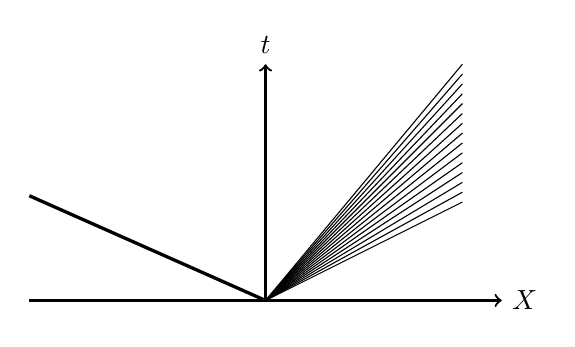
\begin{tikzpicture}
  \draw[->,thick] (-3,0) -- (3,0) node[right] {$X$};
  \draw[->,thick](0,0) -- (0,3) node[above] {$t$};
  %% Shock wave
  \draw[very thick] (0,0) -- (-3,1.33);
  %% Rarefaction wave
  \foreach \x in {0.5,0.55,...,1.25}
  \draw(0,0) -- (2.5,2.5*\x) ;
\end{tikzpicture}}
  \subcaptionbox{$F_L > F_R$\label{subfig:1R2S}}{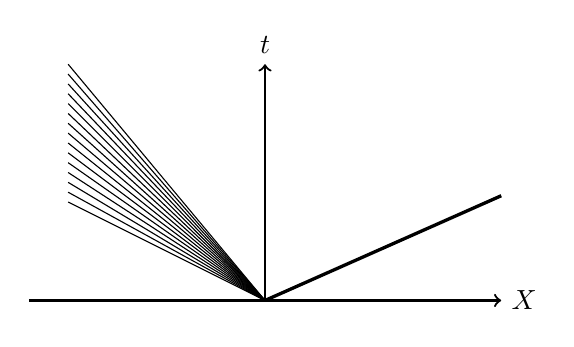
\begin{tikzpicture}
  \draw[->,thick] (-3,0) -- (3,0) node[right] {$X$};
  \draw[->,thick](0,0) -- (0,3) node[above] {$t$};
  %% Shock wave
  \draw[very thick] (0,0) -- (3,1.33);
  %% Rarefaction wave
  \foreach \x in {0.5,0.55,...,1.25}
  \draw(0,0) -- (-2.5,2.5*\x) ;
\end{tikzpicture}}
  \caption{General wave patterns arising in the solution of the Riemann problem \eqref{eq:HE_Riemann_problem} depending on initial data. (a): 1-shock--2-rarefaction. (b): 1-rarefaction--2-shock.}
  \label{fig:RP_solution}
\end{figure}

For the 1-shock--2-rarefaction solution one then seeks a state $\Qcb$ that is connected to $\Qcb^L$ and $\Qcb^R$ through a shock wave and a rarefaction wave respectively. Hence, $\Qcb$ must satisfy equations \eqref{eq:left-going_shock} and \eqref{eq:integral_curve_right}, that is:
\begin{equation}
  \label{eq:1S2R_solution}
  \left\lbrace
  \begin{aligned}
    &v -v_L= \sqrt{\frac{\lambda+2\mu}{2\rho_0}(F -F_L)\[ F^3-F  - (F_L^3-F_L)\]} \\
    &v -v_R=-\sqrt{\frac{\lambda + 2\mu}{24\rho_0}}\[\sqrt{3}\(F \sqrt{3F^2-1} -F_R\sqrt{3F_R^2-1}\)-\ln\(\frac{\sqrt{3}F  + \sqrt{3F^2-1}}{\sqrt{3}F_R + \sqrt{3F_R^2-1}}\) \]
  \end{aligned}
  \right.
\end{equation}
Analogously, the 1-rarefaction--2-shock solution is given by the solution of equations \eqref{eq:integral_curve_left} and \eqref{eq:right-going_shock}:
\begin{equation}
  \label{eq:1R2S_solution}
  \left\lbrace
  \begin{aligned}
    &v -v_L=\sqrt{\frac{\lambda + 2\mu}{24\rho_0}}\[\sqrt{3}\(F \sqrt{3F^2-1} -F_L\sqrt{3F_L^2-1}\)-\ln\(\frac{\sqrt{3}F  + \sqrt{3F^2-1}}{\sqrt{3}F_L + \sqrt{3F_L^2-1}}\) \]\\
    &v -v_R= -\sqrt{\frac{\lambda+2\mu}{2\rho_0}(F -F_R)\[ F^3-F  - (F_R^3-F_R)\]}
  \end{aligned}
  \right.
\end{equation}
\begin{figure}[h!]
  \centering
  {\definecolor{Purple}{RGB}{120,28,129}
\definecolor{Blue}{RGB}{63,96,174}
\definecolor{Duck}{RGB}{83,158,182}
\definecolor{Green}{RGB}{109,179,136}
\definecolor{Yellow}{RGB}{202,184,67}
\definecolor{Orange}{RGB}{231,133,50}
\definecolor{Red}{RGB}{217,33,32}
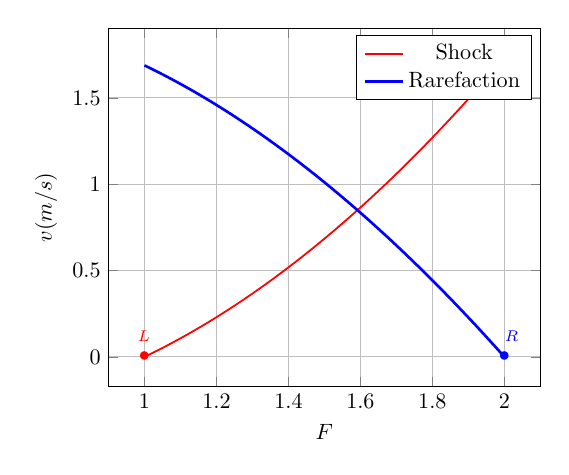
\begin{tikzpicture}[scale=0.8]
\begin{axis}[xlabel=$F$,ylabel=$v (m/s)$,ymajorgrids=true,xmajorgrids=true]
  \addplot[Red,thick] coordinates {(1.0,0.0) (1.0196019601960196,0.019889905868838792) (1.0392039203920391,0.04035480171519238) (1.058805880588059,0.06139339246981025) (1.0784078407840785,0.08300445472552491) (1.098009800980098,0.1051868317293367) (1.1176117611761176,0.1279394287977403) (1.1372137213721372,0.1512612091133456) (1.1568156815681567,0.17515118986560513) (1.1764176417641765,0.19960843870261852) (1.196019601960196,0.2246320704646163) (1.2156215621562156,0.25022124417291264) (1.2352235223522352,0.2763751602509047) (1.2548254825482548,0.30309305795616337) (1.2744274427442743,0.330374213004825) (1.2940294029402941,0.3582179353714115) (1.3136313631363137,0.386623567248899) (1.3332333233323332,0.4155904811553686) (1.3528352835283528,0.445118078174895) (1.3724372437243724,0.47520578632153143) (1.3920392039203922,0.5058530590163028) (1.4116411641164117,0.5370593736680643) (1.4312431243124313,0.568824230349938) (1.4508450845084508,0.6011471505637854) (1.4704470447044704,0.6340276760858663) (1.4900490049004902,0.667465367887438) (1.5096509650965095,0.7014598051246006) (1.5292529252925293,0.7360105841921958) (1.5488548854885489,0.7711173178369951) (1.5684568456845684,0.8067796343258441) (1.5880588058805882,0.8429971766647708) (1.6076607660766076,0.8797696018654025) (1.6272627262726274,0.917096580255355) (1.646864686468647,0.9549777948294852) (1.6664666466646665,0.9934129406392047) (1.686068606860686,1.032401724217221) (1.7056705670567056,1.0719438630353144) (1.7252725272527254,1.1120390849929296) (1.7448744874487447,1.1526871279345328) (1.7644764476447645,1.1938877391938512) (1.784078407840784,1.2356406751632294) (1.8036803680368036,1.2779457008865038) (1.8232823282328234,1.320802589673878) (1.8428842884288428,1.3642111227374165) (1.8624862486248626,1.4081710888458763) (1.8820882088208821,1.4526822839976499) (1.9016901690169017,1.4977445111107466) (1.9212921292129215,1.543357579728744) (1.9408940894089408,1.5895213057417645) (1.9604960496049606,1.6362355111215798) (1.9800980098009802,1.6835000236699957) (1.9996999699969997,1.7313146767797576) };
  \addplot[Blue,very thick] coordinates {(1.0,1.6884673989302577) (1.0196019601960196,1.6685781823289632) (1.0392039203920391,1.648117983645035) (1.058805880588059,1.6270917763366024) (1.0784078407840785,1.6055041425368688) (1.098009800980098,1.5833593157699348) (1.1176117611761176,1.5606612177002648) (1.1372137213721372,1.5374134899261505) (1.1568156815681567,1.5136195216278194) (1.1764176417641765,1.48928247372591) (1.196019601960196,1.4644053000848238) (1.2156215621562156,1.4389907661996928) (1.2352235223522352,1.4130414657294894) (1.2548254825482548,1.3865598351776642) (1.2744274427442743,1.3595481669723095) (1.2940294029402941,1.3320086211576845) (1.3136313631363137,1.3039432358761032) (1.3332333233323332,1.2753539367920979) (1.3528352835283528,1.246242545588463) (1.3724372437243724,1.216610787645106) (1.3920392039203922,1.1864602989961286) (1.4116411641164117,1.1557926326474621) (1.4312431243124313,1.12460926432638) (1.4508450845084508,1.092911597724879) (1.4704470447044704,1.0607009692909792) (1.4900490049004902,1.0279786526152188) (1.5096509650965095,0.994745862453826) (1.5292529252925293,0.9610037584250569) (1.5488548854885489,0.9267534484108921) (1.5684568456845684,0.8919959916925568) (1.5880588058805882,0.8567324018451127) (1.6076607660766076,0.8209636494135533) (1.6272627262726274,0.7846906643903794) (1.646864686468647,0.7479143385125069) (1.6664666466646665,0.7106355273934435) (1.686068606860686,0.6728550525050632) (1.7056705670567056,0.6345737030218022) (1.7252725272527254,0.595792237538853) (1.7448744874487447,0.5565113856747698) (1.7644764476447645,0.5167318495678894) (1.784078407840784,0.47645430527509447) (1.8036803680368036,0.43567940408061234) (1.8232823282328234,0.3944077737218566) (1.8428842884288428,0.3526400195386741) (1.8624862486248626,0.31037672555176576) (1.8820882088208821,0.2676184554755838) (1.9016901690169017,0.22436575367049583) (1.9212921292129215,0.18061914603862234) (1.9408940894089408,0.13637914086738703) (1.9604960496049606,0.09164622962443836) (1.9800980098009802,0.04642088770736517) (1.9996999699969997,0.0007035751512764867) };
  \node at (axis cs:1,0) [Red] {$\bullet$};
  \node at (axis cs:2.,0) [Blue] {$\bullet$};
  % \node[coordinate] at (axis cs:1.,0.) {$Mich$};
  \node at (axis cs:1,0) [anchor=south,Red] {$\Qcb^L$};
  \node at (axis cs:1.98,0) [above right,Blue] {$\Qcb^R$};
  \legend{Shock,Rarefaction}
  % \addplot[Blue,dashed,very thick,domain=1:2,samples=51,samples y=0]
  %   ({x},{0.-sqrt(0.5*(12.-1))*(x-2.)});
  % \addplot[Red,dashed,very thick,domain=1:2,samples=51,samples y=0]
  %   ({x},{0.+sqrt(0.5*(2.-1))*(x-1.)});
\end{axis}
\end{tikzpicture}
\phantomsubcaption \label{subfig:1S2R_curves}}
  {\definecolor{Purple}{RGB}{120,28,129}
\definecolor{Blue}{RGB}{63,96,174}
\definecolor{Duck}{RGB}{83,158,182}
\definecolor{Green}{RGB}{109,179,136}
\definecolor{Yellow}{RGB}{202,184,67}
\definecolor{Orange}{RGB}{231,133,50}
\definecolor{Red}{RGB}{217,33,32}
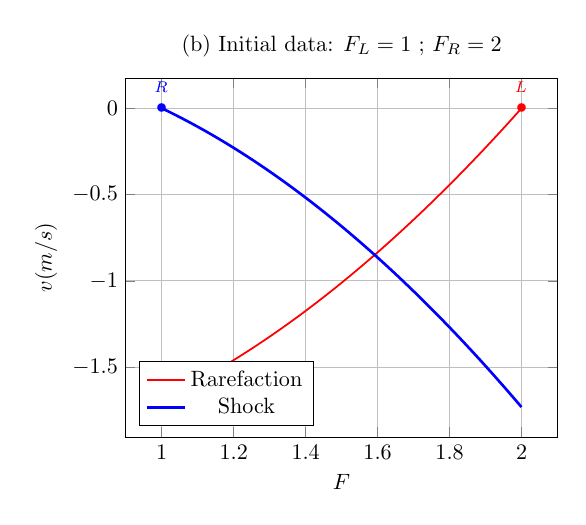
\begin{tikzpicture}[scale=0.8]
\begin{axis}[xlabel=$F$,ylabel=$v (m/s)$,ymajorgrids=true,xmajorgrids=true,legend pos=south west,title={(b) Initial data: $F_L=1$ ; $F_R=2$}]
  \addplot[Red,thick] coordinates {(1.0,-1.6884673989302577) (1.0196019601960196,-1.6685781823289632) (1.0392039203920391,-1.648117983645035) (1.058805880588059,-1.6270917763366024) (1.0784078407840785,-1.6055041425368688) (1.098009800980098,-1.5833593157699348) (1.1176117611761176,-1.5606612177002648) (1.1372137213721372,-1.5374134899261505) (1.1568156815681567,-1.5136195216278194) (1.1764176417641765,-1.48928247372591) (1.196019601960196,-1.4644053000848238) (1.2156215621562156,-1.4389907661996928) (1.2352235223522352,-1.4130414657294894) (1.2548254825482548,-1.3865598351776642) (1.2744274427442743,-1.3595481669723095) (1.2940294029402941,-1.3320086211576845) (1.3136313631363137,-1.3039432358761032) (1.3332333233323332,-1.2753539367920979) (1.3528352835283528,-1.246242545588463) (1.3724372437243724,-1.216610787645106) (1.3920392039203922,-1.1864602989961286) (1.4116411641164117,-1.1557926326474621) (1.4312431243124313,-1.12460926432638) (1.4508450845084508,-1.092911597724879) (1.4704470447044704,-1.0607009692909792) (1.4900490049004902,-1.0279786526152188) (1.5096509650965095,-0.994745862453826) (1.5292529252925293,-0.9610037584250569) (1.5488548854885489,-0.9267534484108921) (1.5684568456845684,-0.8919959916925568) (1.5880588058805882,-0.8567324018451127) (1.6076607660766076,-0.8209636494135533) (1.6272627262726274,-0.7846906643903794) (1.646864686468647,-0.7479143385125069) (1.6664666466646665,-0.7106355273934435) (1.686068606860686,-0.6728550525050632) (1.7056705670567056,-0.6345737030218022) (1.7252725272527254,-0.595792237538853) (1.7448744874487447,-0.5565113856747698) (1.7644764476447645,-0.5167318495678894) (1.784078407840784,-0.47645430527509447) (1.8036803680368036,-0.43567940408061234) (1.8232823282328234,-0.3944077737218566) (1.8428842884288428,-0.3526400195386741) (1.8624862486248626,-0.31037672555176576) (1.8820882088208821,-0.2676184554755838) (1.9016901690169017,-0.22436575367049583) (1.9212921292129215,-0.18061914603862234) (1.9408940894089408,-0.13637914086738703) (1.9604960496049606,-0.09164622962443836) (1.9800980098009802,-0.04642088770736517) (1.9996999699969997,-0.0007035751512764867) };
  \addplot[Blue,very thick] coordinates {(1.0,0.0) (1.0196019601960196,-0.019889905868838792) (1.0392039203920391,-0.04035480171519238) (1.058805880588059,-0.06139339246981025) (1.0784078407840785,-0.08300445472552491) (1.098009800980098,-0.1051868317293367) (1.1176117611761176,-0.1279394287977403) (1.1372137213721372,-0.1512612091133456) (1.1568156815681567,-0.17515118986560513) (1.1764176417641765,-0.19960843870261852) (1.196019601960196,-0.2246320704646163) (1.2156215621562156,-0.25022124417291264) (1.2352235223522352,-0.2763751602509047) (1.2548254825482548,-0.30309305795616337) (1.2744274427442743,-0.330374213004825) (1.2940294029402941,-0.3582179353714115) (1.3136313631363137,-0.386623567248899) (1.3332333233323332,-0.4155904811553686) (1.3528352835283528,-0.445118078174895) (1.3724372437243724,-0.47520578632153143) (1.3920392039203922,-0.5058530590163028) (1.4116411641164117,-0.5370593736680643) (1.4312431243124313,-0.568824230349938) (1.4508450845084508,-0.6011471505637854) (1.4704470447044704,-0.6340276760858663) (1.4900490049004902,-0.667465367887438) (1.5096509650965095,-0.7014598051246006) (1.5292529252925293,-0.7360105841921958) (1.5488548854885489,-0.7711173178369951) (1.5684568456845684,-0.8067796343258441) (1.5880588058805882,-0.8429971766647708) (1.6076607660766076,-0.8797696018654025) (1.6272627262726274,-0.917096580255355) (1.646864686468647,-0.9549777948294852) (1.6664666466646665,-0.9934129406392047) (1.686068606860686,-1.032401724217221) (1.7056705670567056,-1.0719438630353144) (1.7252725272527254,-1.1120390849929296) (1.7448744874487447,-1.1526871279345328) (1.7644764476447645,-1.1938877391938512) (1.784078407840784,-1.2356406751632294) (1.8036803680368036,-1.2779457008865038) (1.8232823282328234,-1.320802589673878) (1.8428842884288428,-1.3642111227374165) (1.8624862486248626,-1.4081710888458763) (1.8820882088208821,-1.4526822839976499) (1.9016901690169017,-1.4977445111107466) (1.9212921292129215,-1.543357579728744) (1.9408940894089408,-1.5895213057417645) (1.9604960496049606,-1.6362355111215798) (1.9800980098009802,-1.6835000236699957) (1.9996999699969997,-1.7313146767797576) };
  \node at (axis cs:1,0) [Blue] {$\bullet$};
  \node at (axis cs:2.,0) [Red] {$\bullet$};
  \node at (axis cs:1,0) [anchor=south,Blue] {$\Qcb^R$};
  \node at (axis cs:2,0) [anchor=south,Red] {$\Qcb^L$};
\legend{Rarefaction,Shock}
\end{axis}
\end{tikzpicture}
\phantomsubcaption  \label{subfig:1R2S_curves}}
  \caption{Set of connected states $\Qcb$ to initial data through shock and rarefaction waves with $v_L=v_R=0$ in both cases: (a) 1-shock, 2-rarefaction solution ; (b) 1-rarefaction, 2-shock.}
  \label{fig:solutions_RP}
\end{figure} 
Once one of these systems is solved, the solution $\Qcb$ is known everywhere except inside the rarefaction fan. Nevertheless, in this region $\Qcb$ only varies with the ray $\xi=c_i(F)$ and hence, the solution inside an $i$-rarefaction wave satisfies:
\begin{equation}
  \label{eq:rarefaction_fan}
  \xi = \pm \sqrt{\frac{\lambda + 2\mu}{2\rho_0}\(3F^2-1 \)} \quad \Rightarrow \quad F(\xi)= \sqrt{\frac{2\rho_0}{3(\lambda + 2\mu)}\xi^2-1}
\end{equation}

The curves corresponding to equations \eqref{eq:1S2R_solution} and \eqref{eq:1R2S_solution} are depicted in figures \ref{fig:solutions_RP}\subref{subfig:1S2R_curves} and \ref{fig:solutions_RP}\subref{subfig:1R2S_curves} for parameter values such that $\frac{\lambda+2\mu}{\rho_0}=1$. In both cases, the solution $\Qcb(x,t)$ in the region bounded by the shock and the rarefaction fan is given by the intersection of curves in the phase plane. 

\begin{remark}
  \label{rq:charach_neoHook}
  Note that the above developments are based on a constitutive model that leads to a concave flux function $\Fcb^T=-\[\frac{1}{\rho_0}\Pi \: ;\: v\]$ (\textit{i.e. } $\ddrond{\Pi}{F}{F}>0$). As a consequence, the characteristic speeds are monotonically increasing functions of the deformation gradient (in absolute value). Since the dependence of characteristic speeds on the deformation gradient governs the wave pattern (\textit{i.e.: either a rarefaction or a shock wave}), the structure of the solution differs from other constitutive laws with convex flux function such as the neo-Hookean model.
  Comparisons of ($F,\Pi_{11}$) and ($F,\abs{c}$) are shown in figures \ref{fig:SVK-NH}\subref{subfig:SVK_NH_Pi} and \ref{fig:SVK-NH}\subref{subfig:SVK_NH_speeds} as an illustration of previous remarks.
  \begin{figure}[h!]
    \centering
    {\definecolor{Red}{RGB}{217,33,32}
\definecolor{Blue}{RGB}{63,96,174}
\definecolor{Duck}{RGB}{83,158,182}
\definecolor{Green}{RGB}{109,179,136}
\definecolor{Yellow}{RGB}{202,184,67}
\definecolor{Orange}{RGB}{231,133,50}
\definecolor{Red}{RGB}{217,33,32}
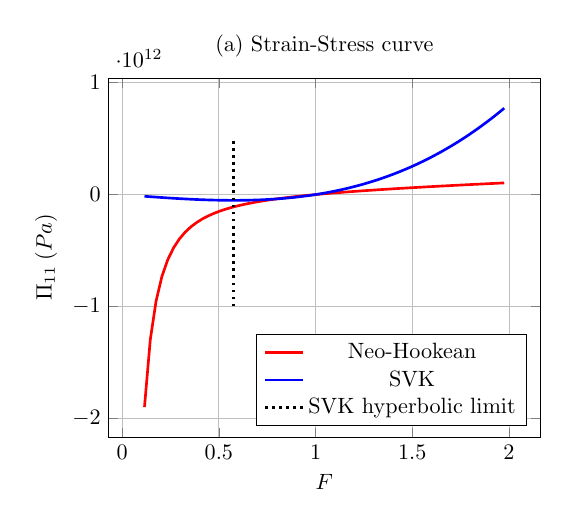
\begin{tikzpicture}[scale=0.8]
\begin{axis}[xlabel=$F$,ylabel=$\Pi_{11} \: (Pa)$,ymajorgrids=true,xmajorgrids=true,legend pos=south east,title={(a) Strain-Stress curve}]
\addplot[Red,very thick] coordinates {(0.11547005383792518,-1898966453319.162) (0.14547005383792516,-1296837707486.0405) (0.17547005383792513,-951312235719.5623) (0.20547005383792513,-732355105152.6451) (0.23547005383792513,-583575852118.2125) (0.2654700538379251,-477087968993.8754) (0.2954700538379251,-397729449724.4541) (0.3254700538379251,-336642141070.28204) (0.35547005383792507,-288349957545.72546) (0.38547005383792504,-249309520683.61847) (0.415470053837925,-217140040714.9308) (0.44547005383792504,-190190468824.5224) (0.475470053837925,-167284549773.97247) (0.505470053837925,-147564580724.34894) (0.535470053837925,-130392343185.27245) (0.5654700538379249,-115284401045.16144) (0.595470053837925,-101868733030.67676) (0.625470053837925,-89854990617.66492) (0.6554700538379249,-79013679521.07468) (0.6854700538379249,-69161318053.14328) (0.7154700538379248,-60149680216.69014) (0.7454700538379249,-51857881714.88495) (0.7754700538379249,-44186477584.150566) (0.8054700538379248,-37053004869.531456) (0.8354700538379248,-30388577783.986546) (0.8654700538379249,-24135259235.847366) (0.8954700538379248,-18244011798.887867) (0.9254700538379248,-12673085866.843775) (0.9554700538379248,-7386740998.494719) (0.9854700538379247,-2354223588.251995) (1.0154700538379247,2451056537.9352818) (1.0454700538379247,7052193879.264957) (1.0754700538379247,11469332294.041113) (1.1054700538379247,15720112571.176903) (1.1354700538379248,19820042073.450085) (1.1654700538379246,23782801671.8228) (1.1954700538379246,27620501912.14364) (1.2254700538379246,31343897846.142628) (1.2554700538379246,34962570023.63762) (1.2854700538379247,38485077640.53793) (1.3154700538379245,41919088663.206696) (1.3454700538379245,45271490826.59238) (1.3754700538379245,48548486673.378265) (1.4054700538379246,51755675220.64049) (1.4354700538379246,54898122376.10795) (1.4654700538379246,57980421852.87309) (1.4954700538379244,61006748029.95563) (1.5254700538379244,63980901961.52675) (1.5554700538379245,66906351538.24785) (1.5854700538379245,69786266641.0072) (1.6154700538379245,72623549993.23035) (1.6454700538379243,75420864307.28705) (1.6754700538379244,78180656228.87244) (1.7054700538379244,80905177507.05946) (1.7354700538379244,83596503754.174) (1.7654700538379244,86256551106.45828) (1.7954700538379245,88887091051.8295) (1.8254700538379243,91489763653.42323) (1.8554700538379243,94066089365.83081) (1.8854700538379243,96617479614.0105) (1.9154700538379243,99145246281.97147) (1.9454700538379244,101650610238.83322) (1.9754700538379242,104134709013.2085) };
\addplot[Blue,very thick] coordinates {(0.11547005383792518,-15336791766.165447) (0.14547005383792516,-19168111304.289738) (0.17547005383792513,-22893685303.277996) (0.20547005383792513,-26491706070.822536) (0.23547005383792513,-29940365914.61566) (0.2654700538379251,-33217857142.349674) (0.2954700538379251,-36302372061.71689) (0.3254700538379251,-39172102980.40962) (0.35547005383792507,-41805242206.12016) (0.38547005383792504,-44179982046.540825) (0.415470053837925,-46274514809.36392) (0.44547005383792504,-48067032802.28176) (0.475470053837925,-49535728332.98665) (0.505470053837925,-50658793709.17089) (0.535470053837925,-51414421238.526794) (0.5654700538379249,-51780803228.74666) (0.595470053837925,-51736131987.522804) (0.625470053837925,-51258599822.54755) (0.6554700538379249,-50326399041.513176) (0.6854700538379249,-48917721952.112) (0.7154700538379248,-47010760862.036354) (0.7454700538379249,-44583708078.97849) (0.7754700538379249,-41614755910.630775) (0.8054700538379248,-38082096664.68549) (0.8354700538379248,-33963922648.83495) (0.8654700538379249,-29238426170.77144) (0.8954700538379248,-23883799538.187305) (0.9254700538379248,-17878235058.774815) (0.9554700538379248,-11199925040.226295) (0.9854700538379247,-3827061790.2340784) (1.0154700538379247,4262162383.5095387) (1.0454700538379247,13089555173.312326) (1.0754700538379247,22676924271.481888) (1.1054700538379247,33046077370.32594) (1.1354700538379248,44218822162.15218) (1.1654700538379246,56216966339.268196) (1.1954700538379246,69062317593.98189) (1.2254700538379246,82776683618.60081) (1.2554700538379246,97381872105.43274) (1.2854700538379247,112899690746.78526) (1.3154700538379245,129351947234.96603) (1.3454700538379245,146760449262.28293) (1.3754700538379245,165147004521.04358) (1.4054700538379246,184533420703.55563) (1.4354700538379246,204941505502.12674) (1.4654700538379246,226393066609.06476) (1.4954700538379244,248909911716.677) (1.5254700538379244,272513848517.2716) (1.5554700538379245,297226684703.1562) (1.5854700538379245,323070227966.6382) (1.6154700538379245,350066286000.0256) (1.6454700538379243,378236666495.6256) (1.6754700538379244,407603177145.7466) (1.7054700538379244,438187625642.6959) (1.7354700538379244,470011819678.7812) (1.7654700538379244,503097566946.3102) (1.7954700538379245,537466675137.5906) (1.8254700538379243,573140951944.9299) (1.8554700538379243,610142205060.6364) (1.8854700538379243,648492242177.0171) (1.9154700538379243,688212870986.3801) (1.9454700538379244,729325899181.0331) (1.9754700538379242,771853134453.2832) };
\addplot[dotted,very thick] coordinates {(sqrt(1./3.),-1.e12) (sqrt(1./3.),0.5e12)};
\legend{Neo-Hookean,SVK,SVK hyperbolic limit}
\end{axis}
\end{tikzpicture}
 \phantomsubcaption \label{subfig:SVK_NH_Pi}}
    {\definecolor{Red}{RGB}{217,33,32}
\definecolor{Blue}{RGB}{63,96,174}
\definecolor{Duck}{RGB}{83,158,182}
\definecolor{Green}{RGB}{109,179,136}
\definecolor{Yellow}{RGB}{202,184,67}
\definecolor{Orange}{RGB}{231,133,50}
\definecolor{Red}{RGB}{217,33,32}
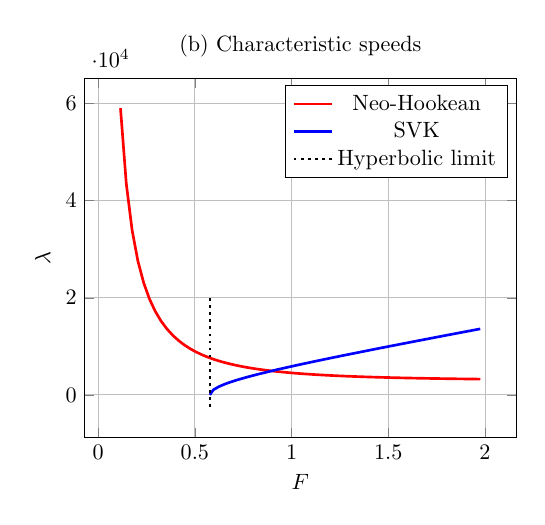
\begin{tikzpicture}[scale=0.8]
\begin{axis}[xlabel=$F$,ylabel=$\abs{\lambda}$,ymajorgrids=true,xmajorgrids=true,title={(b) Characteristic speeds}]
\addplot[Red,very thick] coordinates {(0.11547005383792518,59012.035730808406) (0.14547005383792516,43444.15680640866) (0.17547005383792513,33909.66271892359) (0.20547005383792513,27551.616086072518) (0.23547005383792513,23052.45426344622) (0.2654700538379251,19726.297080765253) (0.2954700538379251,17183.410876622853) (0.3254700538379251,15187.108927674422) (0.35547005383792507,13585.92851121213) (0.38547005383792504,12278.756336822797) (0.415470053837925,11195.691489974464) (0.44547005383792504,10286.970773511453) (0.475470053837925,9516.269220270638) (0.505470053837925,8856.492138358943) (0.535470053837925,8287.045413546242) (0.5654700538379249,7792.014425579814) (0.595470053837925,7358.918900548452) (0.625470053837925,6977.8428382999955) (0.6554700538379249,6640.81463208358) (0.6854700538379249,6341.3576871839605) (0.7154700538379248,6074.159484360366) (0.7454700538379249,5834.824367261866) (0.7754700538379249,5619.6864514897625) (0.8054700538379248,5425.666332338412) (0.8354700538379248,5250.16012367266) (0.8654700538379249,5090.952654625974) (0.8954700538379248,4946.148920983796) (0.9254700538379248,4814.119475233549) (0.9554700538379248,4693.456563660641) (0.9854700538379247,4582.938625301644) (1.0154700538379247,4481.501352586511) (1.0454700538379247,4388.21394243672) (1.0754700538379247,4302.259484218307) (1.1054700538379247,4222.918668359039) (1.1354700538379248,4149.556178447647) (1.1654700538379246,4081.609265724866) (1.1954700538379246,4018.57810915085) (1.2254700538379246,3960.0176447237714) (1.2554700538379246,3905.530610294456) (1.2854700538379247,3854.761601089376) (1.3154700538379245,3807.391969723345) (1.3454700538379245,3763.135435049281) (1.3754700538379245,3721.7342885593334) (1.4054700538379246,3682.9561065868374) (1.4354700538379246,3646.590892305437) (1.4654700538379246,3612.448584281259) (1.4954700538379244,3580.3568787248346) (1.5254700538379244,3550.1593210921387) (1.5554700538379245,3521.7136296737963) (1.5854700538379245,3494.8902195829423) (1.6154700538379245,3469.5709003379666) (1.6454700538379243,3445.6477242208375) (1.6754700538379244,3423.021965921998) (1.7054700538379244,3401.6032167766175) (1.7354700538379244,3381.308579249105) (1.7654700538379244,3362.061949309672) (1.7954700538379245,3343.793376030597) (1.8254700538379243,3326.438489161275) (1.8554700538379243,3309.9379866615427) (1.8854700538379243,3294.237175216221) (1.9154700538379243,3279.2855576483526) (1.9454700538379244,3265.0364619174256) (1.9754700538379242,3251.446707051308) };
\addplot[Blue,very thick] coordinates {(sqrt(1./3.),0.) (0.595470053837925,1048.9455179543422) (0.625470053837925,1731.1029259571128) (0.6554700538379249,2233.012146664284) (0.6854700538379249,2658.790029377158) (0.7154700538379248,3040.5889001561395) (0.7454700538379249,3393.286396027051) (0.7754700538379249,3725.1576526965905) (0.8054700538379248,4041.336632315833) (0.8354700538379248,4345.250197655363) (0.8654700538379249,4639.309436869055) (0.8954700538379248,4925.279696432755) (0.9254700538379248,5204.494537554574) (0.9554700538379248,5477.987035494905) (0.9854700538379247,5746.574266198714) (1.0154700538379247,6010.9138156437175) (1.0454700538379247,6271.542813975518) (1.0754700538379247,6528.905643538706) (1.1054700538379247,6783.374072186155) (1.1354700538379248,7035.262182069363) (1.1654700538379246,7284.837637447764) (1.1954700538379246,7532.330323596269) (1.2254700538379246,7777.939063134427) (1.2554700538379246,8021.836903239133) (1.2854700538379247,8264.175324905573) (1.3154700538379245,8505.087628335128) (1.3454700538379245,8744.691681060722) (1.3754700538379245,8983.092167747032) (1.4054700538379246,9220.382446402957) (1.4354700538379246,9456.646090866763) (1.4654700538379246,9691.958181097758) (1.4954700538379244,9926.386389147965) (1.5254700538379244,10159.991898394823) (1.5554700538379245,10392.830185782268) (1.5854700538379245,10624.951690800193) (1.6154700538379245,10856.402390269113) (1.6454700538379243,11087.224294354115) (1.6754700538379244,11317.455876364773) (1.7054700538379244,11547.132446624275) (1.7354700538379244,11776.286478876727) (1.7654700538379244,12004.947896244235) (1.7954700538379245,12233.144322567889) (1.8254700538379243,12460.901304010209) (1.8554700538379243,12688.242505014787) (1.8854700538379243,12915.189882077482) (1.9154700538379243,13141.763838254037) (1.9454700538379244,13367.983360890252) (1.9754700538379242,13593.866144695845) };
\addplot[dotted,very thick] coordinates {(sqrt(1./3.),-0.25e4) (sqrt(1./3.),2.e4)};
\legend{Neo-Hookean,SVK,Hyperbolic limit}
\end{axis}
\end{tikzpicture}
 \phantomsubcaption \label{subfig:SVK_NH_speeds}}
    \caption{Comparison of neo-Hookean and Saint-Venant-Kirchhoff hyperelastic models.}
    \label{fig:SVK-NH}
  \end{figure}
  At last, figure \ref{fig:SVK-NH}\subref{subfig:SVK_NH_Pi} shows the non-physical behavior of Saint-Venant-Kirchhoff model for high-compression loads that lead to a stress tensor tending to zero.
\end{remark}


%%% Local Variables:
%%% mode: latex
%%% ispell-local-dictionary: "american"
%%% TeX-master: "../mainManuscript"
%%% End:
\section{Approximate--State Riemann solvers}
\label{sec:riemann_solvers}
It has been seen in the previous section that the complete solution of a Riemann problems in solid dynamics is possible for simple problems. However, such a solution may become complicated for multi-dimensional problems or for other non-linear problems. 
Numerical methods such as Finite Volume Methods \cite{Leveque} require the solution of many Riemann problems within a discretized medium. When dealing with non-linear problems, the exact solution of those problems may increase drastically the computational cost, making the numerical scheme prohibitive. Moreover, numerical procedures often require only little information about the solution of Riemann problems and do not need the complete resolution. In that context, alternative procedures have been developed in order to take into account the characteristic structure of a hyperbolic system by computing an approximate solution of Riemann problems. Approximate Riemann solvers developed for Computational Fluid Dynamics allow to extract information for either flux functions (\textit{HLL, HLLC, Roe} and \textit{Osher} approximate Riemann solvers \cite{Trangenstein}, \cite{Toro}) or for vectors of conserved quantities (\textit{approximate--state Riemann solver} \cite[Ch.9]{Toro}, \cite[Ch.22]{Leveque}). Some of those have been applied to specific problems in solid mechanics problems such as the Osher approximate solver (see \cite{LEE_FVM} and \cite{Haider_FVM}) or the HLLC approximate solver (see \cite{Ortega_HLLD}) for hyperelasticity . We recall here the formulation of the approximate-state Riemann solver for solid mechanics. The approach is then applied to the non-linear problem of section \ref{subsec:charac_nonlinear_problems}.

\subsection{General ideas}
As in the previous section, we consider the Riemann problem in the space direction $\vect{N}$:
\begin{equation}
  \label{eq:RP_approx}
  \begin{aligned}
  &\Qcb_t + \Jbsf\(\Qcb\) \drond{\Qcb}{X_N} = \vect{0}, \\
  &\left\lbrace 
    \begin{aligned}
      & \Qcb(X_N,t=0) = \Qcb^L \quad \text{if } X_N< 0\\
      & \Qcb(X_N,t=0) = \Qcb^R \quad \text{if } X_N> 0
    \end{aligned}
    \right.
  \end{aligned}
\end{equation}
The approach for developing an approximate-state Riemann solver consists in linearizing the problem \eqref{eq:RP_approx} by approximating $\Jbsf$ in the vicinity of $\Qcb^L$ and $\Qcb^R$ by a constant matrix $\bar{\Jbsf}=\Jbsf\(\Qcb^L,\Qcb^R\)$ \cite[Ch.15]{Leveque}. Note that this approximation is valid for small jumps in initial data (\textit{i.e }$\Qcb^L\approx\Qcb^R$) and that $\bar{\Jbsf}$ must ensure hyperbolicity of the system, namely $\bar{\Jbsf}$ has real eigenvalues and a complete set of independent eigenvectors. The approximate matrix also satisfies the consistency condition:
\begin{equation}
  \label{eq:approx_constistency}
  \bar{\Jbsf}\(\Qcb,\Qcb\)=\Jbsf\(\Qcb\)
\end{equation}

Such a matrix can be defined by using the definition of right eigenvectors and characteristic speeds $\Jbsf \Rbsf = \Rbsf \Cbsf \Rightarrow \Jbsf = \Rbsf \Cbsf \Rbsf^{-1}$ in which left-going (\textit{resp. right-going}) characteristics and associated eigenvectors are assumed to depend on $\Qcb^L$ (\textit{resp. on} $\Qcb^R$) only. Namely, one writes:
\begin{align*}
  &\Rbsf = \matrice{\Rcb^1(\Qcb^L),\cdots,\Rcb^I(\Qcb^L),\Rcb^{I+1}(\Qcb^R),\cdots,\Rcb^m(\Qcb^R)} \\
  &\Cbsf=\matrice{c_1(\Qcb^L) & & & & & \\ & \cdots & & && \\ & &c_I(\Qcb^L) & & &\\ & & &c_{I+1}(\Qcb^R)& & \\ & & & &\cdots &\\ &&&&&c_m(\Qcb^R)} 
\end{align*}
where $c_I(\Qcb)$ and $m$ are the highest negative eigenvalue and the dimension of the Jacobian matrix. 

At last, the linearized Riemann problem thus written enables the determination of every state vectors $\Qcb(x,t)$ by following the procedure described in section \ref{subsec:charac_Linear_problems} for linear problems, recalled here for convenience for a system of dimension $m$:
\begin{equation}
  \label{eq:approx_RS}
  \begin{aligned}
    &  \Qcb^R-\Qcb^L=\sum_{i=1}^{m} \Rcb^i\delta^i \\
    &  \Qcb(x,t) =\Qcb^R -\sum_{i=I+1}^{m} \Rcb^i\delta^i \\
    &  \Qcb(x,t) =\Qcb^L+ \sum_{i=1}^{I} \Rcb^i\delta^i
  \end{aligned}
\end{equation}
where the point ($x,t$) lies in the region bounded by the $I$th and $I+1$th characteristics.

\begin{remark}
  Note that since one can define a complete set of independent eigenvectors of the Jacobian matrix, the matrix $\Rbsf$ is non-singular so that $\bar{\Jbsf}$ can be uniquely determined. Moreover, the linearization proposed amounts to considering a heterogeneous medium where $\Qcb^{L}$ and $\Qcb^R$ act as material parameters.
\end{remark}

\subsection{Application: Hyperelastic plane wave}
We finish this section with an illustration of the approximate Riemann solver by considering the plane wave problem in a Saint-Venant-Kirchhoff of section \ref{subsec:charac_nonlinear_problems}.
Recall that the eigenvalues and right eigenvectors matrices read for that problem:
\begin{equation}
  \label{eq:SVK_matrices}
  \Cbsf = \matrice{-c & 0 \\ 0 & c} \quad ; \quad \Rbsf = \matrice{c & -c\\ 1&1} \:,\quad c=\sqrt{\frac{\lambda + 2\mu}{2\rho_0}(3F^2-1)}
\end{equation}
Hence, the linearized problem is written with:
\begin{equation}
  \label{eq:SVK_matrices_linear}
  \Cbsf = \matrice{-c_L & 0 \\ 0 & c_R} \quad ; \quad \Rbsf = \matrice{c_L & -c_R\\ 1&1}
\end{equation}
In section \ref{subsec:charac_Linear_problems}, the expression of the wave strengths vector $\vect{\delta}$ has been established for general linear systems of dimension $2$ (see equation \eqref{eq:wave_strengths}):
\begin{equation}
  \vect{\delta}=\frac{1}{c_R+c_L}\matrice{c_R \Delta F +\Delta v\\ c_L \Delta F -\Delta v}
\end{equation}
leading to the solution $\Qcb $ between the two discontinuous waves:
\begin{equation}
  \label{eq:SVK_approx_solution}
  \Qcb  = \Qcb^L + \delta^1 \Rcb^1 = \matrice{v_L \\F_L} +\delta^1 \matrice{c_L \\1} \quad \text{or} \quad \Qcb  = \Qcb^R - \delta^2 \Rcb^2 = \matrice{v_R \\F_R} -\delta^2 \matrice{-c_R \\1}
\end{equation}
Substitutions of $\delta^{1,2}$ from second equations in first ones provide straight lines equations in the phase plane ($F,v$):
\begin{equation}
  \label{eq:approx_straight}
  v  = v_L + c_L(F -F_L) \quad ; \quad v  = v_R + c_R(F_R-F )
\end{equation}
\begin{figure}[h!]
  \centering
  {\definecolor{Purple}{RGB}{120,28,129}
\definecolor{Blue}{RGB}{63,96,174}
\definecolor{Duck}{RGB}{83,158,182}
\definecolor{Green}{RGB}{109,179,136}
\definecolor{Yellow}{RGB}{202,184,67}
\definecolor{Orange}{RGB}{231,133,50}
\definecolor{Red}{RGB}{217,33,32}
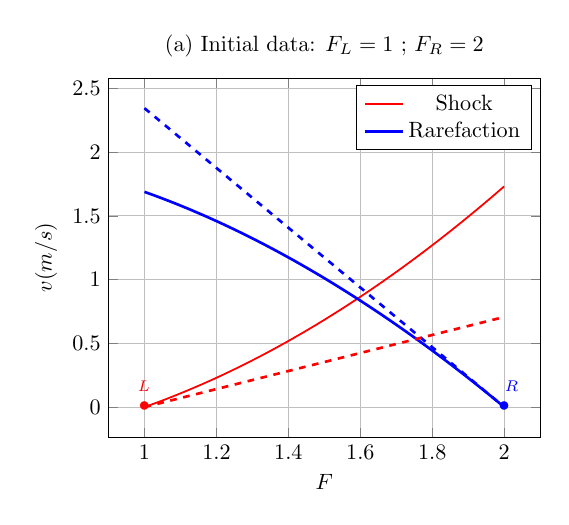
\begin{tikzpicture}[scale=0.8]
\begin{axis}[xlabel=$F$,ylabel=$v (m/s)$,ymajorgrids=true,xmajorgrids=true, title={(a) Initial data: $F_L=1$ ; $F_R=2$}]
  \addplot[Red,thick] coordinates {(1.0,0.0) (1.0196019601960196,0.019889905868838792) (1.0392039203920391,0.04035480171519238) (1.058805880588059,0.06139339246981025) (1.0784078407840785,0.08300445472552491) (1.098009800980098,0.1051868317293367) (1.1176117611761176,0.1279394287977403) (1.1372137213721372,0.1512612091133456) (1.1568156815681567,0.17515118986560513) (1.1764176417641765,0.19960843870261852) (1.196019601960196,0.2246320704646163) (1.2156215621562156,0.25022124417291264) (1.2352235223522352,0.2763751602509047) (1.2548254825482548,0.30309305795616337) (1.2744274427442743,0.330374213004825) (1.2940294029402941,0.3582179353714115) (1.3136313631363137,0.386623567248899) (1.3332333233323332,0.4155904811553686) (1.3528352835283528,0.445118078174895) (1.3724372437243724,0.47520578632153143) (1.3920392039203922,0.5058530590163028) (1.4116411641164117,0.5370593736680643) (1.4312431243124313,0.568824230349938) (1.4508450845084508,0.6011471505637854) (1.4704470447044704,0.6340276760858663) (1.4900490049004902,0.667465367887438) (1.5096509650965095,0.7014598051246006) (1.5292529252925293,0.7360105841921958) (1.5488548854885489,0.7711173178369951) (1.5684568456845684,0.8067796343258441) (1.5880588058805882,0.8429971766647708) (1.6076607660766076,0.8797696018654025) (1.6272627262726274,0.917096580255355) (1.646864686468647,0.9549777948294852) (1.6664666466646665,0.9934129406392047) (1.686068606860686,1.032401724217221) (1.7056705670567056,1.0719438630353144) (1.7252725272527254,1.1120390849929296) (1.7448744874487447,1.1526871279345328) (1.7644764476447645,1.1938877391938512) (1.784078407840784,1.2356406751632294) (1.8036803680368036,1.2779457008865038) (1.8232823282328234,1.320802589673878) (1.8428842884288428,1.3642111227374165) (1.8624862486248626,1.4081710888458763) (1.8820882088208821,1.4526822839976499) (1.9016901690169017,1.4977445111107466) (1.9212921292129215,1.543357579728744) (1.9408940894089408,1.5895213057417645) (1.9604960496049606,1.6362355111215798) (1.9800980098009802,1.6835000236699957) (1.9996999699969997,1.7313146767797576) };
  \addplot[Blue,very thick] coordinates {(1.0,1.6884673989302577) (1.0196019601960196,1.6685781823289632) (1.0392039203920391,1.648117983645035) (1.058805880588059,1.6270917763366024) (1.0784078407840785,1.6055041425368688) (1.098009800980098,1.5833593157699348) (1.1176117611761176,1.5606612177002648) (1.1372137213721372,1.5374134899261505) (1.1568156815681567,1.5136195216278194) (1.1764176417641765,1.48928247372591) (1.196019601960196,1.4644053000848238) (1.2156215621562156,1.4389907661996928) (1.2352235223522352,1.4130414657294894) (1.2548254825482548,1.3865598351776642) (1.2744274427442743,1.3595481669723095) (1.2940294029402941,1.3320086211576845) (1.3136313631363137,1.3039432358761032) (1.3332333233323332,1.2753539367920979) (1.3528352835283528,1.246242545588463) (1.3724372437243724,1.216610787645106) (1.3920392039203922,1.1864602989961286) (1.4116411641164117,1.1557926326474621) (1.4312431243124313,1.12460926432638) (1.4508450845084508,1.092911597724879) (1.4704470447044704,1.0607009692909792) (1.4900490049004902,1.0279786526152188) (1.5096509650965095,0.994745862453826) (1.5292529252925293,0.9610037584250569) (1.5488548854885489,0.9267534484108921) (1.5684568456845684,0.8919959916925568) (1.5880588058805882,0.8567324018451127) (1.6076607660766076,0.8209636494135533) (1.6272627262726274,0.7846906643903794) (1.646864686468647,0.7479143385125069) (1.6664666466646665,0.7106355273934435) (1.686068606860686,0.6728550525050632) (1.7056705670567056,0.6345737030218022) (1.7252725272527254,0.595792237538853) (1.7448744874487447,0.5565113856747698) (1.7644764476447645,0.5167318495678894) (1.784078407840784,0.47645430527509447) (1.8036803680368036,0.43567940408061234) (1.8232823282328234,0.3944077737218566) (1.8428842884288428,0.3526400195386741) (1.8624862486248626,0.31037672555176576) (1.8820882088208821,0.2676184554755838) (1.9016901690169017,0.22436575367049583) (1.9212921292129215,0.18061914603862234) (1.9408940894089408,0.13637914086738703) (1.9604960496049606,0.09164622962443836) (1.9800980098009802,0.04642088770736517) (1.9996999699969997,0.0007035751512764867) };
  \node at (axis cs:1,0) [Red] {$\bullet$};
  \node at (axis cs:2.,0) [Blue] {$\bullet$};
  \node at (axis cs:1,0) [anchor=south,Red] {$\Qcb^L$};
  \node at (axis cs:1.98,0) [above right,Blue] {$\Qcb^R$};
  \addplot[Blue,dashed,very thick,domain=1:2,samples=51,samples y=0]
    ({x},{0.-sqrt(0.5*(12.-1))*(x-2.)});
  \addplot[Red,dashed,very thick,domain=1:2,samples=51,samples y=0]
    ({x},{0.+sqrt(0.5*(2.-1))*(x-1.)});
  \legend{Shock,Rarefaction}
\end{axis}
\end{tikzpicture}
 \phantomsubcaption \label{subfig:SVK_Approx1}}
  {\definecolor{Red}{RGB}{217,33,32}
\definecolor{Blue}{RGB}{63,96,174}
\definecolor{Duck}{RGB}{83,158,182}
\definecolor{Green}{RGB}{109,179,136}
\definecolor{Yellow}{RGB}{202,184,67}
\definecolor{Orange}{RGB}{231,133,50}
\definecolor{Purple}{RGB}{120,28,129}
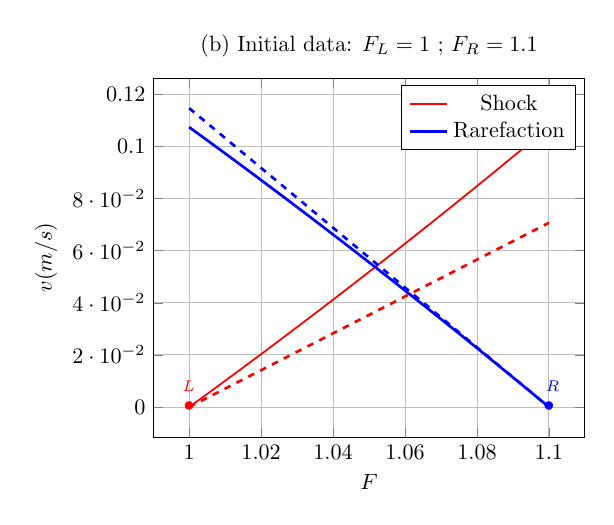
\begin{tikzpicture}[scale=0.8]
\begin{axis}[xlabel=$F$,ylabel=$v (m/s)$,ymajorgrids=true,xmajorgrids=true,title={(b) Initial data: $F_L=1$ ; $F_R=1.1$}]
\addplot[Red,thick] coordinates {(1.0,0.0) (1.001960196019602,0.0019630775609053948) (1.003920392039204,0.003931917267080632) (1.005880588058806,0.005906517718693416) (1.0078407840784078,0.007886877524091035) (1.00980098009801,0.009872995299740863) (1.0117611761176117,0.011864869670167599) (1.0137213721372138,0.01386249926789511) (1.0156815681568157,0.01586588273338493) (1.0176417641764177,0.01787501871497885) (1.0196019601960196,0.019889905868838792) (1.0215621562156216,0.02191054285889049) (1.0235223522352235,0.023936928356764118) (1.0254825482548255,0.025969061041739377) (1.0274427442744274,0.028006939600686957) (1.0294029402940295,0.030050562728014697) (1.0313631363136313,0.03209992912561001) (1.0333233323332334,0.034155037502787186) (1.0352835283528352,0.0362158865762309) (1.0372437243724373,0.03828247506994398) (1.0392039203920391,0.04035480171519238) (1.0411641164116412,0.04243286525045405) (1.0431243124312433,0.044516664421364406) (1.045084508450845,0.04660619798066565) (1.0470447044704472,0.048701464688155255) (1.049004900490049,0.050802463310633685) (1.050965096509651,0.05290919262185532) (1.052925292529253,0.055021651402476585) (1.054885488548855,0.05713983844000798) (1.0568456845684568,0.059263752528762766) (1.058805880588059,0.06139339246981025) (1.0607660766076608,0.06352875707092508) (1.0627262726272628,0.06566984514654145) (1.0646864686468647,0.06781665551770343) (1.0666466646664667,0.06996918701201955) (1.0686068606860686,0.07212743846361445) (1.0705670567056706,0.07429140871308419) (1.0725272527252725,0.07646109660744838) (1.0744874487448746,0.07863650100010654) (1.0764476447644764,0.08081762075079126) (1.0784078407840785,0.08300445472552491) (1.0803680368036805,0.08519700179657394) (1.0823282328232824,0.08739526084240548) (1.0842884288428845,0.08959923074764438) (1.0862486248624863,0.09180891040302837) (1.0882088208820884,0.09402429870536706) (1.0901690169016902,0.09624539455749745) (1.0921292129212923,0.09847219686824406) (1.0940894089408941,0.1007047045523746) (1.0960496049604962,0.10294291653056116) (1.098009800980098,0.1051868317293367) (1.0999699969997,0.10743644908105657) };
\addplot[Blue,very thick] coordinates {(1.0,0.1073874627707086) (1.001960196019602,0.10542438591418365) (1.003920392039204,0.10345555112494406) (1.005880588058806,0.10148096397787983) (1.0078407840784078,0.09950062999930058) (1.00980098009801,0.09751455466754301) (1.0117611761176117,0.09552274341357074) (1.0137213721372138,0.09352520162156171) (1.0156815681568157,0.0915219346294884) (1.0176417641764177,0.089512947729686) (1.0196019601960196,0.08749824616941433) (1.0215621562156216,0.08547783515140679) (1.0235223522352235,0.08345171983441528) (1.0254825482548255,0.08141990533374051) (1.0274427442744274,0.07938239672176006) (1.0294029402940295,0.07733919902844166) (1.0313631363136313,0.0752903172418546) (1.0333233323332334,0.07323575630866758) (1.0352835283528352,0.07117552113464229) (1.0372437243724373,0.06910961658511733) (1.0392039203920391,0.06703804748548585) (1.0411641164116412,0.06496081862166392) (1.0431243124312433,0.06287793474055453) (1.045084508450845,0.06078940055050131) (1.0470447044704472,0.05869522072173673) (1.049004900490049,0.056595399886824015) (1.050965096509651,0.05448994264109064) (1.052925292529253,0.05237885354305752) (1.054885488548855,0.05026213711485809) (1.0568456845684568,0.0481397978426566) (1.058805880588059,0.04601184017705303) (1.0607660766076608,0.04387826853348905) (1.0627262726272628,0.0417390872926421) (1.0646864686468647,0.0395943008008181) (1.0666466646664667,0.037443913370333926) (1.0686068606860686,0.03528792927989956) (1.0705670567056706,0.03312635277498877) (1.0725272527252725,0.03095918806820985) (1.0744874487448746,0.02878643933966615) (1.0764476447644764,0.026608110737315303) (1.0784078407840785,0.0244242063773199) (1.0803680368036805,0.022234730344396287) (1.0823282328232824,0.020039686692156212) (1.0842884288428845,0.017839079443443134) (1.0862486248624863,0.01563291259066641) (1.0882088208820884,0.013421190096127349) (1.0901690169016902,0.011203915892344065) (1.0921292129212923,0.008981093882367926) (1.0940894089408941,0.006752727940100287) (1.0960496049604962,0.00451882191059879) (1.098009800980098,0.0022793796103861676) (1.0999699969997,3.4404827748516585e-05) };
\node at (axis cs:1,0) [Red] {$\bullet$};
  \node at (axis cs:1.1,0) [Blue] {$\bullet$};
  \node at (axis cs:1,0) [anchor=south,Red] {$\Qcb^L$};
  \node at (axis cs:1.097,0) [above right,Blue] {$\Qcb^R$};
  \addplot[Red,dashed,very thick,domain=1:1.1,samples=51,samples y=0]
  ({x},{0.+sqrt(0.5*(2.-1))*(x-1.)});
  \addplot[Blue,dashed,very thick,domain=1:1.1,samples=51,samples y=0]
    ({x},{0.-sqrt(0.5*(3.*(1.1^2)-1))*(x-1.1)});
\legend{Shock,Rarefaction}
\end{axis}
\end{tikzpicture}
 \phantomsubcaption \label{subfig:SVK_Approx4}}
  \caption{Comparison of approximate (dashed lines) and exact (solid lines) solution for a one-dimensional strain problem in a Saint-Venant-Kirchhoff hyperelastic material}
  \label{fig:comparison_exact_approx}
\end{figure}
The intersection of those straight lines in the phase plane corresponds to the approximate solution. Figure \ref{fig:comparison_exact_approx} shows comparisons of approximate and exact solutions for various initial data, all leading to a $1$-shock--$2$-rarefaction exact solution. As expected, approximate and exact solutions are different and get closer for small initial discontinuities, falling in the linearization assumption $\Qcb^L\approx \Qcb^R$. As a consequence, in figures \ref{fig:comparison_exact_approx}\subref{subfig:SVK_Approx1} a big initial discontinuity is considered so that the approximation error is larger than that of figure \ref{fig:comparison_exact_approx}\subref{subfig:SVK_Approx4} for which initial data are based on a weak jump.


%%% Local Variables:
%%% mode: latex
%%% TeX-master: "../mainManuscript"
%%% End:


\section{Conclusion}
It has been seen in this chapter that solid dynamics balance equations can be written as a first order hyperbolic system whose theory has been recalled in section \ref{sec:PDEs}.
Indeed, the thermodynamics framework assuming generalized standard materials combined with conservation laws allowed in section \ref{sec:solidMech_equations} the building of conservative or quasi-linear forms.
Those systems of partial differential equations admit non-complex eigenvalues and independent eigenvectors provided that some requirements on the stored energy function are satisfied (positive definiteness of the acoustic tensor).
Then, the characteristic analysis of the quasi-linear form in section \ref{sec:characteristic_analysis} enabled the highlighting of specific wave types involved in the solutions of dynamic problems, that is: discontinuous, shock and simple waves.
Even though exact solutions of linear and non-linear problems have been developed in section \ref{sec:riemann_problems}, it is not possible in general, hence the introduction of approximate-state Riemann solvers in section \ref{sec:riemann_solvers}.
This solution strategy will be used in what follows as an element of the \textit{Discontinuous Galerkin Material Point Method}, which is the object of the next chapter.

%%% Local Variables:
%%% mode: latex
%%% TeX-master: "../mainManuscript"
%%% End:
